%% \documentclass[sigconf,10pt]{acmart}
%% \documentclass[sigalternate,10pt]{acmart}
\documentclass{sig-alternate-10pt}
\pdfpageheight=11in
\pdfpagewidth=8.5in

% Added packages
\usepackage{soul,xcolor}
\usepackage{enumitem,color}
\setlist{leftmargin=5.5mm}
\usepackage{array}
\usepackage{booktabs} % For formal tables
\usepackage{xspace}
\usepackage{multirow}
\usepackage{makecell}
\usepackage{graphicx,amssymb,amsmath,endnotes}
\usepackage{ulem}
\usepackage{subcaption}
\usepackage{wrapfig}
\usepackage{fancyhdr}
\fancyhead{}
\fancyfoot{}
\fancyfoot[C]{\thepage}
%\usepackage{textcomp, libertine}
\usepackage{hyperref}
\usepackage{url}
\def\UrlBreaks{\do\/\do-}
\renewcommand{\UrlFont}{\ttfamily\small}
% Copyright
% \setcopyright{none}
% \renewcommand\footnotetextcopyrightpermission[1]{}	% Remove this in camera ready
% \settopmatter{printfolios=true} 
% \settopmatter{printacmref=false}
\pagestyle{plain}
\normalem

\title{Experience: Feasibility of Self Constructive Component-Wise Power Modeling on Modern Smartphones}
\author{
Paper ID:77  pages = 12+2
% Anonymous Author(s)
}


\newcommand{\oldstuff}[1]{}
\newcommand{\yes}{$\checkmark$}
\newcommand{\limited}{Limited}
\newcommand{\no}{$\times$}
% \definecolor{gray}{rgb}{0.5,0.5,0.5}
\newcommand{\etc}{{\it etc.}\xspace}
\newcommand{\etcc}{{\it etc.}}
\newcommand{\ie}{{\it i.e.,}\xspace}
\newcommand{\eg}{{\it e.g.,}\xspace}
\newcommand{\etal}{\emph{et al.}\xspace}
\newcommand{\SmallCrunch}{\vspace{-0cm}}
\newcommand{\smallcrunch}{\vspace{-0cm}}
\newcommand{\questionaj}[1]{{\it #1}}
\newcommand{\updated}[1]{{\it {}}}
%\newcommand{\updated}[1]{{\color{red} {updated: #1}}}
\newcommand{\editaj}[2]{{\sout{#1}\color{red} {#2}}}
\newcommand{\removeaj}[2]{{\color{red}{\textbf{Remove following:}}}{\sout{#1}}	{\color{red} {\textbf{Because} #2}}}
\newcommand{\addaj}[1]{{\color{red} {ADD?: #1}}}
%\newcommand{\highlight}[1]{{\color{blue}#1}}
\newcommand{\insitu}{{\em in situ}\xspace}
\newcommand{\name}{{\sc PFOP}\xspace}
\newcommand{\namee}{{\sc PFOP}}
\newcommand{\ychurm}[1]{{\hspace{-0.2cm}}}
\newcommand{\panic}[1]{\vspace{-#1 plus 1pt minus 1pt}}
\newcommand{\panictwo}[1]{\vspace{-#1 plus 2pt minus 2pt}}
% \newcommand{\nsection}[1]{\panictwo{0pt}\section{#1}\panictwo{0pt}}
% \newcommand{\nsubsection}[1]{\panictwo{0pt}\subsection{#1}\panictwo{0pt}}
% \newcommand{\nsubsubsection}[1]{\panictwo{0pt}\subsubsection{#1}\panictwo{0pt}}
\newcommand{\flow}{flow\xspace}

\newcommand{\aj}[1]{{\color{blue} {\em #1}}}
\renewcommand{\st}[1]{}
% \newcommand{\comment}[1]{{\color{red} \it #1}}
\newcommand{\comment}[1]{{\em \it #1}}
% \newcommand{\comment}[1]{}

\newcommand{\forjnl}[1]{{}}
\newcommand{\dcomment}[1]{{\color{blue} #1}}
\newcommand{\expr}[1]{{\color{red} Experiments: #1}}
\newcommand{\coflowone}{C_1}
\newcommand{\coflowtwo}{C_2}
\newcommand{\nexuserror}{19.4\%\xspace}
\newcommand{\pixelerror}{23.8\%\xspace}
\newcommand{\motoerror}{13.4\%\xspace}
\newcommand{\nexuserrorreduction}{5.9$\times$\xspace}
\newcommand{\pixelerrorreduction}{7.2$\times$\xspace}
\newcommand{\motoerrorreduction}{4.6$\times$\xspace}
\newcommand{\revv}[1]{{#1}}
\newcommand{\tabincell}[2]{\begin{tabular}{@{}#1@{}}#2\end{tabular}}
\newcolumntype{P}[1]{>{\centering\arraybackslash}p{#1}}
\renewcommand{\paragraph}[1]{{\vspace{0.1in} \noindent \bf #1}}

\newcommand*\rot{\rotatebox{90}}

\newcommand{\cut}[1]{{}}

\date{May 2020}

\begin{document}
\setstcolor{red}

\maketitle
\begin{abstract}

Power modeling of mobile device components is foundational to mobile app energy
	drain analysis such as for energy profiling and energy debugging, and to
	mobile OS design such as %runtime power management 
	for battery-drain accounting and energy-aware
	scheduling.  Traditional power model derivation (TPMD) is an offline process
	based on microbenchmarks
% to drive each mobile device component into each possible power state to
	% record its power draw (from a power monitor) 
	but it is a time consuming process, taking several weeks of manual effort
	to derive a phone's power model, and is often not comprehensive-- it misses
	the dependence of component power behavior on model parameters not considered
	at the modeling time such as battery age and differing mobile network
	behavior in different geographies. Thus, porting mobile OSes, such as
	Android, over to new devices adds an additional overhead for OEMs to provide
	a power model.  \comment{I've seen these to be just copy-pasted from
	other devices and to be wrong in many cases, can we make such a claim, do we
	have some examples? Yes.
	Android power profile is stored in power\_profile.xml~\cite{androidpowerprofile}.
	We found out that Pixel 4 and Pixel 2 share the same settings
	whereas the CPU are from different generations of SoC.}
	Similarly, due to the tedious nature of
	TPMD, energy profilers have not been able to become plug-and-play.
	Commercial mobile energy profilers either support a handful of devices or show
	very coarse results. Further, since power models generated from TPMD are not comprehensive, mobile
	energy profilers can show inaccurate results that can confuse developers.

	% app usage, the mobile device, and environment such as the battery age.}
% or device temperature. 
In contrast, self-constructive power model derivation (SPMD)
	promises to overcome these shortcomings of TPMD by collecting 
% each actual power state that each device component ran under, the
	% utilization, and 
component power state and utilization, total device energy drain during an app
	run, and deriving the power model parameters by regression using a system of
	linear equations.  
%	\st{Though first proposed almost a decade ago, SPMD has
%	only been explored so far for energy drain estimation with a finer resolution
%	(e.g. 10ms) compared to the device power sensor readings (e.g. 1s). }
	Although first proposed almost a decade ago, SPMD has only been
	explored so far for enhancing the resolution for total energy drain.
	In this paper, we report our experience of applying SPMD in deriving
	{\it component-wise} power models for modeling 
	%component-wise 
	energy consumption on 3 modern
	smartphones. 
	% Accurate component-wise power models are necessary for the 
	% design of energy profilers and energy-aware schedulers. In this paper, we explore
	% the feasibility of SPMD on modern smartphones. We find that the time window granularity 
	% used for setting up the systems of equations plays a major roles in the success of SPMD
	% and show promising results of applying SPMD to quickly generate comprehensive component
	% power models for three modern devices.
	%, which potentially provide more valuable information for
	%real-world application (e.g., diagnosing power draw , battery scheduling)
	%than just enhancing resolution of energy drain estimation. 
	%By our experiment,
	Overall, we find that the measurement noise and lack of equation diversity 
	greatly impact the modeling results of
	SPMD, especially when sampling frequency is low. When using higher sampling
	frequency, we get relatively better modeling results, but is still not good
	enough to be used in practice.
	% , which suggests that the utilization of SPMD on
	% modern smartphones has a high requirement on the quality of measuring and
	% sampling.
	

\st{
In this paper, we experimentally study 
the feasibility of SPMD in deriving component-wise power models 
for modern smartphones. Our study shows that SPMD faces a 
fundamental dilemma: it can only be used for the particular 
app scenario as even different scenarios of the same app result 
in different power models; on the other hand, when 
restricted to a particular app scenario, the system of 
equations lacks diversity when created at the per-second granularity, 
preventing the regression solver from generating meaningful model parameters.  
%  Finally, we show
% zooming into the millisecond scale in setting up equations can overcome the diversity problem 
% but the equation can be dominated by measurement noise, and further SPMD would not scale
% as a 1-minute app run would require solving thousands of systems of equations. 
Our study suggests that it is extremely challenging to derive component-wise power model parameters for modern smartphones using SPMD. }


\if 0
In this paper, we perform an in-depth investigation of the feasibility of SPMD in deriving accurate per-component power models for modern smartphones. 
 % We systematically explore the time-scale for setting up the system of equations, ranging from macro-scale (one equation per second), to micro-scale (two equations per rendering interval to exploit GPU Busy and Idle power states), to nano-scale (16 equations per rendering interval to explore diversity within each rendering interval.)
We find that while conceptually simple, in practice it is 
extreme difficult to create a system of equations that 
exhibit sufficient diversity which poses two challenges 
to the regression solver to generate meaningful per-component 
power model parameters: (1) lack of diversity in phone
component usage which leads to the rank of the equations 
(right-hand-side of equations) to be smaller than the number 
of unknowns (model parameters); (2) noise in energy drain 
readings (left-hand-side of the equations) which results 
in contradicting component usage and energy drain. Our 
experimental results suggest that while SPMD may be useful for
energy modeling which only requires a good fitting of the two 
sides of the equations, it remain not practical for deriving 
per-component power model parameters for use in mobile app 
energy drain analysis such as energy profiling and energy debugging. 

%   We believe that our  ndings can encourage further research and standardization e orts towards higher utilization of commercialized CIoT network infrastructures.
\fi

\end{abstract}

\pagestyle{plain}

\section{Introduction}
\label{sec:motivation}

\subsection{Background and Motivation}
\label{subsec:back}


% In this section, we provide a brief background and motivation for self-power modeling of mobile devices, and discuss the prior-art. 

% \subsection{Power Modeling of Mobile Devices}

Modern smartphones come with a wide variety of hardware components
, \eg CPU, GPU, WiFi and LTE NIC, and OLED display. To offer rich 
user experience, mobile apps running on the phone often utilize 
several of these components simultaneously, each of these 
drawing power contributing  to the overall total phone power draw.

Diagnosing and managing the power draw of smartphones using \aj{just} an external power monitor or the phone 
built-in power sensor  (available in most smartphones today)
are difficult as they can only measure the total phone power draw.
Power modeling is a technique that allows breaking down the 
total phone power draw into the power draw by individual components, 
and is the foundation for various mobile device power
management solutions such
as mobile software energy profiling~\cite{flinn:1999,shye2009into,zhang2010accurate,sesame:2011,pathak2012energy,appscope,ding2017gfxdoctor,facebookbatterymetrics}, energy debugging~\cite{ma2013edoctor,benerjee:2014}, and in-the-wild energy measurement~\cite{chen:sigm2015,androidbatterystats,androidvitals}.  

% A power model for each phone component captures the mathematical correlation between the {\it events} that {trigger} the usage of the component and the resulting component power draw; it is a function takes power events for a given phone component as input and outputs the estimated power draw for that component due to those events.
{
Each of the phone components can potentially be 
in different power states, drawing different amount of power. 
An empirical power model for a component captures the power 
draw while the component in each of the possible power state, known as  the {\em power model parameter}.
%
Once derived, a component’s power model can be used to estimate 
the energy drain of the component during the runtime of any app. 
This is achieved by collecting the duration (utilization) that 
the component spends in each power state during the app run
and in post-processing summing up the product of 
each utilization duration with its corresponding power draw from the power model.
}

\paragraph{Traditional Power Model Derivation.}
\label{subsec:tpmd}
Traditional power model derivation (TPMD) is an offline, largely manual process. 
\if 0
It runs microbenchmarks on the phone to exercise the phone components 
in isolation to induce the power triggering events. The triggers 
associated with each component are captured along with the 
instantaneous power measured using an external power monitor 
or the built-in power sensor. Next, the power used by each 
phone component is isolated and the power model is derived 
by extracting the correlation between the triggers and the components’ power draw.
\fi
It consists of four major steps: 
%
(1) Enumerate all the power states that each component can possibly enter;  
% 
(2) develop  microbenchmarks that drive the component into each of these 
possible power states; 
%
(3) run the microbenchmark while collecting the component power draw online; and 
%
(4) in offline processing, 
align the power draw timeline with the microbenchmark execution 
to find the power draw corresponding to each of the power states 
that the component was running in. If a component cannot be exercised alone,
\eg the WiFi NIC cannot be exercised alone without packet 
processing in the CPU, the power model for the component needs 
to be derived incrementally (see \S\ref{sec:primer} for an example.)

Although conceptually simple, traditional power model derivation suffers several major drawbacks
in practice. 

\aj{
{\it Labor-intensive manual process.}
Further, TPMD is a laborious process that faces many practical challenges:
(1) Connecting an external power source to a commodity phone is challenging.
The technique requires a soldering station and the skills to disassemble 
the device and solder the power monitor wires to the power management circuit.
% For example Moto Z3 and Nexus6 have different arrangements.
%i.e Nexus6 only the back cover has to be removed and probes are connected whereas Z3 requires the total disassembly and removal of the battery.
%(2) Writing microbenchmarks that force components into different power states require
(2) The entire process is time consuming.
For example, the CPU of the Moto Z3 phone released in August 2018 comes with 4 big 
cores that can be adjusted among 31 frequencies and
4 LITTLE cores that can be adjusted among 22 frequencies.
To derive the CPU model, a benchmark is run at each core at each CPU frequency 
% with 100\% CPU utilization
for a certain duration and the process is repeated for all the big.LITTLE core-frequency combinations.
% Some of these frequency combinations may never appear in a real app run.
% \st{
% {\it (1) App usage dependence.}
% {The most serious drawback of offline power model derivation 
% using microbenchmarks is the modeling error 
% from not able to capture {\it power state variations} for any particular app execution.  
% }
% A power state variation for a component happens when different 
% functional units inside the component are exercised under different 
% app usage. As a result, the amount of power the component draws varies  . 
% An example of this is while the CPU is running in the same frequency with  100\% utilization, 
% integer arithmetic workload and floating point  arithmetic workload can lead to 13.5\% 
% different CPU power draw running at 2.45GHz on Moto Z3.
% The number of possible power state variations can also be unknown or simply 
% too many to enumerate.}

This cumbersome process inhibits quickly developing power models for diverse phones
% Because of the laborious nature of TPMD, 
and due to this, energy profilers have not been able to
become plug-and-play.  AT\&T's Video Optimizer~\cite{aro}, for example, only
supports handful of devices. Android Energy
Profiler~\cite{androidenergyprofiler} resorts to showing energy consumptions as
Low, Medium, and High, instead of showing accurate quantitative energy drain
results.


{\it Hidden or costly model parameters.}
First, TPMD assumes all the exact power states for each component are known and are modeled during offline model derivation. In practice, this is hard do for several reasons:
(1) the microbenchmark author may not be aware of every trigger that can impact component power draw, \eg battery age can impact ??? ;
(2) power triggers may not be accessible during logging such as at the time of a profile run or may not allow modification by microbenchmarks \eg GPU
(should this be CPU??) memory utilization; and
(3) the number of possible power triggers can be too fine-grained and hence too expensive to enumerate \eg int-ops vs flops.
%(3) enumerating all possible power state variations may not be
%necessarily useful as many combinations of power state variations 
%(of different components) may not appear in real apps.
%
% (3) logging all triggers can be prohibitively expensive or not allowed by the OS. 
%  In practice, there are possible hidden triggers not captured in the power models  which may be exercised differently by different apps~\cite{dong2011self}. 

For these reasons, the TPMD-derived power models 
are typically not comprehensive as they do not model all power triggers and hence
do not capture the actual component power draw behavior during a particular app run
which can lead to significant model error. 
}

% \st{
% {\it (2) Device and environment dependence.}
% In addition, power models are phone-specific and hence the TPMD process needs to be repeated,
% \eg by an OEM phone vendor for all its phone models. 
% Furthermore, even two devices of the same model can have different 
% power models depending on the age of the device battery and effect of 
% external factors such as phone temperature.These factors require 
% the power models to be re-derived.}

\paragraph{Self-constructive Power Model Derivation.}
\label{subsec:spmd}
%
Self constructive power model derivation (SPMD)~\cite{dong2011self} 
has the potential to overcome 
% the app usage/device/ environment dependencies 
these limitations of TPMD and can enable easier portability of 
many energy diagnostics solutions such as energy profilers~\cite{flinn:1999,shye2009into,zhang2010accurate,sesame:2011,pathak2012energy,appscope,ding2017gfxdoctor,facebookbatterymetrics} and energy-aware schedulers.
Instead of developing and running microbenchmarks to drive the 
phone component into each of the possible power states
which still cannot capture
all power state variations, SPMD collects details of each of the 
actual power states that each phone component ran under, the 
utilization (duration) in that state, and the total phone power draw 
using the power sensor or power monitor  during each actual 
app run. In post-processing, SPMD sets up and solves a system of equations 
that express the total phone energy drain for each of the time 
interval as the sum of the energy drain for all the components, which 
are linear functions of component power draws, 
\ie each model parameter multiplied by the corresponding utilization.

Thus SPMD is "in-situ"; the component power models are generated 
at the end of each app run, and hence SPMD avoids the time-consuming 
manual model derivation in TPMD.
Second, SPMD is intrinsically phone-specific and app-run-specific, 
and adapts with environment factors that can affect component power 
draw such as the battery age, phone temperature, intops vs flops, and GPU memory utilization.
% Finally, SPMD is intrinsically specific to
% each app run and hence the relevant phone component usage and power 
% draw scenario. 
% As such,
% {it captures only the relevant power states and power state variations
% that contribute to each 
% phone component power draw during specific app run.} 
Such intrinsic handset, environment, and app specificities make SPMD 
likely to generate more accurate power models than TPMD; 
although the derived model may not contain all possible model parameters,
it will contain all the model parameters that are needed to analyze 
the energy drain of that particular app run. 

% \if 0
% The power consumed by a smartphone heavily depends on its hardware components and configurations.
% Due to it's nature, traditional power modeling provides fixed models.
% Different apps uses various hardware components to a varying extent with inter-component interactions, which may not be modelled by a fixed power model.
% 
% As self modeling is done on device, it is inherently environment agnostic and leads to accurate power modeling.
% 
% \fi

\paragraph{Prior Work: Sesame.}
\label{sec:back}
%
Sesame~\cite{dong2011self} was one of the first work to demonstrate 
the feasibility of self power model derivation.\footnote{We distinguish SPMD from self-metering work such as~\cite{zhang2010accurate,devscope:2012} 
which used built-in battery interfaces to measure the power or 
use regression but still used training microbenchmarks to 
exercise one phone component at a time.
% and hence the models derived are not app usage agnostic.  
}
% Few application of modelling as stated in Sesame could be detecting rogue applications and adding support to OS for determining adequate measures in optimizing battery life in a classical way.
% Various  models developed in  classical way are also influenced by the variable internal resistance of the device battery.
% Sesame also mentions that traditional energy models of 1 Hz are fundamentally inadequate for applications such as per-application energy accounting.
% Sesame idea is to devise a model molding method that achieves high accuracy and high rate when combined with principal component analysis and to realize Sesame on resource-limited mobile devices (as it is impractical to include all predictors that can account for every hardware detail because not all hardware components are visible to the OS and collecting the values of a large number of predictors would incur significant overhead).
However, its motivation and design goals were not on constructing
{\it component-wise} power models. Instead, its primary goals were (1)
modeling the whole phone energy drain at a higher rate, \eg 100 Hz,
than what the built-in power sensor could provide, \eg 1Hz, and (2)
doing so without an external high-resolution power monitor so that the model
could be "personalized" for a given app on a given device.
% The primary motivations of Sesame are (1) to improve model accuracy by eliminating the model dependencies on hardware, app usage and battery conditions; and (2) to ease model derivation by automatically generating energy models without external assistance.
%    \item Utilize real usage of every individual user to generate personalized energy models and to adapt % such models for potentially higher accuracy
%
% \if 0
% However, though Sesame~\cite{dong2011self} pioneered the concept 
% of self power modeling, the study which was conducted over a decade 
% ago had two major limitations.
% First, it focused on fine-resolution whole-phone energy drain 
% estimation, \eg the total phone energy drain at fine-resolutions, 
% as opposed to per-phone-component power or energy drain estimation.
% \fi 
In particular, it uses battery State-of-Charge (SoD) readings to 
set up energy drain equations at the power sensor sampling 
resolution (\eg 1s), and uses the solutions to the unknowns to 
directly estimate the total energy drain at finer time-scales, \eg 10ms.
The work did not study the accuracy of component power parameters derived.

% However it is important to note that Sesame can incorporate any predictor that can be acquired in software. Sesame further utilizes the Advanced Configuration and Power Interface (ACPI) available on modern mobile systems.
% ACPI provides platform-independent interfaces for the power states of hardware, including the processor and peripherals.
% {\bf Device Used\\}

% \cut{ 
% Further, the study was on an early phone that had much simpler components
% each with far fewer power states than those in modern smartphones. 
% In particular, the Nokia N900 phone used had a single-core CPU and a low-end GPU by today's standards,
% and either the CPU or the GPU could only run in a single  frequency.
% Sesame models CPU, memory, WiFi, flash disk, and display; the GPU was not modeled. 
% For a set of 3 benchmarks. % 9 apps,
% Sesame achieved an average accuracy of 86\% when generating 1 energy drain estimation per second and 82\% at 1 estimation per 10ms against external power monitor measurement.
% % {their abstract says 95\% and 88\%?. These number are for the T61 laptop. They used a laptop and phone for the evaluation.}
% }


% ~\cite{eprof,androidprofiler}. 

% \if 0
% They used an full utilization model for there analysis~\cite{economou2006full}~\cite{ranganathan2007simulating}.
% The model looked like
% \begin{equation}
%     Energy_{Total} = c_{o} + \sum{ c_{component} * u_{component}}
% \end{equation}
% The total energy is the sum of each component, with each having it own energy coefficient $c_{component}$.
% They collected predictors from the OS to capture the utilization of components.
% They used principal component analysis coupled with a linear regression solver to generate the energy model.
% %{\bf Conclusion\\}
% \fi
% 
% 

\input contribution
% \input{background}
%\comment {
\section{Why only CPU and GPU are considered?}
\label{sec:twocomponent}
As we have stated in~\S\ref{sec:motivation} modern smartphones have many components built into it.
We observe the contribution of CPU, GPU, network, media decoder power components in MotoZ3 for 10 popular Google Apps with more than 1 billion plus installs.
The findings for these apps are shown in table~\ref{tab:muti_component_analysis}.
We observe that the solution with four components is not converging.
So we choose only CPU and GPU, which are major components assuming that we can successfully model these two components and further extend it to cater more components.

\begin{table}[]
    \centering
    \caption{SPMD for 10 popular Google Apps with CPU, GPU, network and media decoder}
    \vspace{-0.1in}
    \begin{tabular}{|c|c|}
        \hline
         App &  \\
         \hline
          Google Calculator & \\
          Google Calendar & \\
          Google Chrome & \\
          Google Maps & \\
          Google News & \\
          Google Photos & \\
          Google Playstore & \\
          Google YouTube & \\
          Gmail & \\
         \hline
    \end{tabular}
    \label{tab:muti_component_analysis}
    \vspace{-0.1in}
\end{table}
}
%\section{Power Model Dependency on App Usage - A TPMD Study}
%\section{At What Granularity of App Run Should We Apply SPMD?}
\section{Drawbacks of TPMD}
\label{sec:primer}

% Since SPMD is meant to capture the power model's dependence on app usage, it should be applied to 
% each app run interval that exhibits the {\em same} component usage.
% To gain insight into the extent of such "same" component usage intervals of apps,
% we start with a study to find out  how much the GPU power models derived using TPMD vary with
% apps and app scenarios. 

% show the component power draw dependency on app usage 
% using a representative modern phone, Moto Z3,
% by performing TPMD to generate the CPU and GPU power models
% on a representative modern phone, Moto Z3.
% In particular, we discuss the four-step process of TPMD discussed in \S\ref{sec:back} for the CPU and the GPU.
For the experiments in this section,
we use the external Monsoon power monitor ~\cite{monsoonpowermonitor} to measure the phone power draw.
We keep the screen brightness level at 0 which consumes
43.21 mA, 57.58 mA, and 78.82 mA respectively for the 3 phones; and this is subtracted
from the total phone power draw measurement.

\begin{table}[t]
{\footnotesize
    \centering
    \caption{CPU and GPU power model parameters on the 3 phone. (PF: per frequency.)}
    \vspace{-0.1in}
    \begin{tabular}{|p{2.25cm}|c|c|c|c|}
        \hline
        Model Parameters & Parameter  & \multicolumn{3}{c|}{Number of Parameters}\\
         \cline{3-5}
          & Symbol & Pixel 2 & Moto Z3 & Pixel 4\\
        \hline
        CPU base power                          & $p^c_{\text{base}}$          &  1      &   1       & 1\\
        CPU core $i$ power at freq. $f_k$       & $p^c_i(f_k)$          & 31, PF  &  31, PF   & 17, PF\\
        % TODO: add per frequency per core in the description\\
        GPU busy power at freq. $g_k$           & $p^g_{\text{busy}}(g_k)$     &  7, PF  &   7, PF   & 5, PF\\
        GPU idle power at freq. $g_k$           & $p^g_{\text{idle}}(g_k)$     &  7, PF  &   7, PF   & 5, PF\\
        \hline
    \end{tabular}
    \label{tab:parameters}
    \vspace{-0.2in}
}
\end{table}

% \questionaj{We need a paragraph here (perhaps reference table 3?) detailing which 
% trigger are we logging, where are we logging them from, and is experiment done 
% using power monitor or power sensor


%\if 0
\subsection{Power Model for Modern Smartphones}

The modern smartphones have came a long way, with different components which are capable of running in various power states.
This calls for a complex power model, in comparison to the pure utilization model.
We focus our attention in exploring per-component self-modeling of smartphone using CPU and GPU.
The decision of modeling only CPU and GPU was taken due to the fact that these are major energy consuming components in a modern day smartphones.

\fi
%%% Need to justify with a profiled data

% However earlier paper ~\cite{Zhang2015self} 
% observe  that this
% assumption does not hold good for multicore CPUs in modern smartphones. Even under the same frequency and
% CPU utilization, two workloads with different CPU usage patterns could
% consume significantly different amounts of energy
% The root
% cause of the estimation inaccuracy and instability come
% from multiple newly introduced CPU idle power states,
% which consume markedly different amounts of power in
% multicore CPUs. Workloads with different CPU usage
% patterns cause CPU to enter different idle power states
% during the computation, which in turn leads to different amount of CPU power consumption.

%\subsection{CPU Power Model is App Dependent}
\label{sec:primer_cpu}

%%% Things discussed in this section
%% 1. Explain the CPU architecture
%% 2. Explain how memory operation effects CPU model
%%   2a. Description of benchmark
%%   2b. What we did
%%   2c. Explanation of results
%% 3. Explain how CPU model is derived and generated
%%   3a. What did we do
%%   3b. How model is derived
%%   3c. Explain Base Current and Non-Base Current
%% 4. Explain the complete model

\paragraph{Parameters of a multicore CPU power model}
% 1. Explain the CPU architecture
Moto Z3~\cite{motoz3} is a representative modern smartphone
that uses the big.LITTLE CPU architecture~\cite{biglittlearch} to
provide energy efficiency in supporting diverse workloads.
% In this architecture, the CPU has two core clusters,
% the LITTLE cores with low compute performance and high power efficiency and
% big cores with high performance for processing compute-intensive tasks.
%The use of big.LITTLE cores depends on the dynamic usage pattern of smartphones i.e. when the phone is not working on doing any computationally intensive tasks it switches to LITTLE cores, dramatically extending the battery life.
% The cores in each cluster can run at various frequencies which correspond to 
% different core power states draining different amount of power.
In particular, in Moto Z3, the LITTLE cores can operate in 22 frequencies 
and big cores can operate in 31 frequencies.
%  The cores are switched to higher frequencies when higher performance is required.
At runtime, the OS scheduler along with the CPU governor performs power state transition and core frequency scaling to optimize the CPU energy drain as the workload varies.

Thus the parameters of the CPU power model include
the base power consumed $p_{base}$ when the cores are idle and
the non-base core $i$ power running at frequency $f_k$, $p^c_i(f_k)$, as listed in Table~\ref{tab:parameters}.
The total CPU power can be modeled~\cite{multicoremodel:2015} as follows:
\if 0
Accordingly, we model the CPU power draw as follows:
\begin{equation}
    P_{CPU} = p^c_{base} + \sum_i p^c_i{f(i)}
\end{equation}
where $p_{base}$ denotes the base power consumed when the cores are active and
$p_i{f_k}$ is the non-base power of core $i$ at frequency $f_k$.
\fi
{
\begin{equation}
    P_{CPU} = p^c_{base} + \sum_{i} p^c_i(f_k)
\end{equation}

}

\paragraph{TPMD methodology}
%% Flow of section
% 3. Explain how CPU model is derived and generated
%% 3a. What did we do
To derive the above CPU power model for Moto Z3,
we wrote a microbenchmark program that performs arithmetic-operations for 7 seconds at 100\% utilization followed by memory operations for 7 seconds at 100\% utilization. 
We ran the microbenchmark 10 times while fixing the big core cluster at each of the 31 frequencies, 
on 1 core, 2 cores and 4 cores.
When using 1 core, 2 cores and 4 cores, the remaining cores are offline.
We measure the base CPU power as the phone power draw when all cores are idle.
\footnote{We noticed even when the phone is idle, there are many system processes running in the background.
% 
So we obtained the accurate
base power from extrapolating the measured current vs. utilization curve for each frequency.}
We manually align the power monitor readings with each 7-second interval, 
and derive the non-base per-core power for each frequency by 
subtracting the base power from the measured total phone power.
{On Moto Z3, the per-core power $p_i(f_k)$ remains the same for different cores.}



% panab, check this ---
% The base CPU power is the current at utilization 0 and obtained from extrapolating the measured current vs utilization curve for each frequency.
% The non-base per-core CPU power for each frequency is the slope of the curve as shown in figure~\ref{fig:cpu_model_derivation}.

% at each big frequency.
% Little cores are offline
% Explain observations of microbenchmark

\if 0
\begin{figure}[tp]
    \centering
    \vspace{-0.1in}
         \begin{subfigure}[b]{0.49\columnwidth}
         \centering
         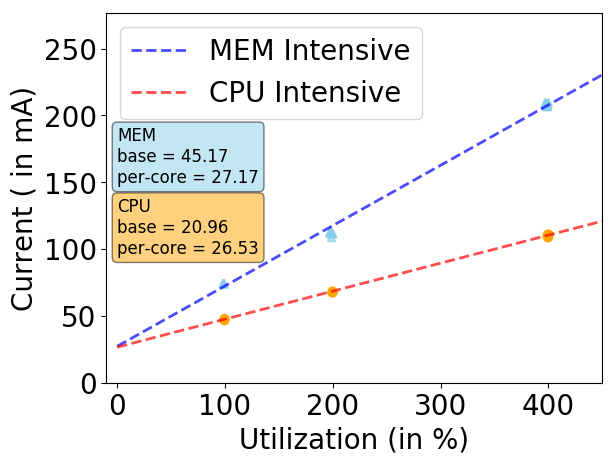
\includegraphics[width=\textwidth]{figures/576000.png}
         \caption{576 MHz}
         \label{fig:cpu_576000}
    \end{subfigure}
    \hfill
    \begin{subfigure}[b]{0.49\columnwidth}
         \centering
         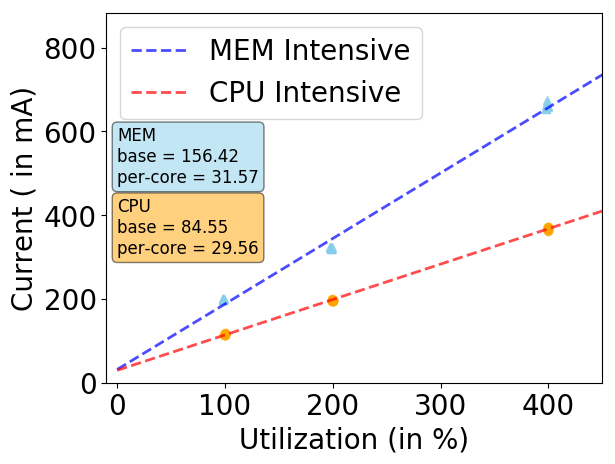
\includegraphics[width=\textwidth]{figures/1728000.png}
         \caption{1.728 GHz}
         \label{fig:cpu_1728000}
    \end{subfigure}
    \caption{The CPU derivation for two frequencies, 576 MHz and 1.728 GHz.}
    \label{fig:cpu_model_derivation}
    \vspace{-0.1in}
\end{figure}
\fi


\if 0
Figure~\ref{fig:cpu_model_derivation} shows 
the power consumed as a function of the CPU utilization for 576 MHz and 1.728 GHz,
for the two CPU benchmarks.
% While the blue line represents memory-intensive microbenchmark, red represents arithmetic-intensive microbenchmark .
% Figure~\ref{fig:cpu_576000} and~\ref{fig:cpu_1728000} corresponds to  576 MHz and 1.728 GHz
% Figure~\ref{fig:cpu_model_derivation} shows the power (averaged over 10 runs) linearly correlates with the utilization.
%% 3b. How model is derived
% We thus apply a regression-based solver to derive the best fit the following CPU power model:
% For each of the 31 frequencies, we derived a base and a per-core component with the following CPU power model.
% \begin{equation}
%     Power_{CPU}(f) = p_{base} + p_{f}*Utilization
% \end{equation}
% Where $p_{base}$ denotes the base power, and $p_{f}$ is the non-base per-core power running at frequency $f$.
%% 3c. Explain Base Current and Non-Base Current
For each of the 31 frequencies, we derived both base power and per-core component power.
We also observe that a reliable model can not be generated for the higher range of frequencies, like for frequencies higher than 2.035 GHz on MotoZ3 observations become unstable for CPU benchmarks.
The valid sets of base and per-core power were used for CPU modeling.
We observed that the base power is independent of frequency and per-core power is dependant on frequency.
Base power is 27.85 mA with a standard deviation of 1.22 mA.
% 
% We know the cores those are running at the 100\% utilization and remaining cores are offline.
% So, we can equate the number of running cores with utilization.
% We also observe that a reliable model can not be generated for the higher range of frequencies, like for frequencies higher than 2.035 GHz on MotoZ3 observations become unstable for CPU benchmarks.
% Fortunately, the apps rarely require these higher CPU frequency states and for our investigation we don't require those coefficients.
% \comment{stdev of what? fitting error on whole equation?}
% \comment{what is the following trying to say?}
During a  real run various cores may run on various frequencies.
\fi

\begin{figure}[tp]
    \centering
    \vspace{-0.1in}
         \begin{subfigure}[b]{0.49\columnwidth}
         \centering
    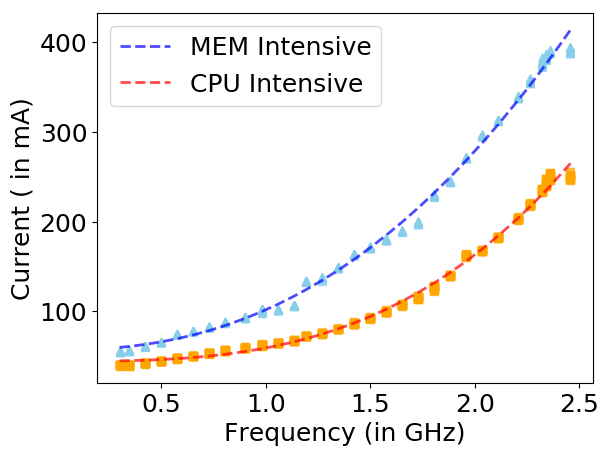
\includegraphics[width=\columnwidth]{figures/cpu_mem_characteristics.png}
    \caption{CPU power for compute-intensive vs. memory-intensive operations.}
    \label{fig:cpu_vs_mem}
\end{subfigure}
    \hfill
    \begin{subfigure}[b]{0.49\columnwidth}
         \centering
%    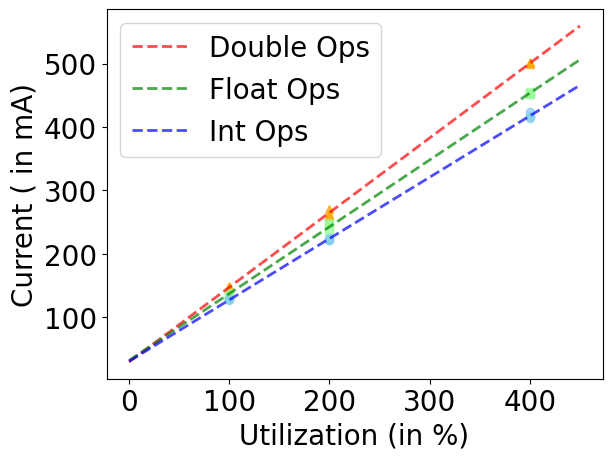
\includegraphics[width=\columnwidth]{figures/int_float_double.png}
    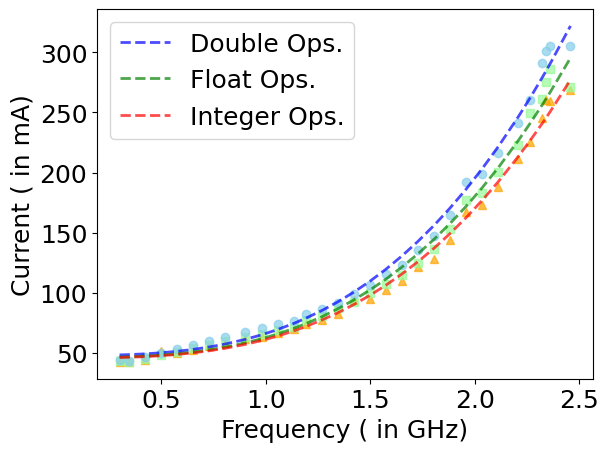
\includegraphics[width=\columnwidth]{figures/int_float_double_characteristics.png}
    \caption{CPU power for double, float and integer arithmetic operations.} % (for 1.8 GHz)}
    \label{fig:int_vs_float_vs_double}
    \end{subfigure}
    \caption{CPU power varies with app workload.}
    \label{fig:cpu_model_derivation}
    \vspace{-0.1in}
\end{figure}

\paragraph{Derived model}
Figure~\ref{fig:cpu_vs_mem} shows the derived CPU power model parameters
by plotting the total CPU power
as a function of the frequency.
% using the arithmetic-intensive and memory-intensive microbenchmarks. 
We observe that the CPU power draw for the two arithmetic-memory operation mix differ significantly,
by 38.7\% at the 300 MHz and 56.8\% at 2.45 GHz.
This suggests that the arithmetic-memory operation mix can send the CPU cores
to different power state variations draining different power.
In principle, this variation can be captured in the TPMD process by  
explicitly modeling memory as a separate phone component,
as in~\cite{carroll:2010,sesame:2011}, 
% gernot:2010 <- Koala: a platform for OS-level power management
using cache performance counter and free memory as the power triggers for memory draw. 
{
However, since the memory operation mix such as hardware counters is not collected by the mobile hardware 
or not reported by the Android OS on Android phones, it is much easier to lump memory power draw with CPU power draw as is commonly done in many recent work, including Android Battery Stats and Historian~\cite{androidbatterystats}. \comment{more example???}
}

Figure~\ref{fig:int_vs_float_vs_double} shows the derived CPU power model parameters for the integer only, 
float only, and double only arithmetic-intensive phases of the microbenchmark. 
We observe that the {CPU power} also differ, 
by 2.9\% at the 300 MHz and 13.5\% at 2.45 GHz.
This suggests that even the data type of arithmetic operations
can send the CPU cores into different power state variations.

\if 0
In summary, the above exercise of TPMD of CPU power shows the CPU power 
draw is very much app usage dependent and any fixed CPU model derived from
running a fixed microbenchmark is likely to have high estimation error when 
used in a particular app run. 
\fi


\if 0
\questionaj{This is not a very convincing argument. 1. For memory benchmark, is "CPU
power" = "CPU + memory" power? Or is the CPU power referenced in figure is true CPU 
power? If it is first, seeing higher "CPU power" is expected and not surprising.
2. Someone can argue that you could log memory triggers by instrumenting
compiler/libc/kernel,
why not just log?  Another paper didn't do it is not a strong reason. I think the 
argument we are trying to make is broader. That there are too many triggers that can 
affect a component power model. Because of which (a) micro-benchmark author may not 
know about all of them (b) building an exhaustive model could be expensive and not useful
as some model combinations may not even appear in real apps and (c) logging all 
triggers can be prohibitively expensive or not allowed. Because of this 
micro-benchmarks are hopelessly doomed.
If you agree,
we should also throw int-ops vs float-ops arithmetic, CPU temperature into the mix and use them to make the above three arguments.}
\fi
%\subsection{GPU Power Model is App Dependent}
\label{subsec:gpu}

Next, we show the GPU power model can also be highly dependent on app usage. 
The GPU gives an example of a component that cannot be exercised alone and we show
how TPMD models the GPU power incrementally over the CPU model.

%%% Things discussed in this section
%% 1. Explain GPU is complex in modern smartphones
%% 2. Explain the GPU frequencies and power states in modern smartphones
%% 3. Explain complete GPU model
%% 4. What did we do
%% 5. Explain results and observation
%%   5a. Explain per scenario dependent modeling
%%   5b. Explain the reasons for the observation

%The GPU of modern phones can run at various frequencies and transition among various power states.
\paragraph{Parameters of the GPU power model}
In Moto Z3, the GPU can run at 7 different frequencies and has three power states,
Active, Slumber (offline), and Aware.
When the GPU is woken out of the Slumber state, it enters the Aware state for a brief duration.
% \comment{Similarly, Nexus 6 can run at 5 different frequencies and three power states; Active, Init and Nap. Init corresponds to Aware and Nap corresponds to Slumber of Moto Z3}
%{
% How does does it stay in Aware?
%This the initialization phase of the GPU.
% for a fixed duration? 535 uS on average ( with a 250 uS difference between 435 uS (min) and 635 us (max))
% }
The Active state has two sub states, Active-busy when the GPU is computing and Active-idle
when the GPU is idle. After staying in Active-idle for a threshold interval, the GPU enters the Slumber state.
Since the GPU never enters the Slumber or Aware state when an app is running, 
the parameters of the GPU model include only the GPU power draw in Active-busy and Active-idle in each frequency, $p^g_{busy}(g_k), p^g_{idle}(g_k)$, as listed in Table~\ref{tab:parameters}.
We abbreviate Active-busy and Active-idle states simply
as GPU Busy and Idle states in the rest of the paper.

\if 0
Accordingly, we model the GPU power draw as follows:
\begin{equation}
    Power_{GPU} = \sum_{j}\sum_{i} u_{ij}*p_{ij}
    \end{equation}
where $p_{ij}$ is the power parameter for the $i^{th}$ GPU frequency for the $j^{th}$ power state (Active-busy, Active-idle, Slumber, Aware) and $u_{ij}$ is the corresponding utilization in that frequency and power state.
\fi

\paragraph{TPMD methodology}
% Similar to CPU, the GPU of modern smartphones have also vastly developed.
Initially, we tried to use a GPU benchmark, 3DMark~\cite{3DMark}, to drive the GPU usage into Busy and Idle states under each frequency.
However, we found that the GPU benchmark renders very different consecutive frames which
result in rapidly fluctuating GPU utilizations and power monitor readings.
This makes aligning the power monitor readings with the GPU Busy periods difficult
which is needed to extract the GPU Busy state power at each frequency.
%
% In power trace it was difficult to identify busy and idle traces for GPU benchmarks.This is because utilization is not constant as it continually generates new frames and can’t be paused.
% In apps the GPU utilization is constant because when no input is given to  the game app it generates the same frame again and again.
%
% we can only generate average GPU power coefficients for GPU busy and idle states.
% Average GPU coefficient depends on GPU utilization i.e  the time GPU is busy to total GPU running time.
%Average GPU power coefficients so derived is fixed and can not cater to two apps which may have different GPU utilization.
In contrast, we observe that real apps tend to render very similar consecutive frames in a short period of time which result relatively stable GPU utilization and stable GPU power draw, 
making it much easier to extract the power monitor reading corresponding to a given GPU utilization
(see Figure~\ref{fig:power_trace_candycrushturorial} later). 
%  the rendering task often finishes in less than the 16.7ms per-frame interval and hence the GPU will go through busy and idle states in every 16.7ms interval, making it much easier to manually identity both states. 
% \questionaj{Why do we have to identify manually? Triggers are not available in atrace?
% Due to both drift and scaling their is vast alignment problem in aligning each 16.7 ms interval.
% Alignment problem prevent us from directly using triggers from the event trace.}
Based on this observation, we directly used selected apps that use 
only the CPU and GPU to derive the GPU power models. 
In particular, we derive the CPU model first using the integer-arithmetic microbenchmark\footnote{We found using the CPU model derived using memory-intensive microbenchmark
resulted in negative GPU coefficients.}
and then use the difference 
between the measured phone power and model-estimated CPU power as the ground-truth for the GPU power draw
in GPU power model derivation.


% 5. Explain results and observation

\begin{table*}[tp]
{\footnotesize
    \centering
    \caption{Moto Z3 GPU power model (Busy and Idle power per frequency) with the CPU fixed at 1.056 GHz.}
    \vspace{-0.1in}
    \begin{tabular}{|p{11.5mm}|p{22mm}|c|c|c|c|c|c|c|c|c|c|c|c|c|c|}
    \hline
    App & Scenario & \multicolumn{14}{c|}{GPU Frequency} \\
    \cline{3-16}
     &  & \multicolumn{2}{c|}{257 MHz} & \multicolumn{2}{c|}{342 MHz} & \multicolumn{2}{c|}{414 MHz} & \multicolumn{2}{c|}{515 MHz} & \multicolumn{2}{c|}{596 MHz} & \multicolumn{2}{c|}{670 MHz} & \multicolumn{2}{c|}{710 MHz} \\
     \cline{3-16}
     & & Busy & Idle & Busy & Idle & Busy & Idle & Busy & Idle & Busy & Idle & Busy & Idle & Busy & Idle \\
    \hline
       \multirow{3}{11mm}{Boat Racing}  & Intro & 208.5 & 134.7 & 253.7 & 67.25 & 283.2 & 149.9 & 423.6 & 124.5 & 581.6 & 79.85 & 633.2 & 162.2 & 703.2 & 184.2 \\
       \cline{2-16}
        & Still & 232.3 & 145.5 & 358.0 & 57.00 & 402.8 & 153.0 & 573.9 & 92.17 & 576.3 & 150.0 & 813.9 & 145.0 & 866.3 & 205.9 \\
         
         & GPU engy. error (\%) & 232.3 & 145.5 & 358.0 & 57.00 & 402.8 & 153.0 & 573.9 & 92.17 & 576.3 & 150.0 & 813.9 & 145.0 & 866.3 & 205.9 \\
         
         \hline
        \multirow{2}{11mm}{Bricks Breaker}  & Intro & 140.7 & 70.33 & 158.3 & 69.32 & 204.3 & 109.9 & 166.8 & 134.4 & 130.0 & 141.3 & 115.5 & 172.9 & 133.2 & 191.4 \\
       \cline{2-16}
         & Still & 180.8 & 72.69 & 185.5 & 72.63 & 177.7 & 113.0 & 243.6 & 112.8 & 271.3 & 115.6 & 375.7 & 138.1 & 441.2 & 154.7 \\
         \hline
        \multirow{2}{13mm}{Candy Crush Saga}  & Into & 228.0 & 83.88 & 262.5 & 83.97 & 344.4 & 112.7 & 523.1 & 123.3 & 620.7 & 120.0 & 792.6 & 146.2 & 900.4 & 167.2 \\
        \cline{2-16}
         & Tutorial & 226.3 & 92.85 & 228.4 & 89.50 & 330.6 & 117.7 & 445.2 & 134.5 & 519.6 & 137.5 & 660.2 & 160.7 & 855.3 & 171.6 \\
         \hline
    \end{tabular}
    \label{tab:gpumodel_motoz3}
    \vspace{-0.1in}
    }
\end{table*}

% Comparison Table for GPU model with other scenarios Here

We repeated the GPU model derivation for three
popular games apps, Boat Racing, Candy Crush Saga and Bricks breaker.
each running two scenarios, as listed in Table~\ref{tab:app_scenario_description}.
To minimize the variance of CPU power draw, we fixed the CPU frequency at 1.056 GHz,
and ran each app scenario under each GPU frequency for a duration of 60 seconds.

\paragraph{Derived model}
Table~\ref{tab:gpumodel_motoz3} shows the derived GPU power models for varying GPU frequencies for Moto Z3 and Table~\ref{tab:gpumodel_nexus6} for Nexus 6.
%% 5a. Explain per scenario dependent modeling
We make two observations.
(1) The GPU power parameters for the same frequency differ with {\it different apps}; at 710 MHz, the GPU Busy power draw for Boat Racing is 10.6\% lower than for Candy Crush Saga on Moto Z3.
(2) The GPU parameters for the same frequency even differ for {\it different scenarios} 
of the same app; for Boat Racing, the GPU Busy power draw
for the Intro scenario is 10.2\% and 29.7\% lower than for the Still scenario
at 257 MHz and 414 MHz, respectively.

To show the importance of app-specific power modeling, we calculated the error
in estimating the total GPU energy drain in the second scenario of each app 
if using the GPU model derived using the first scenario of each app.
Table~\ref{tab:gpumodel_motoz3} shows that the error ranges between 
??\%--??\%, ??\%--??\%, and ??\%--??\% for the second scenarios of the three apps.


%% 5b. Explain the reasons for the observation
The above dependence of the GPU power draw on app usage can be attributed  to two main reasons.
First, the GPU has a large number of mini-cores, but the utilization metric available to the OS only captures the temporal utilization but not the spatial utilization, \ie the percentage of mini-cores that were active.
Different spatial utilization may drive the GPU into different power state variations that have the same temporal utilization but different power draw.

Second, rendering different frames in different scenarios of the same app or different apps may result in different memory operation mix, and hence using a single CPU model in estimating the CPU power draw portion to be subtracted from the total phone power 
may result in errors in the GPU power draw  estimation, as we see in \S\ref{sec:primer_cpu}. 
Such error propagation happens in TPMD which models one component at a time
and often relies on the models for prior components to estimate the "ground truth" in modeling  the next component. 

\subsection{TPMD is labour intensive}

\paragraph{Designing microbenchmarks} 
We start the process of TPMD by first identifying the list of {\it power model parameters}
for CPU and GPU, as listed in Table~\ref{tab:parameters}.
% \paragraph{Parameters of the CPU and GPU power models.}
% Pixel2, Moto Z3~\cite{motoz3} and Pixel 4 are representative of modern smartphones
% that uses the big.LITTLE CPU architecture~\cite{biglittlearch} to
% provide energy efficiency in supporting diverse workloads.
% Particularly, in Pixel 2 and Moto Z3, the LITTLE cores can operate in 22 different frequencies 
% and big cores can operate in 31 different frequencies.
% Whereas, for Pixel 4, the LITTLE cores can operate in 18 different frequencies 
% and big cores can operate in 20 different frequencies.
%  The cores are switched to higher frequencies when higher performance is required.
% At runtime, the OS scheduler along with the CPU governor performs power state transition and core frequency scaling to optimize the CPU energy draw as the workload varies.
From~\cite{multicoremodel:2015}, the parameters of the CPU power model include
the base power consumed $p_{\text{base}}$ when the cores are idle and
the non-base core $i$ power running at frequency $f_k$, $p^c_i(f_k)$.
%, as listed in Table~\ref{tab:parameters}.
% The total CPU power can be modeled as:
% {
% \begin{equation}
%     P_{\text{CPU}} = p^c_{\text{base}} + \sum_{i} p^c_i(f_k)
% \end{equation}
% 
% }
% In Moto Z3, 
% GPU can run at different frequencies and can either be busy or idle.
% has three power states, Active, Slumber, and Aware.
% Since the GPU never enters the Slumber or Aware state when an app is running, 
The parameters of the GPU model include the GPU power draw in 
% Active-busy and Active-idle 
busy and idle states in each frequency, $p^g_{\text{busy}}(g_k)$ and 
$p^g_{\text{idle}}(g_k)$.
% We abbreviate Active-busy and Active-idle states simply
% as GPU Busy and Idle states in the rest of the paper.

% \if 0
% Accordingly, we model the GPU power draw as follows:
% \begin{equation}
%     Power_{GPU} = \sum_{j}\sum_{i} u_{ij}*p_{ij}
%     \end{equation}
% where $p_{ij}$ is the power parameter for the $i^{th}$ GPU frequency for the $j^{th}$ power state (Active-busy, Active-idle, Slumber, Aware) and $u_{ij}$ is the corresponding utilization in that frequency and power state.
% \fi

%\paragraph{TPMD methodology.}
We design CPU microbenchmarks that perform 
arithmetic and memory operations for 7 seconds each 
with 100\% utilization.

\begin{sloppy}
For the GPU, we first used a third-party rendering benchmark 3DMark~\cite{3DMark}. 
	But on running the benchmark, we found that 3DMark renders quite different
	consecutive frames which result in rapidly fluctuating GPU utilizations and
	power monitor readings, making the alignment \comment{of what?? of
	the 16.7 ms GPU rendering intervals wrt the power monitor as each rame has a different GPU utilization} difficult. 
\end{sloppy}
In contrast, we observed that real apps tend to render very similar consecutive
frames in a short period of time which result in relatively stable GPU
utilization and stable total power draw, making it easier to extract the power
monitor reading corresponding to a given GPU utilization (see
Figure~\ref{fig:power_trace_candycrush_menu} later).  Thus, we directly used
selected apps that use only the CPU and GPU to derive the GPU power models.  In
particular, we derive the CPU model by first using the 
% integer-arithmetic 
CPU arithmetic microbenchmark\footnote{We found using the CPU model derived
using memory-intensive microbenchmark resulted in negative GPU coefficients.}
and then using the difference between the measured phone power and
model-estimated CPU power when running an app as the ground-truth for the GPU
power draw and GPU power model derivation.


\paragraph{Running microbenchmarks}
\aj{We first prepared the three phones by connecting power monitor and bypassing 
the battery interface.} \comment{Were there some challenges here for separate 
device models?}
\dcomment {
We faced different challenges while attaching each device to the power monitor
\eg attaching the power monitor leads to power management circuit .
}

We ran the CPU microbenchmark while fixing the big core cluster at each 
of the 31 frequencies
for both Pixel 2 and Moto Z3 and at each of the 20 frequencies for Pixel 4, 
on 1 core and 2 cores.
% When using 1 core, 2 cores and 4 cores, the remaining cores are offline.
We measure the base CPU power as the phone power draw when all cores are idle.
We manually align the power monitor readings for each of the 7-second interval 
and derive the non-base per-core power for each frequency by 
subtracting the base power from the measured total phone power.
\comment{This is not bad? Only (7+7)*31 = ~7 minutes of run. Do we have to repeat
it multiple times or something else that makes it LABORIOUS?
}
\dcomment{
For the purpose for this paper we considered only 2 big cores for the ease of our experiments.
While in the real world scenario the device has to profiled on all states \ie
taking into account the interaction between the LITTLE core and big cores.
There are in total 24 configuration of cores for Pixel 2 in which they can be
online ( for a 4 LITTLE cores 0 to 4 cores could be active, same for big cores,
remove the case where both cores are offline).
As there are 22 LITTLE core and 31 big core frequencies we further have $22x31=682$
combination. Using our methodology it could take up to $24x682x7$ seconds = 1.33 days for
just to gather the required measurements.
}
% After running
% the benchmarks, we found that for all the
% phones, 
% %we found that 
% the per-core power $p_i(f_k)$ remains the same for different cores.

% Similar to CPU, the GPU of modern smartphones have also vastly developed.
% Initially, we tried to use a GPU benchmark, 3DMark~\cite{3DMark}, to drive the GPU usage into Busy and Idle states under each frequency.
%
% This makes aligning the power monitor readings with the GPU Busy periods difficult
% which is needed to extract the GPU Busy state power at each frequency.
%
%  the rendering task often finishes in less than the 16.7ms per-frame interval and hence the GPU will go through busy and idle states in every 16.7ms interval, making it much easier to manually identity both states. 
% \questionaj{Why do we have to identify manually? Triggers are not available in atrace?
% Due to both drift and scaling their is vast alignment problem in aligning each 16.7 ms interval.
% Alignment problem prevent us from directly using triggers from the event trace.}

% 5. Explain results and observation

\begin{figure*}[tp]
    \centering
     \begin{subfigure}[b]{0.32\textwidth}
         \centering
         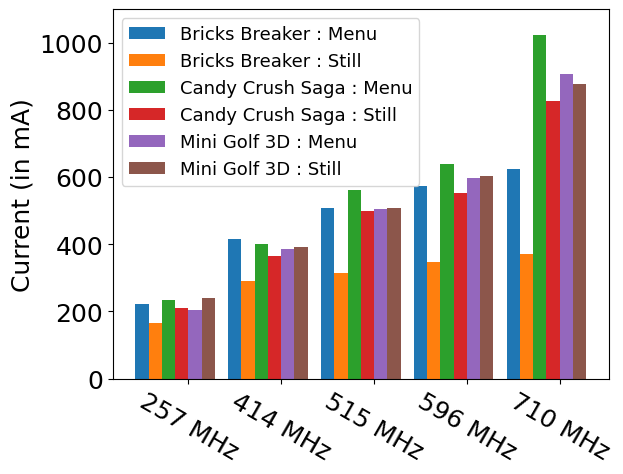
\includegraphics[width=\textwidth]{figures/002_Pixel2_gpu_model.png}
         \caption{Pixel 2}
         \label{fig:gpu_model_p2}
     \end{subfigure}
    \begin{subfigure}[b]{0.32\textwidth}
         \centering
         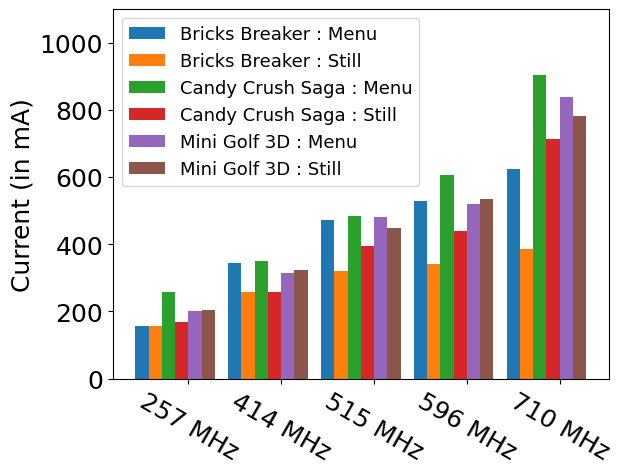
\includegraphics[width=\textwidth]{figures/003_MotoZ3_gpu_model.png}
         \caption{Moto Z3}
         \label{fig:gpu_model_z3}
     \end{subfigure}
    \begin{subfigure}[b]{0.32\textwidth}
         \centering
         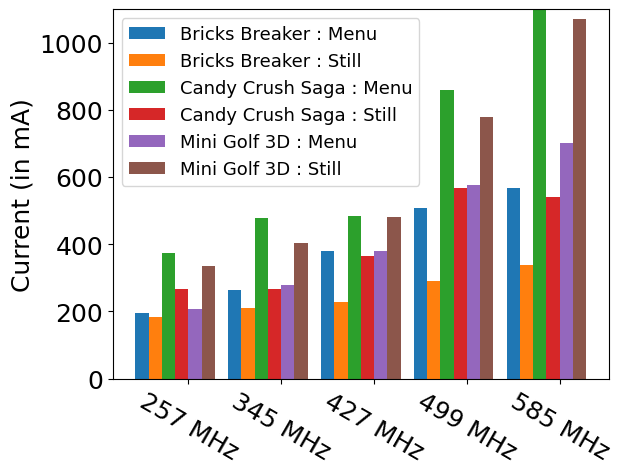
\includegraphics[width=\textwidth]{figures/004_Pixel4_gpu_model.png}
         \caption{Pixel 4}
         \label{fig:gpu_model_p4}
     \end{subfigure}
     \hfill
    \caption{TPMD-derived GPU power model (only Busy power is shown) with
        the CPU frequency fixed at 1.42 GHz for both Pixel 2 and Moto Z3,
        and 1.61 GHz for Pixel 4. ??? FIXED}
    \label{fig:gpu_model}
    \vspace{-0.1in}
\end{figure*}

\begin{table*}[tb]
    \caption{Energy estimation error (\%) for app scenarios 
    using the GPU model derived for each scenario with CPU and GPU frequencies fixed for the 3 phones. (B: Bricks Breaker, C: Candy Crush Saga and M: Mini Golf 3D)}
    \vspace{-0.1in}
    \centering
    \begin{subfigure}[b]{0.31\textwidth}
        \caption{Pixel 2}
        \vspace{-0.05in}
        \centering
    	{ \scriptsize
    	\begin{tabular}{ | p{10.8mm} | c | c | c | c | c | c | }
    		\hline
    		     & \multicolumn{6}{ c|}{Error for each App Sc. (\%)}\\ % \multicolumn{6}{ c|}{Error for each App Scenarios (\%)}\\
    		\cline{2-7}
                    Model & \rot{B. Menu} & \rot{B. Still} & \rot{C. Menu} & \rot{C. Still} & \rot{M. Menu} & \rot{M. Still}  \\
    		\hline
                B. Menu              & 8.9 & 13 & 20 & 16 & 11 & 14 \\
                B. Still             & 15 & 11 & 31 & 25 & 17 & 26 \\
                C. Menu              & 16 & 24 & 11 & 11 & 13 & 11 \\
                C. Still             & 16 & 19 & 14 & 12 & 12 & 14 \\
                M. Menu              & 9.9 & 14 & 14 & 11 & 8.1 & 11 \\
                M. Still             & 12 & 21 & 9.7 & 10 & 11 & 8.6 \\
    		\hline
    	\end{tabular}
    	}
    \end{subfigure}
    \hfill
    \begin{subfigure}[b]{0.31\textwidth}
        \caption{Moto Z3}
        \vspace{-0.05in}
        \centering
    	{ \scriptsize
    	\begin{tabular}{ | p{10.8mm} | c | c | c | c | c | c | }
    		\hline
    		     & \multicolumn{6}{ c|}{Error for each App Sc. (\%)}\\ % \multicolumn{6}{ c|}{Error for each App Scenarios (\%)}\\
    		\cline{2-7}
                    Model & \rot{B. Menu} & \rot{B. Still} & \rot{C. Menu} & \rot{C. Still} & \rot{M. Menu} & \rot{M. Still}  \\
    		\hline
                B. Menu              & 16 & 18 & 44 & 18 & 22 & 25 \\
                B. Still             & 18 & 15 & 36 & 15 & 17 & 17 \\
                C. Menu              & 30 & 24 & 16 & 23 & 18 & 16 \\
                C. Still             & 12 & 12 & 31 & 11 & 15 & 17 \\
                M. Menu              & 18 & 16 & 23 & 15 & 14 & 15 \\
                M. Still             & 20 & 15 & 20 & 14 & 12 & 13 \\
    		\hline
    	\end{tabular}
    	}
    \end{subfigure}
    \hfill
    \begin{subfigure}[b]{0.31\textwidth}
        \caption{Pixel 4}
        \vspace{-0.05in}
        \centering
    	{ \scriptsize
    	\begin{tabular}{ | p{10.8mm} | c | c | c | c | c | c | }
    		\hline
    		     & \multicolumn{6}{ c|}{Error for each App Sc. (\%)}\\ % \multicolumn{6}{ c|}{Error for each App Scenarios (\%)}\\
    		\cline{2-7}
                    Model & \rot{B. Menu} & \rot{B. Still} & \rot{C. Menu} & \rot{C. Still} & \rot{M. Menu} & \rot{M. Still}  \\
    		\hline
                B. Menu              & 15 & 15 & 44 & 19 & 15 & 34 \\
                B. Still             & 15 & 15 & 50 & 23 & 17 & 40 \\
                C. Menu              & 30 & 33 & 12 & 20 & 25 & 13 \\
                C. Still             & 18 & 20 & 25 & 15 & 16 & 19 \\
                M. Menu              & 15 & 16 & 34 & 17 & 14 & 26 \\
                M. Still             & 25 & 28 & 13 & 15 & 21 & 12 \\
    		\hline
    	\end{tabular}
    	}
    \end{subfigure}
    \label{tab:gpu_model_error}
    \vspace{-0.1in}
\end{table*}
% Comparison Table for GPU model with other scenarios Here

For GPU model derivation, we repeated runs for three popular games apps,
Bricks Breaker, Candy Crush Saga and Mini Golf 3D, each running two
scenarios, as listed in Table~\ref{tab:app_scenario_description}.  To
minimize the variance of CPU power draw, we fixed the CPU frequency at
1.42 GHz for both Pixel 2 and Moto Z3, and 1.61 GHz for Pixel 4, and ran
each of the app scenario under each GPU frequency for a duration of 30
seconds.
\comment{Again, not not bad. What makes this process LABORIOUS?}
\dcomment {
The GPU model derivation has to be derived for each app the user requires.
Making this impossible to device manufactures to model GPU in it entirely
as there are billions of apps presents currently.
}

\subsection{TPMD is not comprehensive}

Our CPU modeling results (details omitted) show that
the CPU power draw for the arithmetic-intensive and memory-intensive
operations of the microbenchmark differ significantly,
by 38.7\% at 300 MHz and 56.8\% at 2.45 GHz for Moto Z3.
This suggests that the arithmetic-memory operation mix can send the CPU cores
to different power state variations, draining different amount of power.

Figure~\ref{fig:gpu_model}(a)-(c) shows the derived power models 
for varying GPU frequencies for the 3 phones. 
Only GPU Busy power are shown due to page limit.
% The full bars represent the busy current whereas the solid bars are the idle current.
% and Table~\ref{tab:gpumodel_nexus6} for Nexus 6.
%% 5a. Explain per scenario dependent modeling
We make two observations.
%
(1) The GPU power parameters for the same frequency differ with {\it
different apps}. For example, on Moto Z3 at 710 MHz, the GPU Busy power draw for
Bricks Breaker Still is 57.2\% lower than for Candy Crush Saga Menu.
%
(2) The GPU power parameters for the same frequency even differ for
{\it different scenarios} of the same app. For example, for Bricks Breaker, the GPU
Busy power draw for the Still scenario is 32.3\% and 35.5\% lower than
for the Menu scenario at 515 MHz and 596 MHz, respectively, on Moto Z3.
Similar observations can be made about the other two phones.

%% 5b. Explain the reasons for the observation
The above dependence of the GPU power draw on app usage can be
attributed to two main reasons.  (1) The GPU has a large number of
mini-cores, but the utilization metric available to the OS only
captures the temporal utilization and not the spatial utilization, \ie
the percentage of mini-cores those were active.  Different spatial
utilization may drive the GPU into different power state variations
that have the same temporal utilization but different power draw.
% 
(2) Using a single CPU model in estimating the CPU power draw which is
 to be subtracted from the total phone power may result in errors in
 the GPU power draw estimation, as rendering different frames for
 different app scenarios (of the same or different apps) may result in
 different CPU usage, \eg due to different mix of arithmetic and
 memory operations and hence CPU power draw.  Such error propagation
 happens in TPMD which models one component at a time and often relies
 on the models of a prior component to estimate the "ground truth" in
 modeling the next component.

% \paragraph{Cross validation.}
To further demonstrate that the GPU models derived per app scenario captures
the model dependence on the app usage also, we perform a cross validation
by applying the GPU model derived from each of the six app scenarios
shown in Figure~\ref{fig:gpu_model}(a)-(c) to estimate the total
energy of all app scenarios (including self).
Tables~\ref{tab:gpu_model_error}(a)-(c) shows the results for 
the case where the CPU frequency is fixed at 1.42 GHz for Pixel 2 and Moto Z3 and 1.61 GHz for Pixel 4, and the GPU frequency is fixed at 257 MHz for all three phones.
We observe that the energy estimation error
is much lower when the GPU model derived for an app scenario is
applied to itself (diagonal values), ranging between 
8.09\%-11.56\% for Pixel 2,
11.47\%-16.25\% for Moto Z3, and
11.90\%-15.21\% for Pixel 4,
than when a model derived for one scenario is applied
to other scenarios (off-diagonal values), which
range between 
9.73\%-31.26\%,
11.57\%-44.25\%, and
13.07\%-50.43\%.


% \comment{
% We observe that the lowest error for a scenario is
% due to GPU model derived from same scenario (fitting error), whereas for
% all other scenario GPU models the error can be as much as 2$times$ higher.
% For the higher GPU frequencies, like 710 MHz the difference in the can increase up to about 10 times.
% }


\if 0
we calculated the error
in estimating the total GPU energy drain in the second scenario of each app 
if using the GPU model derived using the first scenario of each app.
The rows labelled "GPU energy error" in Table~\ref{tab:gpumodel_motoz3} shows that the error ranges between ??\%--??\%, ??\%--??\%, and ??\%--??\% for the second scenarios of the three apps.
\fi







\paragraph{Summary.}
The above exercise of applying TPMD to derive the CPU and GPU models for 3 phones
have two important implications.
%
(1) TPMD is a laborious time-consuming process. In-situ power modeling
such as done by SPMD will enable rapid portability of energy related software.
(2) The GPU power draw is very much dependent on app usage; different
app usage can lead to variations of the same power state that draw
different amount of power. Hence {\it any fixed GPU model derived from
running a particular microbenchmark or app is likely to have high
estimation error when it is applied for a different app run.} This
motivates the need for SPMD which is inherently app usage specific.
%
\comment{(3) Don't think this should be here. This section is about TPMD. Find where to
move it.
Since different scenarios of the same app can drive components
into different power state variations, {\it the equations from
different scenarios of the same app run should not be grouped into the
same system of equations to be fed into the solver in SPMD,} as this
defeats the app usage specificity nature of SPMD.}


\section{Self Power Modeling Methodology}
\label{sec:method}

In this section, we first describe the basic self power modeling
methodology. We then discuss a set of practical challenges in applying
SPMD  and how we address them:
(1) How to set up the system of equations?
(2) How to constrain the solver to make it output meaningful models?
(3) How to validate the SPMD-derive models?
(4) Are built-in power sensors accurate enough for use in SPMD?

\if 0
present a set of constraints that we add to the
basic solver to help the solver to output meaningful model parameters.
and for the usabiity of Android phones power sensor readings.
\fi

% as depicted in Figure~\ref{fig:equations}.
\if 0
\begin{figure}[tp]
    \centering
    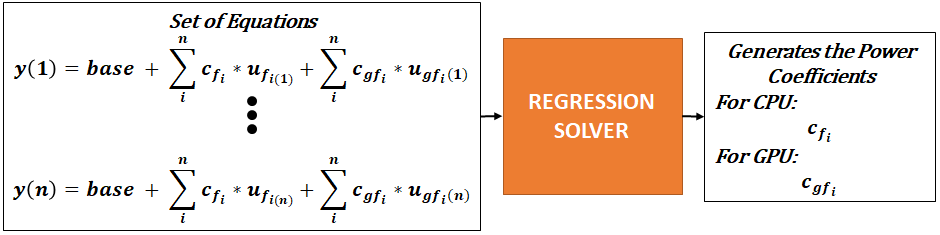
\includegraphics[width=0.95\columnwidth]{figures/design_2.png}
    \vspace{-0.1in}
    \caption{SPMD via solving a system of linear equations.}
    \label{fig:equations}
    \vspace{-0.1in}
\end{figure}
\fi

\begin{table}[t]
{\footnotesize
    \centering
    \caption{Power state, utilization, and energy collected during online app run.}
    \vspace{-0.1in}
   % \begin{tabular}{|p{32mm}|p{10mm}|p{23mm}|}
    \begin{tabular}{|l|P{11mm}|c|}
    \hline
          &  Symbol & Collection method \\
         \hline
         \multicolumn{1}{|l|}{\textbf{Power State}} &  &   \\
         CPU Frequency      & $f_{k}$                               & cpu\_frequency \\
         GPU Frequency      & $g_{k}$                               & kgsl\_pwrlevel \\
         GPU State          & $s_j$                                 & kgsl\_pwr\_set\_state \\
         \hline
          \multicolumn{1}{|l|}{\textbf{Utilization}} &   &  \\
         
         \multicolumn{1}{|l|}{CPU Util. in freq. $f_k$}               & $u^c(f_{k})$        & cpu\_idle \\
         \multicolumn{1}{|l|}{GPU Util. in freq. $g_k$,}  & $u^g(g_k,s_j)$      & kgsl\_pwrstats \\
          \mbox{\hspace{0.6in}}state $s_j$ & & \\
         \hline
         \multicolumn{1}{|l|}{Energy drain}     & $y$                                &
         \multicolumn{1}{p{30mm}|}{/sys/class/power\_supply /charge\_counter} \\
         \hline
    \end{tabular}
    \label{tab:triggers}
    \vspace{-0.2in}
}
\end{table}

\subsection{Basic SPMD Process}
\label{subsec:generic}

As discussed in \S\ref{subsec:spmd}, SPMD consists of two basic steps: 
\dcomment{(1)} online data collection for setting up a system of equations and 
\dcomment{(2)} offline model derivation by solving the system of equations.

\paragraph{Online data collection.}
Since SPMD is "in-situ", we need to collect the data needed to set up the
equations while the app is running.
% As discussed in \S\ref{sec:primer}, in modern phones, the CPU and GPU power draw are 
% functions of the operating frequency and the power state (for GPU). Therefore,
% for power triggers, we need to collect the duration each component spends in every 
% combination of frequency and power-state during the app run, as listed in Table~\ref{tab:triggers}.
%
Table~\ref{tab:triggers} lists the data that need to be collected and
how they are collected on Android phones.  The data include the power
states and utilization in each state of each component used by the
app,
%  for each time interval corresponding to an equation 
as well as the whole-phone power draw or energy drain,
\eg in every small time interval during app run.

We use the Linux event trace~\cite{eventtrace} to collect the power
state and utilization.  To collect whole-phone energy draw per
time interval, we can use either the built-in power sensor energy counter
which became available since Android {7}, or an external power
monitor such as Monsoon~\cite{monsoonpowermonitor}.

\cut{ Ideally, reading from the built-in power sensor is preferred,
  since it does not require wiring the phone battery and potentially
  allows SPMD to be performed on any phones, including users' phones
  "in the wild". However, as we will see in the next section, built-in
  power sensor readings have such high error that makes them
  impractical to use in SPMD.  }

\if 0
\begin{figure}[tp]
{\small
    \centering
    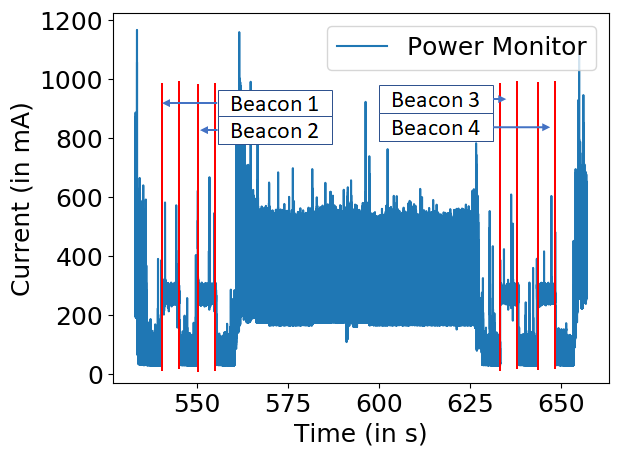
\includegraphics[width=0.80\columnwidth]{figures/beacons_3.png}
    \vspace{-0.1in}
    \caption{Beacons to align power monitor with phone clock.}
    \label{fig:align_beacon}
    \vspace{-0.1in}
}
\end{figure}
\fi

%%%%%%%%%%%%%%%
\paragraph{Offline model derivation.} 
%
% In offline processing, \eg 
When the app run finishes, SPMD sets up a system of linear
equations with the phone component power parameters as unknowns.  In
general, the trace duration is cut into $K$ equal intervals of $T$
seconds each, and one equation is created for interval $t$ as follows:
\begin{align}
y_t = p^{c}_{\text{base}} +& \sum_i\sum_k{u^c_t(f_k)p_i^{c}(f_{k})} + \nonumber \\
        & \sum_{j}\sum_{k} u^g_t(g_k,s_j)p^{g}(g_k, s_j)
\end{align}
where the double summation for the CPU is over all the CPU cores and frequencies,
the double summation for the GPU is over all the GPU frequencies and GPU states,
$u^c_t(f_k)$ and $u^g_t(g_k,s_j)$ are the CPU and GPU utilization for the corresponding power states
in time interval $k$,
and the left-hand-side (LHS) $y_t$ is the total phone energy drain in time interval $t$.
% where model parameter $p^c(f_{i})$ is the CPU power draw for frequency $f_i$,  
% model parameter $p^g_{ij}$ is the GPU power draw at frequency $f_i$ and power state $j$, the utilization coefficients $_{f_{i}}(k)$ and $u_{ij}(k)$ equal the total utilization (in seconds) of CPU and GPU in the corresponding frequencies and power states in the $k$th trace interval, and $y(k)$ denotes the total phone energy drain during interval $k$ from integrating power sensor or power monitor readings.
% \cut{ 
% Clearly, in a given app run, the CPU and GPU may not go through all possible frequencies and power states, and hence not all power parameters may show up in the equations. SPMD will only derive those power model
% parameters actually encountered in the app run. This is not an issue with SPMD as only those parameters will be needed for the power model applications such as energy profiling or energy debugging. 
% }
\st{Since there can be more equations than the number of unknowns, 
the system of equations can be solved using a regression-based
solver to generate the power parameters.} In this paper, we use
the python curve\_fit() function which uses {\color{blue}the}
\dcomment{non-linear}
least square fitting as our regression solver~\cite{curvefit}.

Notice that although SPMD via solving a system of equations using a regression solver is
conceptually simple{\color{blue}, due to the existence of noise in measurement, the modeling results from linear regression solver could be invalid. Further, different setup will affect the final modeling results. Therefore, it is worthwhile to examine the modeling quality of SPMD under different settings and understand why SPMD works or not with certain setup.}

\if 0
\subsection{SPMD Challenges}
\label{subsec:challenges}

SPMD via solving a system of equations using a regression solver is conceptually simple. 
In practice, the single biggest challenge is whether the system of equations 
has enough diversity so that the regression solver
can generate meaningful solutions to the system, \ie power model parameters. 
The answer is not obvious for at least two reasons.

{\bf Condition 1: Usage coefficients lack diversity.}
First, \S\ref{sec:primer} has concluded that
we need to set up a system of equations for each app scenario as different scenarios
even of the same app can have different component usage. However, 
one can imagine that the app behavior for the same app scenario may be highly repetitive and hence
the resulting equations, either the usage terms on one side or the energy drain on the other side,
 may look similar or only differ slightly, resulting on low rank of the equations. 

{\bf Condition 2:s Noisy energy measurement.}
The energy measurement can contain noise and if the difference among the true energy values for different equations is small, the noise level may dominate the energy variations of the different equations. This can result in the regression solver trying to minimize the fitting error from noisy energy measurement as opposed to fitting the true energy difference.  

Our verification study centers around addressing this challenge, by systematically exploring different ways of setting the system of equations to try to increase the diversity.

Before presenting our verification study, we discuss two refinements we added
to the basic SPMD methodology.


\fi

\subsection{How to Set up Equations?}
\label{subsec:howtosetup}

The basic SPMD methodology does not specify how to set up systems of
equations for the regression solver for a given app run. Since SPMD is
"in-situ", \ie it derives all the power model parameters experienced
during a given app run, in principle we need to create equations that
cover the entire app run duration.  Given an app run of duration
$T$, we can potentially chop it into $N_s$ equal-sized epochs, and
set up $N_e$ equations per each epoch, each covering a duration of
$t_e$ of the app run, \ie
\begin{eqnarray}
T = N_s \cdot N_e \cdot t_e
\end{eqnarray}
%
Thus, setting equations for SPMD has two degrees of freedom: 
(1) How many systems of equations $N_s$ shall we create for an app run? 
(2) How many equations $N_e$ shall we create for each epoch?
Our verification study explores how the two degrees of freedom can 
help us \st{to improve the diversity for the systems of equations.}{\color{blue} to get valid modeling results.}

\subsection{Adding Constraints to the Solver}
\label{subsec:constraint}

As we will see in \S\ref{sec:modelling_macro}, because the regression
solver tries to minimize the fitting error and is oblivious to the
semantics of the unknowns, it may output solutions that minimize the
fitting error but violate basic properties of the power model
parameter values, such as non-negativity {\color{blue}(all coefficients should not be negative)} and monotonicity {\color{blue}(coefficients of higher frequency should be larger)}.  To overcome
this, in addition to the basic unconstrained regression solver, {\color{blue}we also experimented two constrained regression solver} based on the domain knowledge of power models, as shown in
Table~\ref{tab:constrained}.

\begin{table}[tp]
%\questionaj{These constraints must also constrain GPU busy and idle.}
{\small
    \centering
    \caption{Constraints added to the regression solver.}
    \vspace{-0.1in}
    \begin{tabular}{|p{25mm}|p{52mm}|}
    \hline
         Constrained SPMD  & \multicolumn{1}{c|}{Description} \\
         \hline
\hline
         Unconstrained      & No constraints are applied. \\
\hline
         Constrained        & Model parameters should not decrease with increasing frequencies. GPU idle power is less than GPU busy power. \\
\hline
         Freq-constrained   & CPU model parameters are modeled as a polynomial of frequency. \\
         \hline
    \end{tabular}
    \label{tab:constrained}
    \vspace{-0.1in}
}
\end{table}


\paragraph{Constraint 1: positivity and monotonicity.}
Without any constraint, we found the regression solver can output
CPU/GPU power values that are negative or decreasing when the
frequency increases.  To prevent the solver from outputing such
solutions, we added three constraints to the regression solver: (1) all
model parameters should be positive; (2) the model parameters with
increasing frequencies for each component should be non-decreasing;
(3) the GPU Idle power should be lower than the GPU Busy power.  We
denote this version of SPMD as "Constrained SPMD".


\paragraph{Constraint 2: modeling CPU power as a function of frequency.}
We found even with Constraint 1, the CPU power parameters with varying
frequencies output by the solver often remain the same.  To make the
CPU model parameters output more consistent with the reality, we
exploited another domain knowledge about the CPU power draw, that it
increases as a low-order polynomial of the operating
frequency~\cite{armdvfs,rizvandi2011some}.
% Since the specific polynomial function may vary for different phones, \eg early phones only performed % frequency scaling (FS) while newer phones perform dynamic voltage and frequency scaling (DVFS), we first used a simple CPU benchmark to find the order of the polynomial for each phone used in our experiments. 
%
\if 0
\begin{figure}[tp]
    \centering
%    \vspace{-0.1in}
    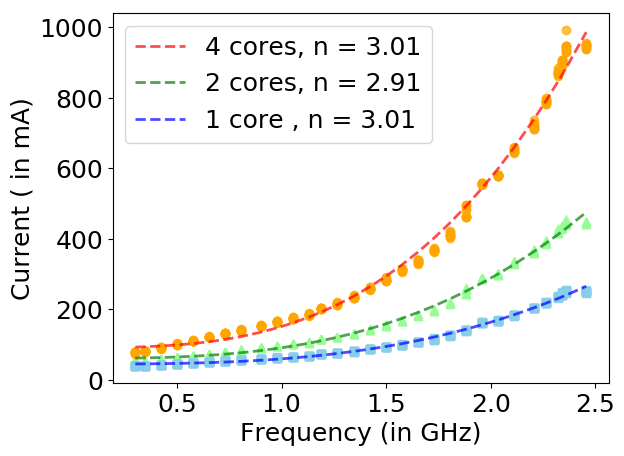
\includegraphics[width=0.80\columnwidth]{figures/cpu_characteristics.png}
    \caption{Moto Z3 big core CPU power draw grows with frequency 
    when running the arithmetic-intensive benchmark.}
    \label{fig:cpu_characteristic}
    \vspace{-0.1in}
\end{figure}
\fi
%
\cut{ We ran a microbenchmark that performs arithmetic-intensive or memory-intensive operations for 7 seconds
on 1, 2 and 4 big cores, for each big core frequency, and fit the measured phone power 
with a polynomial function in frequency.
%\begin{equation}
%     P_{CPU} = p^c_{base}+ \sum_i p^c_i({f_k}) = p_{base}+\sum_i  a*f_k^{n}
% \end{equation}
% Figure~\ref{fig:cpu_characteristic} shows the measured power draw and curve fitting on Moto Z3.
}
Our CPU microbenchmark results show  that 
% the fitted exponent $n$ for 1, 2 and 4 cores are 3.01, 2.97 and 3.01, respectively.
the per-core power grows as the third-power of the CPU
frequency on all three phones, 
\ie $p_i^c(f_k) = a\cdot f_k^3$. 
Thus we replace all the CPU power parameters with
third-power of the CPU frequency in the SPMD model equations.
%model the Moto Z3 big core power as a third-order polynomial of the CPU frequency in the model equations of SPMD.
%
Doing so has two benefits: (1) it reduces the number of CPU power
parameters from $K$, the number of CPU frequencies, to 2, the base power $p_{\text{base}}$
and coefficient $a$, which reduces the number of equations needed for
the solver; (2) it constraints the CPU power to be not only
monotonically increasing with its frequency, but also consistent with its physical power behavior.


%%%%%%%
\subsection{How to Validate Modeling Results from SPMD?}
\label{subsec:validate}

{\color{blue}Because SPMD aims to generate different modeling results for different scenarios, it is unreasonable to use measurements from other app runs to test our modeling results for a specific app run. However, since we have already assume that the ground truth is a linear model, we only need to verify that whether the output of the linear regression is validate or not. In the field of statistical learning, F-test and $R^2$-measurement are commonly used to validate the effectiveness of linear regression results. We thus use F-test and $R^2$-measurement as the quantitative validation on the SPMD modeling results.}

{\color{blue}Besides the statistical methods of validation, we will also check the modeling results qualitatively by the following standards:}
(1) {\em The trend of the model parameters derived should appear similar to
the model derived using TPMD}. For example, they should be positive,
follow monotonicity (\eg CPU power should grow with higher frequency),
and the GPU Idle power should be less than the GPU Busy power;
%
(2) {\em The specific values of the parameters should be within a threshold
of their counterparts in the TPMD derived model
parameters}. The threshold could be based on empirical evidence, \eg
from the power state variation study in \S\ref{sec:primer}.

\st{
Since the motivation of SPMD is to capture the power model's dependence on
app usage, SPMD is fundamentally different from 
TPMD.  As in conventional learning,
the goal of TPMD is to train a model based on training data from
some app run that will predict well the testing data for different
app runs.
%    and hence has to be concerned with over-fitting during training.
In contrast, the goal of SPMD is to generate the power model that
best fits the power draw of a given app run and not used for other app runs.
% , where overfitting is not an issue.
However, this also raises a fundamental challenge of how to
validate the derived model as we generally do not have the
ground-truth power model for a given app run.}

% In our study, we apply a three-pronged criteria to
% determine whether the derived SPMD model is considered acceptable:
% %
% (1) {\em The trend of the model parameters derived should appear similar to
% the model derived using TPMD}. For example, they should be positive,
% follow monotonicity (\eg CPU power should grow with higher frequency),
% and the GPU Idle power should be less than the GPU Busy power;
% %
% (2) {\em The specific values of the parameters should be within a threshold
% of their counterparts in the TPMD derived model
% parameters}. The threshold could be based on empirical evidence, \eg
% from the power state variation study in \S\ref{sec:primer}.
% %
% (3) {\em We apply conventional training-testing validation} by extracting
% interleaved training and testing data in a given app run to compare
% the fitting error for the training and testing data.  

\subsection{Can Power Sensor Readings be Used?}
\label{subsec:modelling_sensor}

Since using the built-in power sensor readings would allow SPMD to be
performed on any phone in the wild, we assess the feasibility of using
the power sensors in modern smartphones for developing SPMD, by
measuring the accuracy of their energy counter readings.

%{\bf Methodology }
%% 2. Explanation of equation generation
% Since in principle, the energy counter gives more accurate energy estimation for an equation interval than averaging all the instantaneous power readings in the interval multiplied by the interval duration,
% we use energy counter readings to generate the LHD of each model equation.
\begin{sloppy}
% The Android versions on both phones exports APIs for power sensor readings with
Android 7.0 and later versions provide 
interfaces to the built-in power sensor through sysfs~\cite{linuxsysfs} with
a finite sampling resolution, 1.4s on Pixel 2 and Moto Z3, and 380ms on Pixel 4.
{The power sensor readings have two formats}: instantaneous power draw 
({\small /sys/\-class/\-power\_supply/\-battery/\-current\_now}) and
energy counter ({\small /sys/\-class/\-power\_supply/\-battery/\-charge\_counter})
which reports the total energy in the previous sampling interval.
\end{sloppy}

We measured the accuracy of the Android energy counter reading by
comparing it with the readings from a
high-fidelity external Monsoon power monitor,
using a 250-second run of the YouTube app while the device is
connected to the power monitor.  We chose YouTube as it is a popular
app and exhibits significant power variations during its run.

\begin{figure}[tp]
    \centering
\if 0
\begin{subfigure}[b]{0.50\textwidth}
         \centering
         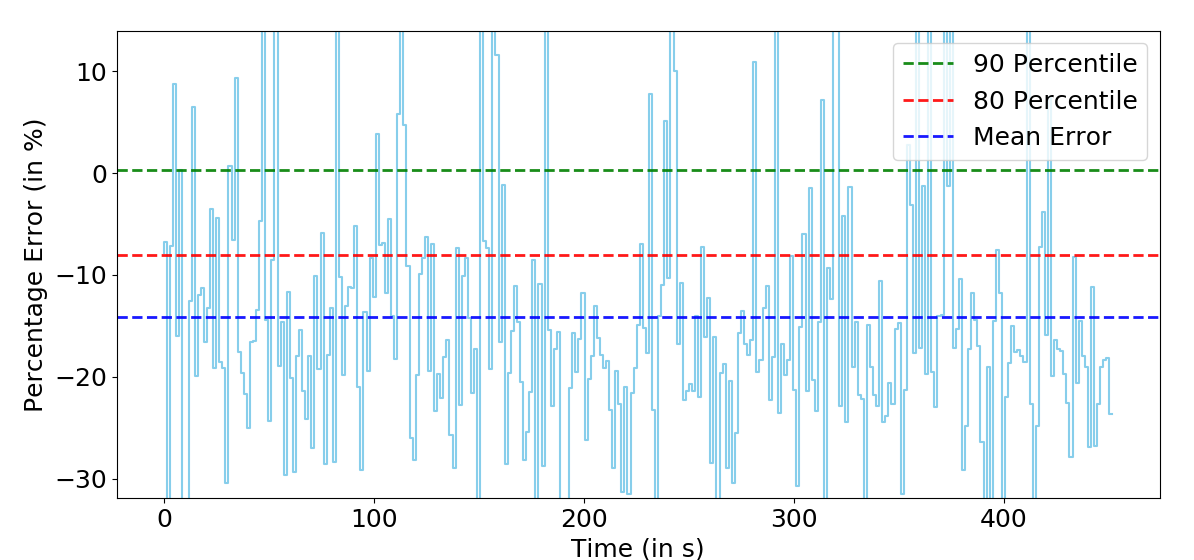
\includegraphics[width=\textwidth]{figures/sensor_error_timeline_5.png}
         \caption{Timeline on Moto Z3}
         \label{fig:sensor_error_timeline}
     \end{subfigure}
     \hfill
\fi

\begin{minipage}{0.48\columnwidth}
\begin{subfigure}[b]{\textwidth}
         \centering
         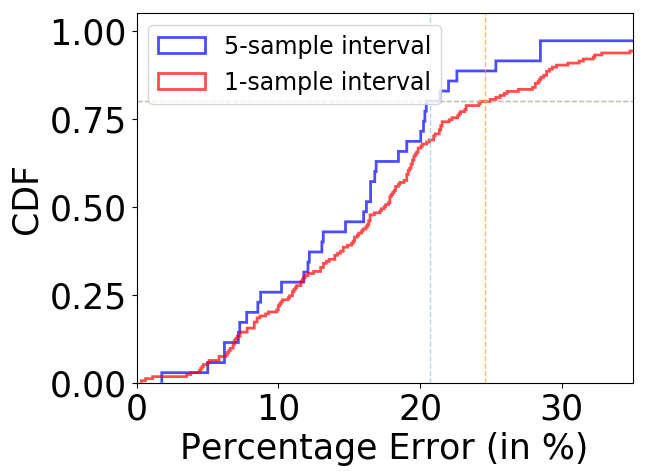
\includegraphics[width=\textwidth]{figures/sensor_error_cdf.png}
         % \caption{CDF for Moto Z3}
%         \label{fig:sensor_error_cdf_motoz3}
     \end{subfigure}
     
  \if 0
  \begin{subfigure}[b]{0.46\columnwidth}
         \centering
         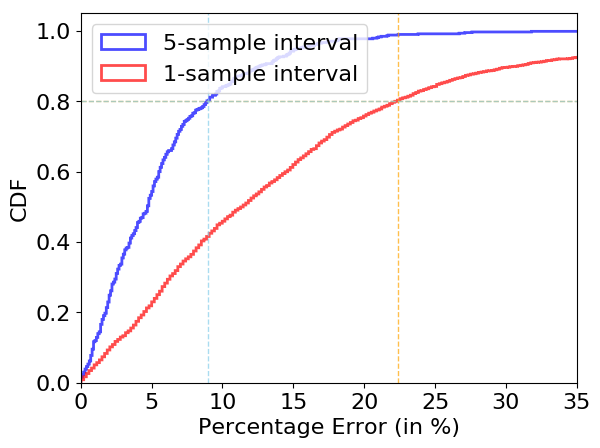
\includegraphics[width=\textwidth]{figures/sensor_error_cdf_nexus6.png}
         \caption{CDF for Nexus 6}
         \label{fig:sensor_error_cdf_nexus6}
     \end{subfigure}
  \fi
  \caption{Power sensor reading error relative to power monitor reading
        for the YouTube for Moto Z3.
        % In CDF, the orange line represents the 80 percentage for 1 sample and blue line represents for 5 sample
        }
        \label{fig:sensor_error}
        \vspace{-0.1in}
\end{minipage}
\hfill
\begin{minipage}{0.48\columnwidth}

    \centering
    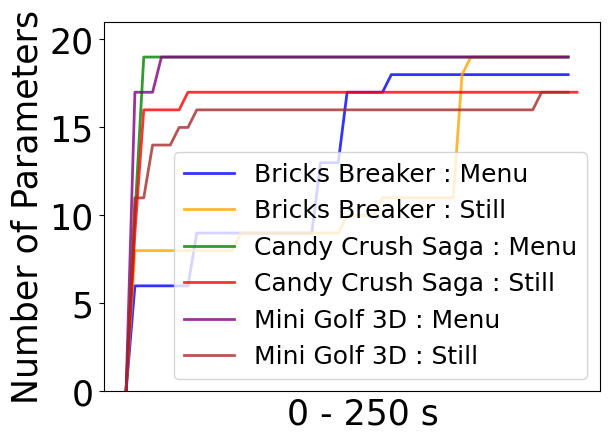
\includegraphics[width=\textwidth]{figures/004_Pixel4_cummulative_macro_parameters.png}
    \vspace{-0.1in}
    \caption{The cumulative number of unique parameters over app run duration on Pixel 4.}
    \label{fig:number_parameters_vs_duration}
    \vspace{-0.1in}
\end{minipage}
\end{figure}


 

%{\bf Findings}
%% 3. Explain power sensor is effects the accuracy of the equations
%Figure~\ref{fig:sensor_error} shows the timeline and the CDF for the sensor error.
\if 0
Figure~\ref{fig:sensor_error_timeline} shows the percentage error of the estimated energy
for 1-sample intervals (1.4s) based on power sensor reading over the 500s app run for Moto Z3.
We observe that \comment{for 89.7\% of the intervals the power sensor reading underestimates the energy drain compared to the power monitor reading.}
\fi

Figure~\ref{fig:sensor_error} shows the CDF for the absolute
percentage error on Moto Z3 for 1-sample (1.4s) and for 5-sample (7s)
intervals.  We plot the error for 5-sample intervals to see if
averaging over 5 samples can reduce the power sensor reading error.
% since if so we can set up an equation for each 5-sample interval as opposed to each 1-sample interval.
Figure~\ref{fig:sensor_error} shows
that the average error for 5-sample intervals, 15.84\%,
is only slightly better than that for 1-sample intervals, 19.01\%.
Similarly, the 80th percentile errors for 1-sample and 5-sample intervals
are 20.52\% and 24.18\% and median errors are 
16.76\% and 17.99\%, respectively.

\if 0
% , and the 80th percentile errors are 24.03\% and 21.10\%, respectively.
% Nexus 6
Figure~\ref{fig:sensor_error_cdf_nexus6} shows the CDF for the absolute percentage error
for 1-sample intervals (175 ms) and for 5-sample intervals (875 ms) for Nexus 6.
However, we see that the average error for 5-sample intervals, 7.21\%,
is lower than for 1-sample intervals of 19.06\%, and
the 80th percentile errors are 9.89\% and 26.60\%, respectively.
\comment{We observe that the sensor is about 3 times lower in Nexus 6 as compared to Moto Z3
for 1 sample interval is due to the interval of Nexus 6 being 8 times shorter than Moto Z3.
Suggesting that the low sampling rate of the sensor is the cause of the error.}
\fi
Such high error 
suggests that the built-in power sensor readings available on today's Android phones 
are not suitable for self power model derivation. 
Thus we conduct our SPMD study by using an external
Monsoon power monitor to generate the power draw ground truth.

\if 0
{\bf Reason }
%% 5. Reasons for the inaccuracies in power sensor
The high inaccuracy of the power sensor could be attributed to mainly 2 reasons.
\begin{itemize}
    \item {\bf Noise: } The power management circuit and it's location in the device is susceptible to noise due to the electronic circuitry involved in it.
    It can be argued that, the noise can be reduced by taking a longer interval which might average out the effect of noise, but from our finding we find that this approach is not effective.
    
    \item {\bf Low Sampling rate: } The power sensor generate a new value every 1.4 seconds interval in moto Z3.
    This greatly inhabits use of the power sensor to gather instantaneous current. 
 \end{itemize}
\fi


% The Monsoon power monitor has a sampling rate of 5 KHz  and has been widely used as the ground truth in smartphone power modeling and energy drain studies. 


\subsection{Aligning Power Monitor with Linux event trace}
\label{subsec:align}

As in TPMD, using an external power monitor in SPMD faces the challenge
of aligning the power monitor reading trace with the power event trace
logged on the phone, as the power monitor has a separate clock and
thus clock drifts from that of the phone. Accurate alignment is
critical to post-processing of SPMD as it directly affects how well the
two sides of each equation in the system of equations capture the same
time interval.

We achieve accurate trace alignment in two steps.  First, we run a
``beacon'' microbenchmark consisting of a 5-second CPU burst, and
align the time of the CPU utilization surge in the event trace with
the time of the corresponding square wave in the power monitor
readings. This gives us coarse-grained alignment, at the 100ms scale.

\begin{figure}[tp]
    \vspace{-0.1in}
    \centering
    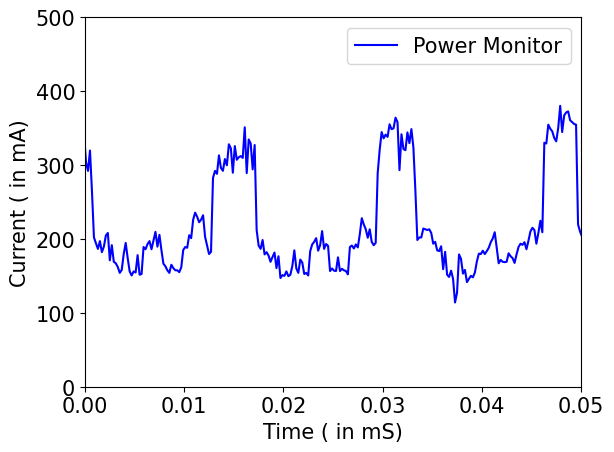
\includegraphics[width=0.50\columnwidth]{figures/candy_crush_saga_menu_timeline.png}
    \vspace{-0.1in}
    \caption{A snippet of power monitor readings for Candy Crush Saga Menu scenario on Moto Z3.}
    \label{fig:power_trace_candycrush_menu}
    \vspace{-0.2in}
\end{figure}

Second, we perform fine-grained alignment at the 1ms scale, which is
required in our feasibility study to explore SPMD at different
time scales (in \S\ref{sec:modelling_macro}--\S\ref{sec:micronano}).
The basic idea is try to match the parts of the two traces
for the same rendering interval (which has a duration of 16.7ms).
Figure~\ref{fig:power_trace_candycrush_menu} shows that
a typical rendering interval contains a GPU Busy phase followed
by a GPU Idle phase, and the Busy phase is marked
by a sharp rising edge and a sharp failing edge.
However, adjacent rendering intervals
typically have very similar power draw curves.
%  A modern smartphone on an average can generate 60 frames per second.
From the event trace we observe that the time taken to generate frames
by the GPU, \ie between two consecutive rising edges,  vary slightly, \eg
% Figure~\ref{fig:distribution_gpu_interval} shows the rendering interval spread
% for the 6 app scenarios collected from event trace.
% Our measurements shows that
the standard deviation 
for the 6 app scenarios ranges between 0.37-1.54 ms, 0.24-0.57 ms,
 and 0.10-1.42 ms,
respectively, on the 3 phones.
%   This poses a significant challenge to aligning 
%   the power monitor reading trace with the Linux event trace that we collected
%   for extracting the timings when the phone components enter different power states.
%
%   Given a power monitor trace, we mark the rising edge as the start of a
%   rendering interval and the falling edge as the end of the GPU
%   Active-busy state 
We exploit this variation in aligning the corresponding rendering intervals
in the two traces as follows.
After the coarse-grained alignment,
we choose the 50-interval window \dcomment{within 100ms offset} from the power monitor trace that has
the highest standard deviation in rendering interval durations.
%  and GPU Active-busy duration (across all of the 50 intervals).  
Next, from the event trace we use a sliding window to find the window
whose inter-GPU Busy timings best fits those of the chosen power trace window.
% 50-interval window of the power monitor trace.

% We choose a 50 interval window which we slide across 10 seconds in the middle of the trace.
% The cost function chosen is the L1-norm of the standard deviation of the total interval and
% the GPU Active-busy interval. We choose the 50 interval which has the least standard deviation.
% To align it with the event trace, we use L2 norm of the difference in the total interval
% and GPU Active-busy interval over a sliding window. 

\section{Experimental Setup}
\label{sec:etup}


%% 2. Explain the device used

% We carried our SPMD on three phones with fairly diverse hardware.
% Moto Z3 is a representative of recent phone.
% It has a Kryo Qualcomm SOC~\cite{snapdragon835} based on the big.LITTLE architecture
% with 4 LITTLE cores (22 frequencies) and 4 big cores (31 frequencies), and
% an Adreno 540 GPU which can run at 7 different frequencies.
 
% In contrast, the Nexus 6 was a representative of the generation before
% the big.LITTLE architecture, with a Krait Qualcomm SOC~\cite{snapdragon805} that
% has 4 cores which can independently operate at 18 different frequencies, and
% an Adreno 420 GPU  which can run at 5 different frequencies.

% In our experiments, we simplified the SPMD modeling task by turning off the LITTLE cores on Moto Z3
% % for all our experiments, hence all our results are based on big cores.
% which reduces the number of parameters in the modeling equations.
% As we will see below, even with this simplification, making SPMD to work is already difficult. 

% Since we focus our SPMD experiments on two phone components, the CPU and GPU,
% we used a set of {three} popular game apps which are known to predominantly
% use only the CPU and GPU. The apps have diverse GPU and CPU utilization. 
% For example, the average GPU utilization is 38.0\% for Pottery,
% 25.92\% for Candy Crush Saga and 16.0\% for Bricks Breaker on Moto Z3.

We carried our SPMD on three representative phones from three generations,
Pixel 2, MotoZ3, and Pixel 4 released in 2017, 2018, and 2019, respectively.
Pixel 2 and Moto Z3 have a Kryo Qualcomm SOC Snapdragon 835 each~\cite{snapdragon835} and Pixel
4 has a Snapdragon 855~\cite{snapdragon855}. Both SOCs are based on the
big.LITTLE architecture.  
% Pixel 2 and Moto Z3 
Snapdragon 835 has a CPU with 22 LITTLE-core and 31 big-core frequencies, 
and an Adreno 540 GPU which can run at 7 different frequencies.
Snapdragon 855 has a CPU with 18 LITTLE-core and 20 big-core frequencies,  
and an Adreno 640 GPU which can run at 5 different frequencies.

For our experiments, we simplified the SPMD modeling task by turning
off the LITTLE cores \dcomment{ and 2 big cores}
on the phones % Moto Z3
% for all our experiments, hence all our results are based on big cores.
which reduces the number of parameters in the modeling equations.
As we will see below, even with this simplification, making SPMD to work is difficult. 
Since we focus our SPMD experiments on two of the phone components, the CPU and GPU,
we use a set of {three} popular game apps, shown in Table~\ref{tab:app_scenario_description},
that are known to be predominantly
using only the CPU and GPU. We found that the apps have diverse GPU and CPU utilization. 
% For example, the average GPU utilization is 38.0\% for Mini Golf 3D,
% 25.92\% for Candy Crush Saga and 16.0\% for Bricks Breaker on Moto Z3.
% \comment{Utilisation not final yet???}
For example, the average GPU utilization is 49.57\% for Mini Golf 3D Still,
22.32\% for Candy Crush Saga Still and 12.20\% for Bricks Breaker Still on Moto Z3.
We further consider two scenarios from each of these apps,
as listed in Table~\ref{tab:app_scenario_description}.

\begin{table}[tp]
    \centering
    \caption{App scenario description.}
    \vspace{-0.1in}
    {\small
        \begin{tabular}{|p{15mm}|p{12mm}|p{46mm}|}
        \hline
        App & Scenario & Description \\
        \hline
        \hline
             \multirow{2}{15mm}{Bricks Breaker} & Menu & Menu page\\
             \cline{2-3}
             & Still & Game running without any input \\
             \hline
             \multirow{2}{15mm}{Candy Crush Saga} & Menu & Menu Page\\
             \cline{2-3}
             & Still &  Game running without any input \\
             \hline
             \multirow{2}{15mm}{Mini Golf 3D} & Menu & Menu Page \\
             \cline{2-3}
             & Still &  Game running without any input \\
            \hline
        \end{tabular}
    }
    \label{tab:app_scenario_description}
    \vspace{-0.2in}
\end{table}

We generated a 250-second run for each of the app scenarios with the
phone attached to the power monitor.  For the three phones Pixel 2,
Moto Z3 and Pixel 4, we kept the screen dark and removed its constant
power draw of 43mA, 57mA and 78mA, respectively, from the power monitor
measurement in setting up the equations.  For each scenario, we left the
app running without any user input.

% \paragraph{Aligning power trigger trace with power monitor readings}
% When readings from the Monsoon external power monitor, either as ground truth in model accuracy calculation or as the left-hand-side (LHS) value of the modeling equations, 


% The results we observed from our experiment can be easily extended by including corresponding triggers for the case while all the cores are running .

% Finally, we found that the findings for the three phones are  very similar.
% We thus moved all the results for Nexus 6 
% to~\cite{longversion} due to page limit.


% \section{Per-Component SPMD on Modern Phones}
% \label{sec:evaluation}

% In this section, we present the experience with trying to make SPMD work
% on two modern phones. We show even when focusing on only two phone components, CPU and GPU, 
% applying SPMD faces a number of fundamental challenges. 



\section{Component-wise SPMD at Macro Scale}
\label{sec:modelling_macro}

We first explore {\em SPMD at macro-scale}, \ie setting one equation
for each interval at the second-scale, \eg between 1 to 5 seconds,
based on two justifications.  First, the power monitor reading
resolution of 0.2ms allows us to have accurate energy (average power
draw) readings at the 1-second granularity. Second, since the GPU
typically goes through the Busy and Idle states at least once in every
16.7ms, using intervals at the second-scale potentially allows us to capture 
diverse GPU and CPU usage, \eg over 
60 or more such rendering intervals, which helps
the regression solver to output meaningful solutions.


\begin{figure*}[tb]
    \centering
    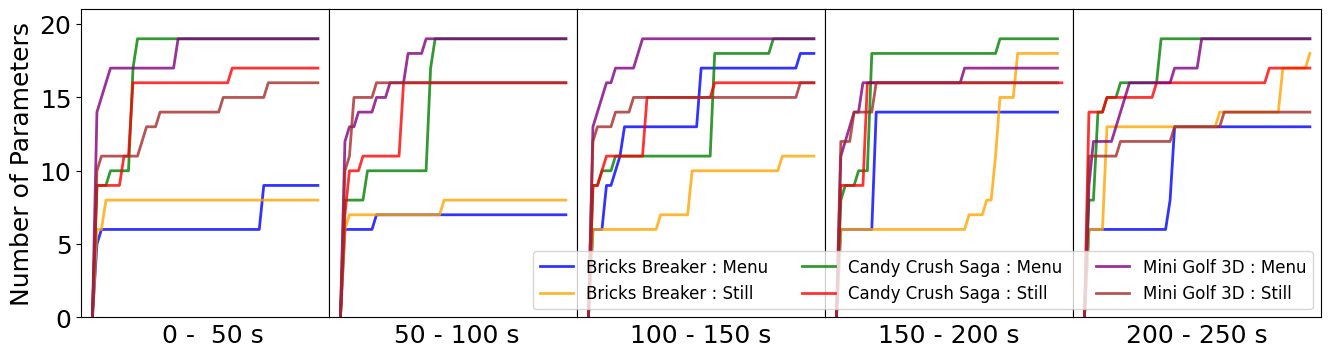
\includegraphics[width=\textwidth]{figures/004_Pixel4_cummulative_parameters.png}
    \vspace{-0.2in}
    \caption{The cumulative number of unique parameters over app run duration in five 50-second segments on Pixel 4.}
    \label{fig:number_parameters_vs_duration_100s}
    \vspace{-0.1in}
\end{figure*}

\paragraph{How Many Systems of Equations?}
\label{subsec:relation}
Since our app run duration are of 250 seconds each, under macro-scale
SPMD, varying per-equation time interval $t_e$ between 1s to 5s gives us
between 50 to 250 equations. To explore how many equations should be
used, we first measure how the number of unique model parameters
varies with the app run duration.

Figure~\ref{fig:number_parameters_vs_duration} shows the cumulative
number of unique power model parameters over a 250-second app run
duration for the six app scenarios on Pixel 4. We make the following
observations.
(1) The number of unique model parameters increases with the app run
duration, with the maximum ranging between 17 (for the Candy Crush Saga Still
scenario) and 19 for (the Mini Golf 3D Menu scenario).
(2) The GPU stayed at one frequency and contributed 2 parameters (Busy
and Idle power in that frequency) for all 6 app scenarios, and the
remaining 15 to 17 parameters are CPU core model parameters.  Similar
trends are observed for the other two phones.

Figure~\ref{fig:number_parameters_vs_duration} does not show the
number of unique model parameters in smaller segments of the app
run.  To see this, we plot in
Figure~\ref{fig:number_parameters_vs_duration_100s} the cumulative
number of unique model parameters over each 50-second time
segment, for the 6 app scenarios.  We see that the curves for all 
five 50-second segments look very similar, suggesting that the apps'
usage of both the CPU and GPU are similar.  However, the total number
of unique model parameters in each of the 50-second segment is
lower when compared with the full 250-second segment. For example, 
with Bricks Breaker Menu, the number of parameters is 18
for the 250-second segment but
reduces to 9, 7, 18, 14 and 13
for the 5 smaller segments.
This suggests that creating a system of equations for a shorter epoch in general may have
fewer unknowns than for a longer epoch.
% \dcomment{'Clarify epoch'}

\if 0
\cut{ 
\begin{figure}[tp]
    \centering
    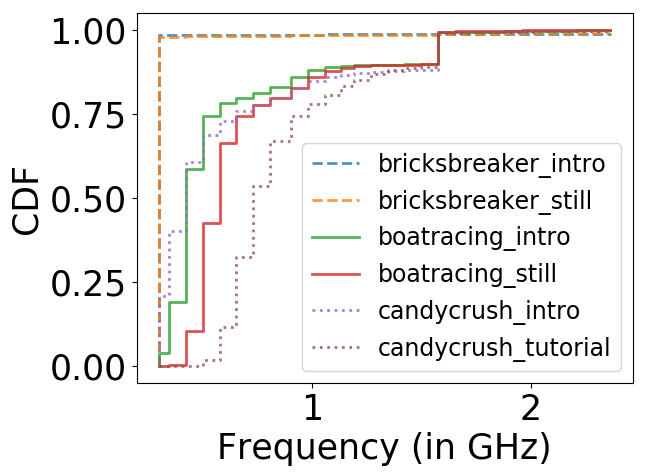
\includegraphics[width=0.65\columnwidth]{figures/cdf_frequency_residence.png}
    \vspace{-0.1in}
    \caption{CDF of the total time spent in each CPU frequencies for 6 app scenarios.}
    \label{fig:cdf_frequency_residence}
    \vspace{-0.1in}
\end{figure}

Finally, to understand how the utilization of different model
parameters vary, we plot in Figure~\ref{fig:cdf_frequency_residence}
the CDF of the percentage of the total time (250 seconds) spent in
each CPU core frequency for the six scenarios. We see the utilizations
are uneven: the top 5 parameters in each app scenario account for
75.20\% to 98.76\% of the total app run duration across the 6 app
scenarios.  In contrast, the utilization of the single GPU frequency
experience in each app scenario varies between 14.72\% and 64.51\%.  
}
\fi



Based on the above exploration, we experimented with 3 alternatives
for creating the system of equations for each app scenario, by varying
the app run duration per system between 50 and 250 seconds, and the
interval per equation between 1 and 5 seconds, while ensuring that
the number of equations per system is 50 or more. 
The 3 configurations have 50 equations of 1 second each,
250 equations of 1 second each, and 50 equation of 5 second each, respectively,
and are denoted as 50x1, 250x1, and 50x5 thereafter.

\begin{table*}[tb]
     \centering
     \begin{subfigure}[b]{0.30\textwidth}
        \centering
        \caption{50 equations with 1 second equation interval}
    	{ \scriptsize
    	\begin{tabular}{ | p{1.8cm} | p{.2cm} | p{.2cm} | p{.2cm} | p{.2cm} | p{.2cm} | p{.2cm} | }
%    	\begin{tabular}{ | l | c | c | c | c | c | c | }
    		\hline
    		     & \multicolumn{6}{ c|}{Error for each App Sc. (\%)}\\
    		\cline{2-7}
                    Model & \rot{B. Menu} & \rot{B. Still} & \rot{C. Menu} & \rot{C. Still} & \rot{M. Menu} & \rot{M. Still}  \\
    		\hline
                Unconst.             & 0.7 & 0.9 & 0.8 & 1.1 & 1.0 & 0.9 \\
                Const.               & 1.2 & 1.1 & 1.2 & 1.6 & 1.4 & 1.3 \\
                Freq. Const.         & 1.2 & 1.1 & 1.6 & 2.1 & 1.9 & 1.8 \\
                Fix. F. Const.       & 1.2 & 1.1 & 1.6 & 2.1 & 1.9 & 1.8 \\
                TPMD                 & 37 & 45 & 17 & 24 & 27 & 9.2 \\
    		\hline
    	\end{tabular}
    	}
    \end{subfigure}
    \hfill
    \begin{subfigure}[b]{0.30\textwidth}
        \centering
        \caption{250 equations with 1 second equation interval}
    	{ \scriptsize
%    	\begin{tabular}{ | p{1.3cm} | p{.2cm} | p{.2cm} | p{.2cm} | p{.2cm} | p{.2cm} | p{.2cm} | }
        \begin{tabular}{ | p{1.8cm} | p{.2cm} | p{.2cm} | p{.2cm} | p{.2cm} | p{.2cm} | p{.2cm} | }
%    	\begin{tabular}{ | l | c | c | c | c | c | c | }
    		\hline
    		     & \multicolumn{6}{ c|}{Error for each App Sc. (\%)}\\
    		\cline{2-7}
                    Model & \rot{B. Menu} & \rot{B. Still} & \rot{C. Menu} & \rot{C. Still} & \rot{M. Menu} & \rot{M. Still}  \\
    		\hline
                Unconst.             & 0.8 & 0.7 & 1.4 & 1.4 & 1.1 & 1.2 \\
                Const.               & 1.0 & 0.8 & 1.3 & 1.5 & 1.2 & 1.3 \\
                Freq. Const.         & 1.0 & 0.9 & 1.4 & 1.8 & 1.3 & 1.4 \\
                Fix. F. Const.       & 1.0 & 0.9 & 1.4 & 1.8 & 1.3 & 1.4 \\
                TPMD                 & 37 & 45 & 17 & 24 & 27 & 8.5 \\
    		\hline
    	\end{tabular}
    	}
    \end{subfigure}
    \hfill
    \begin{subfigure}[b]{0.30\textwidth}
        \centering
        \caption{50 equations with 5 second equation interval}
    	{ \scriptsize
%    	\begin{tabular}{ | p{1.30cm} | p{.2cm} | p{.2cm} | p{.2cm} | p{.2cm} | p{.2cm} | p{.2cm} | }
        \begin{tabular}{ | p{1.8cm} | p{.2cm} | p{.2cm} | p{.2cm} | p{.2cm} | p{.2cm} | p{.2cm} | }
%    	\begin{tabular}{ | l | c | c | c | c | c | c | }
    		\hline
    		     & \multicolumn{6}{ c|}{Error for each App Sc. (\%)}\\
    		\cline{2-7}
                    Model & \rot{B. Menu} & \rot{B. Still} & \rot{C. Menu} & \rot{C. Still} & \rot{M. Menu} & \rot{M. Still}  \\
    		\hline
                Unconst.             & 0.4 & 0.4 & 0.7 & 0.7 & 0.5 & 0.6 \\
                Const.               & 0.6 & 0.4 & 0.8 & 0.9 & 0.6 & 0.8 \\
                Freq. Const.         & 0.7 & 0.5 & 1.0 & 1.2 & 0.9 & 1.1 \\
                Fix. F. Const.       & 0.7 & 0.5 & 1.0 & 1.2 & 0.9 & 1.1 \\
                TPMD                 & 37 & 45 & 17 & 24 & 27 & 8.5 \\
    		\hline
    	\end{tabular}
    	}
    \end{subfigure}
    \caption{Showing error for all app scenarios for 3 ways of creating the system of equations.}
    \label{tab:macro_3_ways_error}
    \vspace{-0.1in}
\end{table*}

\begin{figure*}[tb]
    \centering
    \begin{subfigure}[b]{0.75\textwidth}
         \centering
         
\includegraphics[width=\textwidth]{figures/label_equations.png}
    \end{subfigure}
    \\
    \hfill
    \centering
     \begin{subfigure}[b]{0.32\textwidth}
         \centering
         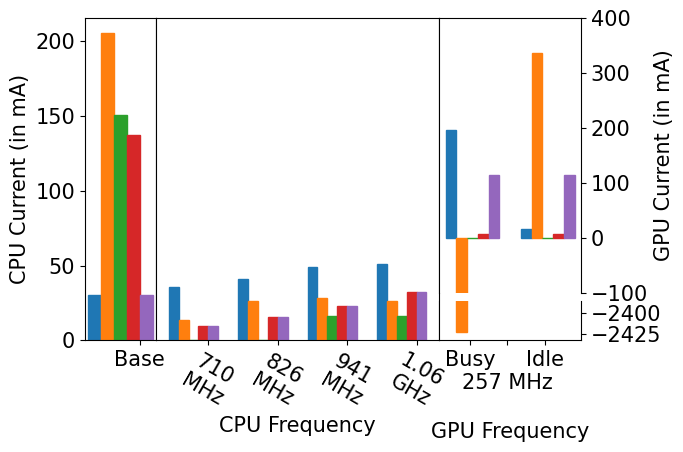
\includegraphics[width=\textwidth]{figures/004_Pixel4_bricksbreaker_menu_50_1_equations.png}
         \caption{50 equations with 1 second equation interval}
         \label{fig:macro_3_ways_50_1}
     \end{subfigure}
    \begin{subfigure}[b]{0.32\textwidth}
         \centering
         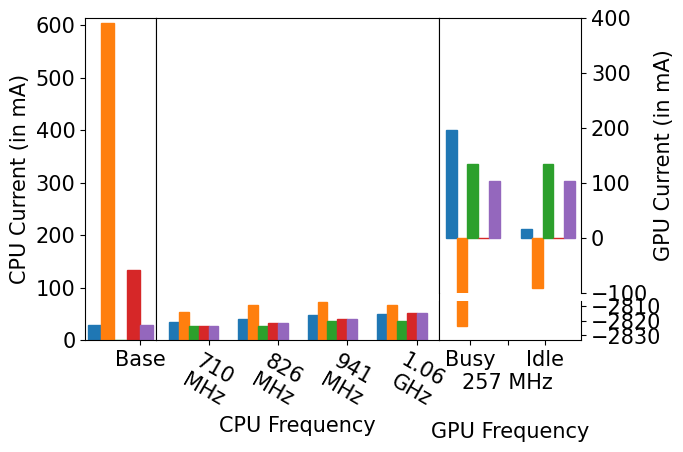
\includegraphics[width=\textwidth]{figures/004_Pixel4_bricksbreaker_menu_250_1_equations.png}
         \caption{250 equations with 1 seconds equation interval}
         \label{fig:macro_3_ways_250_1}
     \end{subfigure}
    \begin{subfigure}[b]{0.32\textwidth}
         \centering
         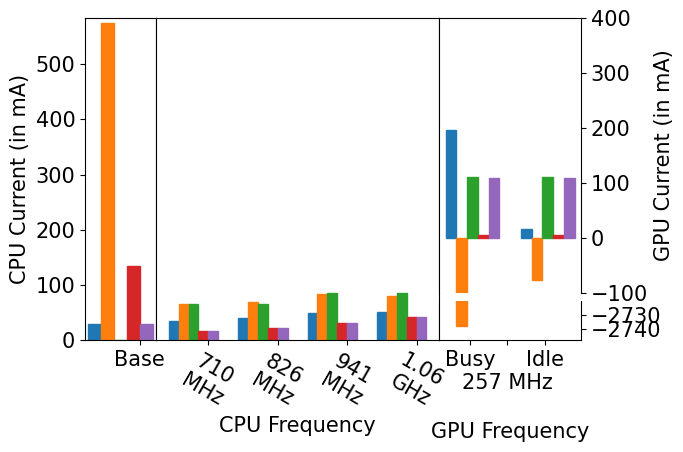
\includegraphics[width=\textwidth]{figures/004_Pixel4_bricksbreaker_menu_250_5_equations.png}
         \caption{50 equations with 5 seconds equation interval}
         \label{fig:macro_3_ways_50_5}
     \end{subfigure}
         \caption{SPMD models for Bricks Breaker Menu scenario on Pixel 4 under
         3 ways of creating the system of equations. 
         (Only model parameters for 4 CPU frequencies with highest utilization are shown due to space constraint.).}
    \label{fig:macro_3_ways}
    \vspace{-0.1in}
\end{figure*}

\paragraph{Detail results on Pixel 4.}
Table~\ref{tab:macro_3_ways_error} summarizes the \comment{mean
  prediction error per equation} of the SPMD models using different
versions of the regression solver for the six app scenarios under the
three ways of creating systems of equations, \comment{on Pixel 4.}
%  \comment{The findings for the other app scenarios and on the other two phones            
% are similar and are omitted due to page limit.}.                                          
We observe that (1) The prediction error only increases slightly as
more constraints are imposed on the regression solver,
\eg from 0.7\%--1.1\% for the unconstrained solver to  1.1\% --1.8\% for
the Fix. Freq. Const version of the solver, for the 50x1 system.
(2) The prediction of SPMD model under the most constrained regression solver,
Fix. Freq. Const, is far lower than that for the TPMD model, \eg ranging
between 9.2\%--45\% for the 50x1 sytem.
(3) The prediction error are consistently low and similar across the
three ways of creating systems of equations, ranging between
1.1\%--1.8\%, 0.9\%--1.8\%, and 0.5\%--1.2\% under the Fix. Freq. Const solver
for the 50x1, 250x1, and 50x5 systems, respectively.

We next look into the actual power model parameters generated by SPMD
for one app scenario in detail.
Figure~\ref{fig:macro_3_ways} shows
the solutions found with these 3 alternative ways of creating systems of
equations for Bricks Breaker Menu scenario on Pixel 4.
For comparison, we include the model parameters derived from
TPMD. We note
that although in general TPMD models are app-agnostic, we listed the
GPU parameters derived for the corresponding app scenarios (as shown
in Figure 1) as the TPMD models here to show how close SPMD-derived
models match the ``carefully'' generated TPMD-derived model.

\st{First, we observed that the ranks of the system of equations is less
than the number of model parameters by more than 1.  The reason is
that the base power shows up in all equations which does not
contribute to the rank.}

\st{As expected, since the systems are under-ranked, the model parameters
output from the unconstrained regression solver look very different
from those found from the TPMD model.}
For the {\it unconstrained solver},
the parameters generated, shown in Figure~\ref{fig:macro_3_ways},
violate some basic properties:
(1) some model parameters generated are negative, \eg the GPU Busy
component power is -2422.15 mA for the 50x1 system  and
is -2737.61 mA for the 50x5 system; and 
%  (2) the CPU power draw at a lower frequency may be higher than the
%  power draw at a higher frequency (for all 3 systems);
(2) The base CPU power for 50x1, 250x1 and 50x5 systems 
is 6.8$\times$, 20.0$\times$, and 19.4$\times$ higher 
than its counterpart in the TPMD model, respectively.
% (3) the GPU Idle power draw generated is higher than the GPU Busy
% power (for all 3 systems). \comment{I do not see that???}

For the {\it constrained solver}, while the parameters generated,
shown as "Constrained" in Figure~\ref{fig:macro_3_ways}, are all
positive and non-decreasing with increasing frequencies, the
CPU power parameters still do not satisfy the monotonicity property;
the parameters for consecutive frequencies often stay the same. 
For example, 
% for the Bricks Breaker Menu scenario,
the CPU power stays at
65.78 mA for 2 of the frequencies from 710 MHz and 825 MHz and again
remains at 86.39 mA for 8 of the frequencies from 941 MHz to 1.80 GHz
for the 50x5 system.

For the {\em Frequency-constrained} solver, the parameters generated, shown in
in Figure~\ref{fig:macro_3_ways}, look very much similar to those in
the TPMD model, but the base power draw ranges between 133.08 mA to
137.11 mA, which is over 4.4$\times$ higher than their counterpart of
30.12 mA observed in the TPMD model for the 3 systems.

{\color{blue}To summarize, by carefully examining the SPMD learning results, we find that }(1) The model parameters differ significantly from
TPMD. For example, for Brick Breakers 50x5 systems, CPU parameters at CPU frequency of
1.61 GHz and 1.92GHz is 133.9 mA and 221.9 mA instead of 85.70 mA and 128.0 mA instead of
TPMD parameters. Also, the power parameters range between
0.28$\times$-1.07$\times$,
0.79$\times$-1.81$\times$,
0.48$\times$-1.86$\times$ their
TPMD counterparts for CPU frequency for the 3 systems.
 %
(2) The GPU Busy and GPU Idle power parameters have the same value in "Fix. F. Const."{\color{blue}--!!!---change this part (tables, figures, values) if you remove Fix. F. Const.---!!!---}
but the counterparts in the TPMD model, the Busy power states is more than 15$\times$
larger than Idle power state.
For example, both parameters are 0.0 mA, 99.1 mA amd 109.2 mA for Bricks Breaker Menu
on all the 3 phones respectively.

\st{To overcome the under-rank problem, we fixed the base power to the
constant value of 30.12 mA as seen in the TPMD model which makes the
rank equal to the number of parameters for the 3 systems. 
With this approach, the parameters generated by the solver, 
shown in the rows labeled "Fix. F. Const.",
only changed slightly;}{\color{blue}---!!!--because we don't need rank, maybe we can remove the Fix. F. Const in the table?--!!!-} 
% the solver split the excessive base power and
% moved them into the GPU Busy and Idle power, and as a result the trend of all the
% parameters now look similar to those observed in the TPMD model.
% \comment{
% However, the generated model parameters still suffer two major problems: 
% (1) The model parameters differ significantly from
% TPMD. For example, for Brick Breakers 50x5 systems, CPU parameters at CPU frequency of
% 1.61 GHz and 1.92GHz is 133.9 mA and 221.9 mA instead of 85.70 mA and 128.0 mA instead of
% TPMD parameters.
% % Similarly, we observe for GPU parameters, Busy and Idle power parameters are both
% % 109.2 mA instead of 196.6 mA and 15.81 mA TPMD parameters.
% Also, the power parameters range between
% 0.28$\times$-1.07$\times$,
% 0.79$\times$-1.81$\times$,
% 0.48$\times$-1.86$\times$ their
% TPMD counterparts for CPU frequency for the 3 systems.
%  %
% (2) The GPU Busy and GPU Idle power parameters have the same value in "Fix. F. Const."{\color{cyan}--!!!---change this part if you remove Fix. F. Const.---!!!---}
% but the counterparts in the TPMD model, the Busy power states is more than 15$\times$
% larger than Idle power state.
% For example, both parameters are 0.0 mA, 99.1 mA amd 109.2 mA for Bricks Breaker Menu
% on all the 3 phones respectively.
% }

{\color{blue}Besides those qualitative evidences that the modeling results of SPMD may be invalid, we also use F-test and $R^2$-measurement to explain the regression solutions for the SPMD modeling results are not valid. --!!-PLEASE FILL RESULTS HERE-!!--}
\dcomment{
We observe that the $R^2$ value varies between 0.05-0.97, 0.24-0.97 and 0.47-0.89 for the
three phones respectively. This shows that for some app scenarios the
curve\_fit fail.
For example, for Candy Crush Still in Pixel 4 the $R^2$ is 0.47.
The inability of able to fit is showed in the average error of
1.2\% which is the highest among of all the app scenarios in Pixel 4.
The minimum singular value is 4.6e-4,
causing the system susceptibility to
$4.6e-4^{-1}$$\approx$$2173\times$ the measurement noise.
% The min singular values fall in the 
The the minimum singular values are between
6.25e-16 - 2.20e-3,
9.65e-19 - 6.12e-3
and
4.58e-20 - 3.67e-3 for the 3 phones respectively.
% The min and max singular values differs by 5.21e+3$\times$-1.01e+6$\times$,
% 2.16e+3$\times$-1.35e+16$\times$ and 1.75e+3$\times$-1.02e+20$\times$ for the 3 phones.
% The large ratio means that the system of equations are very sensitive to any noise.
}

% \paragraph{Results and Validation.}
% Using the 50x5 system of equations, we applied the
% Fix. F. Const. {\color{cyan}!!!--Again, need change if remove Fix. F. Const--!!!} version of SPMD to all 6 app
% scenarios. Figures~\ref{fig:macro_equations}(a)-(c)
% show that SPMD generated models result in much smaller 
% predictor erros for all 6 app scenarios compared to the TPMD generated models.
% However, Figures~\ref{fig:macro_equations}(d)-(f)
% again show that the SPMD-generated model
% parameter suffer the same two problems
% as in the case of the Bricks Breaker Menu scenario, \ie 
% \comment{(1) The model parameters differ significantly from
%   TPMD; (2) The GPU Busy and GPU Idle power parameters are similar
%   which are very different from their counterparts in the TPMD model.}

\begin{figure*}[tb]
     \centering
     \begin{subfigure}[b]{0.32\textwidth}
        \centering
	    \caption{Pixel 2: TPMD vs macro-SPMD error}
	    \vspace{-0.05in}
    	{ \scriptsize
%    	\begin{tabular}{ | p{1.3cm} | p{.2cm} | p{.2cm} | p{.2cm} | p{.2cm} | p{.2cm} | p{.2cm} | }
        \begin{tabular}{ | p{1.8cm} | p{.2cm} | p{.2cm} | p{.2cm} | p{.2cm} | p{.2cm} | p{.2cm} | }
%    	\begin{tabular}{ | l | c | c | c | c | c | c | }
    		\hline
    		     & \multicolumn{6}{ c|}{Error for each App Sc. (\%)}\\
    		\cline{2-7}
                    Model & \rot{B. Menu} & \rot{B. Still} & \rot{C. Menu} & \rot{C. Still} & \rot{M. Menu} & \rot{M. Still}  \\
    		\hline
                Fix. F. Const.       & 0.9 & 1.1 & 1.2 & 0.6 & 0.8 & 0.7 \\
                TPMD                 & 18 & 28 & 13 & 3.4 & 45 & 6.0 \\
    		\hline
    	\end{tabular}
    	}
    	% \vspace{-0.05in}
	    % \caption{Pixel 2: TPMD vs macro-SPMD error}
    \end{subfigure}
    \hfill
    \begin{subfigure}[b]{0.32\textwidth}
        \centering
        \vspace{-0.3in}
	    \caption{Moto Z3: TPMD vs macro-SPMD error}
	    \vspace{-0.05in}
    	{ \scriptsize
%    	\begin{tabular}{ | p{1.3cm} | p{.2cm} | p{.2cm} | p{.2cm} | p{.2cm} | p{.2cm} | p{.2cm} | }
        \begin{tabular}{ | p{1.8cm} | p{.2cm} | p{.2cm} | p{.2cm} | p{.2cm} | p{.2cm} | p{.2cm} | }
%    	\begin{tabular}{ | l | c | c | c | c | c | c | }
    		\hline
    		     & \multicolumn{6}{ c|}{Error for each App Sc. (\%)}\\
    		\cline{2-7}
                    Model & \rot{B. Menu} & \rot{B. Still} & \rot{C. Menu} & \rot{C. Still} & \rot{M. Menu} & \rot{M. Still}  \\
    		\hline
                Fix. F. Const.       & 1.8 & 0.3 & 2.6 & 0.4 & 0.2 & 26 \\
                TPMD                 & 39 & 11 & 31 & 19 & 5.9 & 39 \\
    		\hline
    	\end{tabular}
    	}
    	% \vspace{-0.05in}
	    % \caption{Moto Z3: TPMD vs macro-SPMD error}
    \end{subfigure}
    \hfill
    \begin{subfigure}[b]{0.32\textwidth}
        \centering
	    \caption{Pixel 4: TPMD vs macro-SPMD error}
	    \vspace{-0.05in}
    	{ \scriptsize
%    	\begin{tabular}{ | p{1.3cm} | p{.2cm} | p{.2cm} | p{.2cm} | p{.2cm} | p{.2cm} | p{.2cm} | }
        \begin{tabular}{ | p{1.8cm} | p{.2cm} | p{.2cm} | p{.2cm} | p{.2cm} | p{.2cm} | p{.2cm} | }
%    	\begin{tabular}{ | l | c | c | c | c | c | c | }
    		\hline
    		     & \multicolumn{6}{ c|}{Error for each App Sc. (\%)}\\
    		\cline{2-7}
                    Model & \rot{B. Menu} & \rot{B. Still} & \rot{C. Menu} & \rot{C. Still} & \rot{M. Menu} & \rot{M. Still}  \\
    		\hline
                Fix. F. Const.       & 0.7 & 0.5 & 1.0 & 1.2 & 0.9 & 1.1 \\
                TPMD                 & 37 & 45 & 17 & 24 & 27 & 8.5 \\
    		\hline
    	\end{tabular}
    	}
    	% \vspace{-0.05in}
	    % \caption{Pixel 4: TPMD vs macro-SPMD error}
    \end{subfigure}
    \\
         \vspace{+0.1in}
         \centering
     \begin{subfigure}[b]{\textwidth}
         \centering
         
\includegraphics[width=\textwidth]{figures/label_macro_equations.png}
    \end{subfigure}
    \\
    \hfill
    \centering
     \begin{subfigure}[b]{0.32\textwidth}
         \centering
         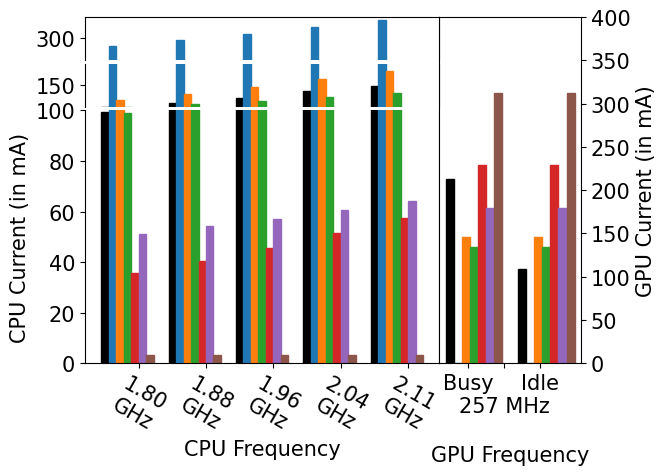
\includegraphics[width=\textwidth]{figures/002_Pixel2_250_5_macro_equations.png}
         \label{fig:macro_equations_p2}
         \vspace{-0.25in}
         \caption{Pixel 2: TPMD vs macro-SPMD coefficients}
     \end{subfigure}
    \begin{subfigure}[b]{0.32\textwidth}
         \centering
         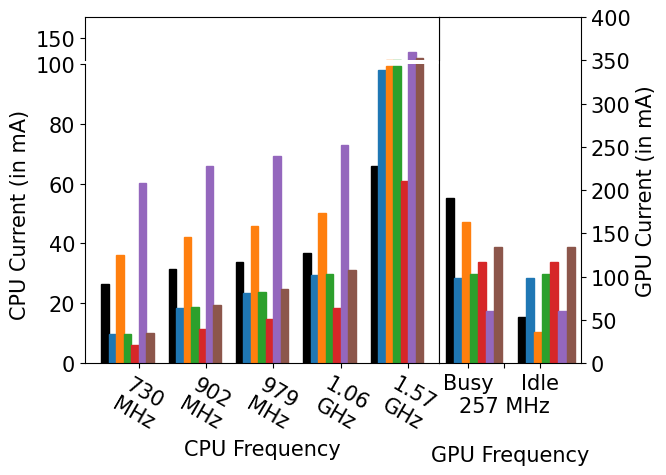
\includegraphics[width=\textwidth]{figures/003_MotoZ3_250_5_macro_equations.png}
         \label{fig:macro_equations_z3}
         \vspace{-0.25in}
         \caption{Moto Z3: TPMD vs macro-SPMD coefficients}
     \end{subfigure}
    \begin{subfigure}[b]{0.32\textwidth}
         \centering
         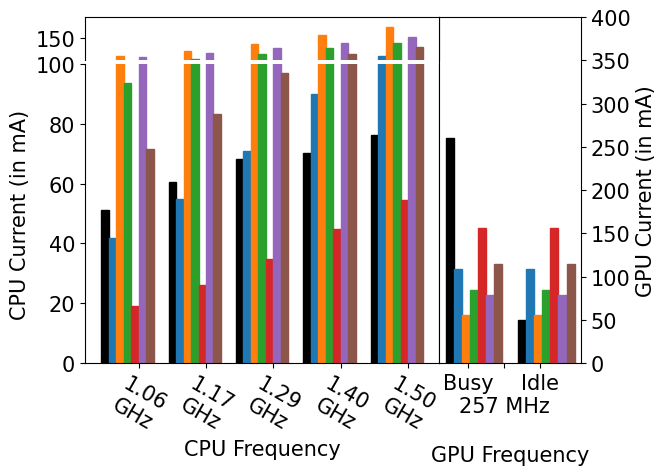
\includegraphics[width=\textwidth]{figures/004_Pixel4_250_5_macro_equations.png}
         \label{fig:macro_equations_p4}
         \vspace{-0.25in}
         \caption{Pixel 4: TPMD vs macro-SPMD coefficients}
     \end{subfigure}

    \caption{Model parameters derived by macro-scale SPMD for 50x5 system on the
        3 phones. TPMD for GPU are from Figure~\ref{fig:gpu_model}.
        (Only model parameters for 5 CPU frequencies with highest utilization are
        shown due to space constraint.) (The GPU parameter for TPMD
        is represented by average over all app scenarios GPU parameters.)}
    \label{fig:macro_equations}
   % \vspace{-0.1in}
\end{figure*}

\paragraph{Analysis.}
{\color{blue}We dig deeper into one the those experiments to \ie 50x5, to
understand why SPMD solutions are invalid. As shown in Table~\ref{tab:macro_rank_singular}, we find that the smallest singular value of the design matrix of the linear regression is close to zero. As we stated in the footnote of Page~3, this implies that the linear regression result will be very sensitive to even a small amount of noise. Roughly speaking, when equations are similar to each other, the smallest singular value of the design matrix is usually close to zero. }

% We dig deeper into one of the the full-rank system, \ie 50x5, to
% understand why SPMD generates very different parameters compared to
% TPMD.
% Since the rank of the system is already
%   full, we calculated the singular values for these equations.
%   Table~\ref{tab:macro_rank_singular} shows that each of the system
%   of equations has only 1 dominating singular value, suggesting that
%   the matrix (formed by coefficients of unknown variables in the
%   tight-hand-side (RHD) of those equations) has only one dominating
%   direction. This indicates that all the equations are basically
%   describing the same state of power usage, and thus lacks diversity.


% \begin{table*}[tb]
% \centering
% {\small
%     \caption{The rank and singular values for the set of equations for macro-scale "F. Freq. Const. SPMD" for 50x5 system on Pixel 4. (Top 11 singular values are shown.)\comment{Will reduce number of singular values later.}}
%     \vspace{-0.1in}
%     \begin{tabular}{|c|c|c|c|c|c|c|c|c|c|c|c|c|c|c|c|c|}
%     \hline
%         App & Scenario & \# of Eqns. & \# of Vars. &  \multicolumn{11}{c|}{Singular Values} & $R^{2}$ & F-Test \\
%         \hline
%          \multirow{2}{15mm}{Bricks Breaker} & Menu & 50 & 18 & 6.54  & 0.37  & 0.17  & 0.10  & 0.04  & 0.02  & 0.02  & 0.01  & 0.01  & 0.00  & 0.00 & 0.68 & \\
%          \cline{2-17}
%          & Still &  50 & 19 & 6.73  & 0.38  & 0.34  & 0.16  & 0.03  & 0.02  & 0.02  & 0.01  & 0.01  & 0.01  & 0.00 & 0.83 & \\
%          \hline
%         \multirow{2}{15mm}{Candy Crush Saga} & Menu &  50 & 19 & 6.79  & 0.49  & 0.19  & 0.10  & 0.08  & 0.03  & 0.03  & 0.02  & 0.02  & 0.01  & 0.01 & 0.73 & \\
%          \cline{2-17}
%          & Still & 50 & 17 & 6.81  & 0.52  & 0.21  & 0.10  & 0.05  & 0.05  & 0.03  & 0.02  & 0.01  & 0.01  & 0.01 & 0.47 & \\
%          \hline
%         \multirow{2}{15mm}{Mini Golf 3D} & Menu & 50 & 19 & 6.41  & 1.62  & 0.47  & 0.38  & 0.18  & 0.06  & 0.03  & 0.02  & 0.02  & 0.01  & 0.01 & 0.80 & \\
%         \cline{2-17}
% 	     & Still & 50 & 17 & 6.46  & 0.99  & 0.34  & 0.19  & 0.11  & 0.06  & 0.04  & 0.03  & 0.02  & 0.01  & 0.01 & 0.89 & \\
% 	     \hline
%     \end{tabular}
%     \label{tab:macro_rank_singular}
%     \vspace{-0.1in}
% }
% \end{table*}
\begin{table*}[tb]
\centering
{\small
    \caption{The {\color{blue}smallest }singular values for the \st{set of equations}{\color{blue}design matrix} for macro-scale "F. Freq. Const. SPMD" for 50x5 system on Pixel 4. (Smallest 11 singular values are shown.)\comment{Will reduce number of singular values later.}}
    \vspace{-0.1in}
    \begin{tabular}{|c|c|c|c|c|c|c|c|c|c|c|c|c|c|c|c|c|}
    \hline
        App & Scenario & \# of Eqns. & \# of Vars. &  \multicolumn{11}{c|}{Smallest  Singular Values} & $R^{2}$ \\
        \hline
         \multirow{2}{15mm}{Bricks Breaker} & Menu & 50 & 18 & 0.01  & 0.01  & 0.00  & 0.00  & 0.00  & 0.00  & 0.00  & 0.00  & 0.00  & 0.00  & 0.00 & 0.68 \\
         \cline{2-16}
         & Still &  50 & 19 & 0.01  & 0.01  & 0.00  & 0.00  & 0.00  & 0.00  & 0.00  & 0.00  & 0.00  & 0.00  & 0.00 & 0.83 \\
         \hline
        \multirow{2}{15mm}{Candy Crush Saga} & Menu &  50 & 19  & 0.02  & 0.01  & 0.01  & 0.01  & 0.01  & 0.01  & 0.00  & 0.00  & 0.00  & 0.00  & 0.00 & 0.73 \\
         \cline{2-16}
         & Still & 50 & 17  & 0.03  & 0.02  & 0.01  & 0.01  & 0.01  & 0.01  & 0.01  & 0.01  & 0.01  & 0.00  & 0.00 & 0.47 \\
         \hline
        \multirow{2}{15mm}{Mini Golf 3D} & Menu & 50 & 19  & 0.02  & 0.01  & 0.01  & 0.01  & 0.01  & 0.01  & 0.01  & 0.01  & 0.00  & 0.00  & 0.00 & 0.80 \\
        \cline{2-16}
	     & Still & 50 & 17  & 0.03  & 0.02  & 0.02  & 0.01  & 0.01  & 0.01  & 0.00  & 0.00  & 0.00  & 0.00  & 0.00 & 0.89 \\
	     \hline
    \end{tabular}
    \label{tab:macro_rank_singular}
    \vspace{-0.1in}
}
\end{table*}
% In addition to lack of diversity in phone component usage which contributed 
% to the sparse singular values, we found that the energy values in LHS of
% the equation   appear to contain  measurement noise which further prevents
% the regression solver from generating meaningful solutions. To see this,
% we plot the distribution of the LHS energy values of the  equations in the
% two systems 250x1 and 50x5, Figures~\ref{fig:y_distribution}(a)-(b) show the
% energy values for the two systems are clustered in a Gaussian distribution
% with standard deviation of 3.04 mA and 5.72 mA, each of which is less than
% 2.45\% compared with the mean value. This Gaussian-like distribution suggests
% that the LHS values of the equations contain measurement noise.
% \comment{PZ: this is not obvious????}

% \begin{figure}[tb]
%     \vspace{-0.1in}
%     \centering
%          \begin{subfigure}[b]{0.49\columnwidth}
%          \centering
%          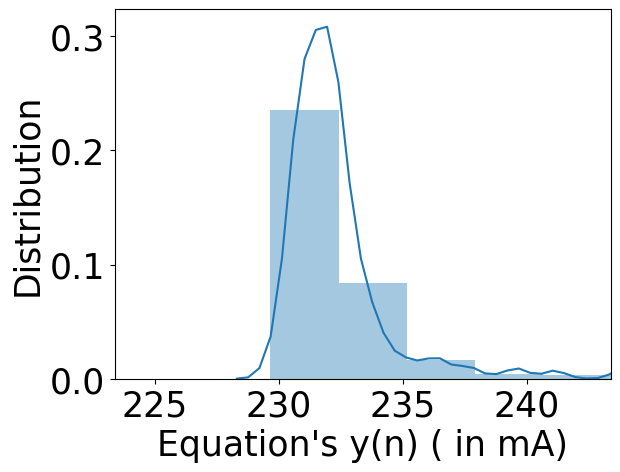
\includegraphics[width=\textwidth]{figures/004_Pixel4_bricksbreaker_menu_250_1_distribution_y_n.png}
%          \caption{250 1-second equations}
%     \end{subfigure}
%     \hfill
%     \begin{subfigure}[b]{0.49\columnwidth}
%          \centering
%          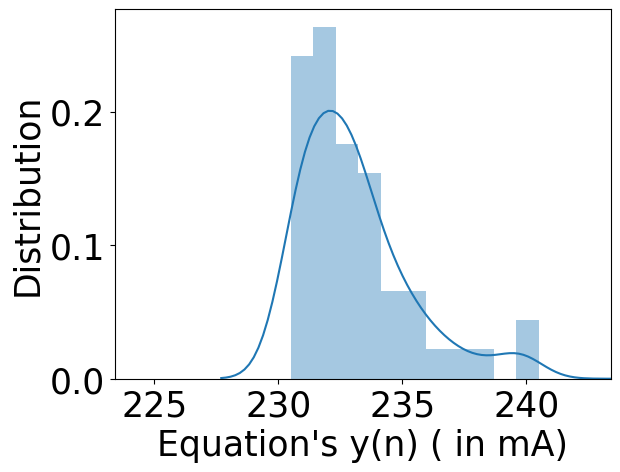
\includegraphics[width=\textwidth]{figures/004_Pixel4_bricksbreaker_menu_250_5_distribution_y_n.png}
%          \caption{50 5-second equations}
%     \end{subfigure}
%     \vspace{-0.1in}
%     \caption{Distribution of the energy terms of the
%     equations for Bricks Breaker Menu scenarios on Pixel 4.}
%     \label{fig:y_distribution}
%     \vspace{-0.2in}
% \end{figure}

\st{To understand why the system of model equations for the 6 app scenarios lack
diversity}{\color{blue}To illustrate the similarity among equations of 1-second interval}, we zoom into the power monitor readings.
Figure~\ref{fig:power_trace_candycrush_menu} shows a snippet of the power monitor
readings during the Candy Crush Saga Menu scenario. We see that the power draw
shows a clear repeating pattern at every 16.7ms interval. This happens due to
typical game app behavior -- a game app typically renders 60 FPS and the graphic
contents rendered within each game scenario are largely similar. As a result,
aggregating the power activities within each of the 1-second interval into one
model equation will result in the set of equations (for the same app scenario)
looking largely similar.

{\color{blue}To summarize, due to the lack of variation of CPU/GPU utilization level in the second-scale, the linear regression used for SPMD becomes very sensitive to the noise and consequently make the modeling results invalid.}

% \comment{To summarize, our experimental results and analysis above suggest that
% the equations created from macro-scale SPMD do not exhibit enough
% diversity and as a result the regression solver even after careful
% adjustments can not output meaningful solutions for the model
% parameters.
% ???
% }

\section{Can Zooming into Smaller Time Scale Improve Diversity?}
\label{sec:micronano}

% \comment{For micro and nano analysis, on a per rendering
%  interval basis, we scale the rendering interval duration from the power
%  monitor trace to match that of the rendering interval duration of the event
%  trace interval on a per interval basis.}

Performing SPMD by setting up equations at the millisecond scale discussed below
require aligning the power event trace and the power monitor trace at the millisecond scale,
as discussed in \S\ref{subsec:align}.

\subsection{Per-Component SPMD at Micro-Scale}
\label{sec:modelling_micro}

%% 1. Introduction: Zooming into 16.7 ms to extract variation
%%    1a. Explain the variation in 16.7 ms: Busy and idle period
%% 2. Explain how the equations are generated
%% 3. Explain the results
%%    3a. Explain why the solution are not correct
%% 4. Provide the reason for the bad solutions: explain underdetermined equations
%%    4a. Explain 2 variable in GPU
%%    4b. Explain 2 variable in CPU
%%    4c. Explain 4 variable 2 equations
%% 5. Conclusion: Due to underdetermined equations, the solution is infeasible

The repeating app usage across rendering intervals suggests that we
need to zoom into each rendering interval in order to create
multiple equations that are diverse in phone component usage.
Figure~\ref{fig:power_trace_candycrush_menu} shows the power draw
during two 16.7 ms intervals for the Candy Crush Saga Menu scenario.
We observe that there are two distinctive plateaus in each 
16.7 ms interval. The high one is when the GPU is in the Busy state
and the low plateau is when the GPU is in the Idle state.  These two
plateaus provide us with two sub intervals for generating two diverse
equations.  We denote this approach as {\it SPMD at micro-scale}.
\begin{figure*}[tp]
     \centering
     \begin{subfigure}[b]{\textwidth}
         \centering
         
\includegraphics[width=\textwidth]{figures/label_macro_equations.png}
    \end{subfigure}
    \\
    \hfill
    \centering
     \begin{subfigure}[b]{0.31\textwidth}
         \centering
         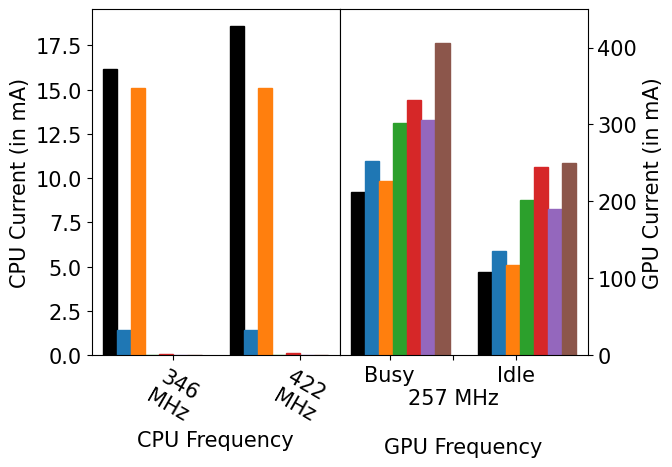
\includegraphics[width=\textwidth]{figures/002_Pixel2_16_micro_equations.png}
         \label{fig:micro_equations_p2}
         \vspace{-0.25in}
         \caption{Pixel 2: TPMD vs micro-SPMD coefficients}
     \end{subfigure}
    \begin{subfigure}[b]{0.32\textwidth}
         \centering
         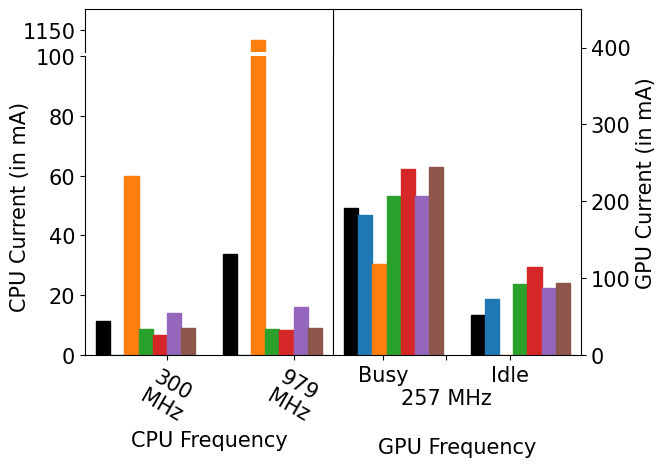
\includegraphics[width=\textwidth]{figures/003_MotoZ3_16_micro_equations.png}
         \label{fig:micro_equations_z3}
         \vspace{-0.25in}
         \caption{Moto Z3: TPMD vs micro-SPMD coefficients}
     \end{subfigure}
    \begin{subfigure}[b]{0.32\textwidth}
         \centering
         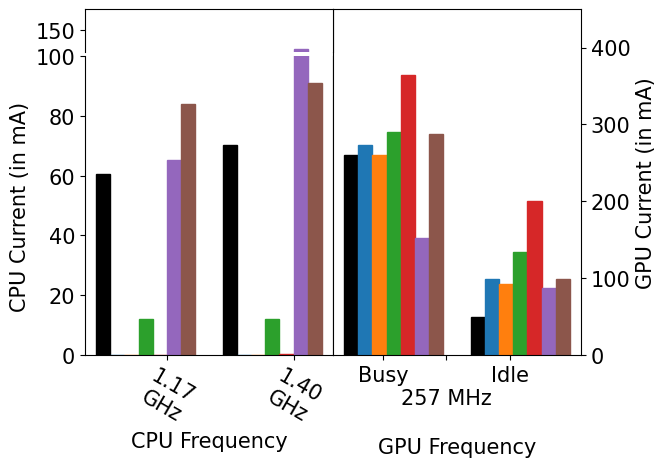
\includegraphics[width=\textwidth]{figures/004_Pixel4_16_micro_equations.png}
         \label{fig:micro_equations_p4}
         \vspace{-0.25in}
         \caption{Pixel 4: TPMD vs micro-SPMD coefficients}
     \end{subfigure}
     \hfill
     \vspace{+0.1in}
     \centering
     \begin{subfigure}[b]{0.31\textwidth}
        \centering
	    \caption{Pixel 2: TPMD vs micro-SPMD error}
	    \vspace{-0.05in}
    	{ \scriptsize
%    	\begin{tabular}{ | p{1.3cm} | p{.2cm} | p{.2cm} | p{.2cm} | p{.2cm} | p{.2cm} | p{.2cm} | }
        \begin{tabular}{ | p{1.8cm} | p{.2cm} | p{.2cm} | p{.2cm} | p{.2cm} | p{.2cm} | p{.2cm} | }
%    	\begin{tabular}{ | l | c | c | c | c | c | c | }
    		\hline
    		     & \multicolumn{6}{ c|}{Error for each App Sc. (\%)}\\
    		\cline{2-7}
                    Model & \rot{B. Menu} & \rot{B. Still} & \rot{C. Menu} & \rot{C. Still} & \rot{M. Menu} & \rot{M. Still}  \\
            \hline
                Fix. F. Const.       & 2.1 & 1.6 & 12 & 13 & 12 & 13 \\
                Classical            & 14 & 25 & 12 & 17 & 13 & 21 \\
            \hline
    	\end{tabular}
    	}
    	% \vspace{-0.05in}
	    % \caption{Pixel 2: TPMD vs micro-SPMD error}
    \end{subfigure}
    \hfill
    \begin{subfigure}[b]{0.31\textwidth}
        \centering
	    \caption{Moto Z3: TPMD vs micro-SPMD error}
	    \vspace{-0.05in}
    	{ \scriptsize
%    	\begin{tabular}{ | p{1.3cm} | p{.2cm} | p{.2cm} | p{.2cm} | p{.2cm} | p{.2cm} | p{.2cm} | }
        \begin{tabular}{ | p{1.8cm} | p{.2cm} | p{.2cm} | p{.2cm} | p{.2cm} | p{.2cm} | p{.2cm} | }
%    	\begin{tabular}{ | l | c | c | c | c | c | c | }
    		\hline
    		     & \multicolumn{6}{ c|}{Error for each App Sc. (\%)}\\
    		\cline{2-7}
                    Model & \rot{B. Menu} & \rot{B. Still} & \rot{C. Menu} & \rot{C. Still} & \rot{M. Menu} & \rot{M. Still}  \\
    		\hline
                Fix. F. Const.       & 7.7 & 16 & 8.5 & 8.1 & 7.4 & 3.6 \\
                Classical            & 30 & 20 & 32 & 19 & 11 & 10 \\
    		\hline
    	\end{tabular}
    	}
    	% \vspace{-0.05in}
	    % \caption{Moto Z3: TPMD vs micro-SPMD error}
    \end{subfigure}
    \hfill
    \begin{subfigure}[b]{0.30\textwidth}
        \centering
	    \caption{Pixel 4: TPMD vs micro-SPMD error}
	    \vspace{-0.05in}
    	{ \scriptsize
%    	\begin{tabular}{ | p{1.3cm} | p{.2cm} | p{.2cm} | p{.2cm} | p{.2cm} | p{.2cm} | p{.2cm} | }
        \begin{tabular}{ | p{1.8cm} | p{.2cm} | p{.2cm} | p{.2cm} | p{.2cm} | p{.2cm} | p{.2cm} | }
%    	\begin{tabular}{ | l | c | c | c | c | c | c | }
    		\hline
    		     & \multicolumn{6}{ c|}{Error for each App Sc. (\%)}\\
    		\cline{2-7}
                    Model & \rot{B. Menu} & \rot{B. Still} & \rot{C. Menu} & \rot{C. Still} & \rot{M. Menu} & \rot{M. Still}  \\
    		\hline
                Fix. F. Const.       & 2.4 & 1.5 & 9.5 & 12 & 3.2 & 6.4 \\
                Classical            & 31 & 35 & 27 & 33 & 20 & 12 \\
    		\hline
    	\end{tabular}
    	}
    	% \vspace{-0.05in}
	    % \caption{Pixel 4: TPMD vs micro-SPMD error}
    \end{subfigure}
    \vspace{-0.1in}
    \caption{Model parameters derived by 8 consecutive 16.7 ms intervals micro-scale SPMD. (Showing the top 2 CPU
        frequencies with high CPU utilization.)(The GPU parameter for TPMD
        is represented by average over all app scenarios GPU parameters.) }
    \label{fig:micro_equations}
    \vspace{-0.1in}
\end{figure*}

\paragraph{Methodology.}
We follow the same methodology as described in
\S\ref{sec:modelling_macro} except that we generated two equations per
16.7 ms interval, one for when GPU is in the Busy state and the other for when 
the GPU is in the Idle
state.
\st{As before, we fixed the base power as a constant to avoid the
under-rank problem and use the Fix. F. Const. % Fix-Freq-Constrained
version of the regression solver.}{\color{blue}--!!-Again, remove and replace Fix. F. Const.  because we no long need the rank -!!--}


% \paragraph{Results.}
% In creating the two equations, we observed that there are more than
% two unknowns as elaborated below.  First, we observe that the GPU almost
% never changes frequency within each 16.7ms interval, and hence it
% contributes two unknowns, \ie for the GPU Busy state and Idle state
% power.  Second, the CPU may change frequency, potentially contributing
% multiple CPU power parameters. This makes the system of two equations
% under-determined. To solve this problem, we tried to set up 2 equations 
% per interval for 4, 8, and 16 intervals, Figure~\ref{fig:micro_equations}
% shows the model parameters output by the regression solver for the six app
% scenarios on the three phones for 8 intervals. 
% The results for other intervals are similar and are omitted due to page limit. 

{\color{blue}We report the modeling results in Figure~\ref{fig:micro_equations}.} We make the following observations.
(1) The power models output by the solver have high LSF{\color{blue}-!!-what is LSF?Maybe it's better not using abbreviation-!!-} error,
between 1.56\%-13.28\% for Pixel 2,
between 3.61\%-15.63\% for Moto Z3,
and between 1.50\%-12.22\% for Pixel 4.
(2) The power parameters range between
0.0$\times$-1.08$\times$,
0.0$\times$-5.75$\times$,
0.0$\times$-1.53$\times$ their
counterparts for CPU frequency for the 3 phones.
(3) The individual power parameters range between
1.14$\times$-1.68$\times$,
0.76$\times$-1.44$\times$,
0.74$\times$-1.42$\times$ their
counterparts for GPU Busy frequency and
1.36$\times$-2.06$\times$,
0.0$\times$-9.48$\times$,
1.22$\times$-28.13$\times$ of their
counterparts for GPU Idle frequency \comment{what is frequency-Idle?? FIXED}
in the TPMD model for Pixel
2, Moto Z3, and Pixel 4, respectively. {\color{blue}We also do the F-test and $R^2$-measurement in Table~?? --EXPLAIN THE TESTING RESULT-- 
As we can see, similar to the situation of macro-scale, at micro-scale SPMD modeling results are still not valid for most of the time. Same explanation in the previous section still applies here, i.e., lack of variation makes the regression result sensitive to the noise.}
\comment{
The high error of these model parameters derived with micro-scale SPMD 
suggests that they cannot capture the power state variation well. 
on what criteria in section 3.6?
}

% \paragraph{Validation.}
% \comment{ 
% How often can we get acceptable solutions for systems of 8 equations? 
% Validation of Micro SPMD using interleaved "training" and "testing" data. 
% Pick 16 equations, form training data using odd equations, and testing data using even equations.
% REMOVING THIS. NOT USED ANYMORE.
% }

\begin{table}[tb]
{\footnotesize
    \centering
    \caption{The 2 smallest singular values for the set of equations for micro-scale "Fix-Freq.-Constr. SPMD" for Pixel 4 for 16 equation system of equation.
    (Top 4 singular values are shown.)
    }
    \vspace{-0.1in}
%    \begin{tabular}{|c|p{9mm}|p{4.5mm}|p{4.5mm}|p{4mm}|p{4mm}|p{4mm}|p{4mm}|c|}
    \begin{tabular}{|c|p{10.5mm}|p{7.5mm}|p{7.5mm}|c|c|c|}
    \hline
        App & Scenario & Num. & Num. &  \multicolumn{2}{c|}{Singular}  & $R^{2}$ \\
            &          &  of &   of &  \multicolumn{2}{c|}{Values}  &   \\
            &          & Eqns. & Vars. &  \multicolumn{2}{c|}{}  & \\
        \hline
         \multirow{2}{13mm}{Bricks Breaker} & Menu & 32 & 6  & 0.17  & 0.12 & 0.99 \\
         \cline{2-7}
         & Still &  32 & 6 & 0.80  & 0.08 & 1.00 \\
         \hline
         \multirow{2}{13mm}{Candy Crush S.} & Menu & 32 & 7 & 0.24  & 0.07 & 0.84 \\
         \cline{2-7}
         & Still & 32 & 7 & 0.17  & 0.04 & 0.65 \\
         \hline
        \multirow{2}{13mm}{Mini Golf 3D} & Menu & 32 & 12 & 0.20  & 0.08 & 0.98 \\
        \cline{2-7}
	     & Still & 32 & 6 & 0.20  & 0.17 & 0.96 \\
	     \hline
    \end{tabular}
    \label{tab:micro_rank_singular}
    \vspace{-0.1in}
}
\end{table}
% \paragraph{Analysis.}
% \comment{
% To understand why some systems can generate reasonable models while
% others cannot, \comment{where do we see this???}
% we plot in Table~\ref{tab:micro_rank_singular} the
% rank and top singular values for the 16-equation systems. 
% We see that all the systems are full rank and have the sufficient number of high
% singular values.
% REMOVING THIS. NOT USED ANYMORE.
% }

\begin{table}[tb]
    \centering
    \caption{Equations for the 8 consecutive 16.7 ms intervals for Bricks Breaker Menu scenario on Moto Z3.}
    {\small
    \vspace{-0.1in}
    \begin{tabular}{|c|c|c|c|c|}
        \hline
             Eqn &    y(n) & \multicolumn{1}{c|}{CPU Utilization} & \multicolumn{2}{c|}{GPU Utilization} \\
        \cline{4-5}
             & (mA) & \multicolumn{1}{c|}{} & Busy & Idle \\
            \hline
               1 & 277.8 & 125\% & 100\% &   0\% \\
               2 & 159.1 & 138\% &   0\% & 100\% \\
               \hline
               3 & 268.6 &  52\% & 100\% &   0\% \\
               4 & 179.3 & 119\% &   3\% &  97\% \\
               \hline
               5 & 318.2 &  69\% & 100\% &   0\% \\
               6 & 160.0 & 132\% &   0\% & 100\% \\
               \hline
               7 & 294.4 &  28\% & 100\% &   0\% \\
               8 & 165.5 & 128\% &   0\% & 100\% \\
               \hline
               9 & 224.9 & 123\% & 100\% &   0\% \\
              10 & 160.3 & 129\% &   0\% & 100\% \\
              \hline
              11 & 293.2 &  50\% & 100\% &   0\% \\
              12 & 168.7 & 130\% &   0\% & 100\% \\
              \hline
              13 & 267.4 &  23\% & 100\% &   0\% \\
              14 & 173.3 & 126\% &   0\% & 100\% \\
              \hline
              15 & 251.5 & 102\% & 100\% &   0\% \\
              16 & 159.8 & 134\% &   0\% & 100\% \\

        \hline
    \end{tabular}
    }
    \label{tab:equations_micro}
    \vspace{-0.1in}
\end{table}

To help readers better understand why SPMD is not able to generate reasonable model,
we take a close look at the system of equations.
% Next,
% we take a close look at two systems, one with acceptable and one
% with unacceptable power parameters generated.
Table~\ref{tab:equations_micro} shows the 16 equations for Bricks
Breaker Menu on Moto Z3
where Equations 1, 3, 5 and 7 correspond to the GPU Busy subintervals
and Equations 2, 4, 6 and 8 correspond to the GPU Idle subintervals
within the rendering intervals.

We make two  observations:
(1) the eight equations for GPU Idle subintervals, 2, 4, 6, 8, 10, 12, 14 and 16, are
very similar in GPU usage and the eight equations for GPU Busy
subintervals, 1, 3, 5, 7, 9, 11, 13, and 15, are very similar in GPU usage.
(2) These two groups differ in CPU utilization which are consistent
with their energy values on the LHS.  We see that the noise in
energy values appear to dominate the diversity in CPU usage.  For
example, the CPU utilization of Eq.~9 and Eq.~11 are 123\% and 50\%,
but their normalized energy value are flipped, at 224.9 mA and 293.2 mA,
respectively.  As a result, the solver is not able to generate
meaningful CPU power parameters.
\comment{ how do we explain the
  energy value variation between Eq.~2 and Eq.~4 does not affect the
  solutions here?  }

\dcomment{
We observe that the $R^2$ value varies between 0.37-0.99, 0.65-0.99 and 0.65-1.00 for the
three phones respectively. This shows that for some app scenarios the
curve\_fit can't fit too well.
For example, for Candy Crush Saga Still on Pixel 4
has a $R^2$ value of 0.65 which is reflected in it's average error of 12\%.
The minimum singular value is 0.04,
causing the system susceptibility to
$0.04^{-1}$$\approx$$25\times$ the measurement noise.
The singular value ratio between the largest and smallest is
4.6$\times$-11.0$\times$, 5.1$\times$-12.1$\times$ and
3.4$\times$-16.6$\times$ on the 3 phones.
The the minimum singular values are between
4.5e-17-0.08,
0.12-0.60
and
0.04-0.17 for the 3 phones respectively.
}

\comment{
These results suggest while zooming into rendering intervals increased the diversity of the systems of equations - they are full rank and have good singular values, but the most of the times the solver cannot output reasonable model parameters due to energy value measurement noise. 
} 

\comment{not sure what to conclude here???}
{\color{blue}Although the modeling results at micro-scale is still not satisfactory for practical use, we do observe better F-test and $R^2$-measurement results that those of the macro-scale.}

\subsection{SPMD at Nano-Scale}
\label{sec:modelling_nano}

%% 1. Introduction: How to get more variations
%% 2. How to generate the equations
%% 3. Explain Alignment how power monitor is aligned with event trace
%%    3a. Explain gradient method to align 
%% 4. Explain the results
%%    4a. Explain problems in CPU Base power
%%    4b. Explain problems in per-core CPU power
%%    4c. Explain problems in GPU
%% 5. Reasons for the equation not giving correct solution
%% 6. Conclusion

Given that the {\color{blue}CPU/GPU utilization level variation} seems to mainly exist within
each rendering interval yet creating two equations per interval is
not enough, we next explore setting up multiple equations, each
at an even finer scale, within each 16.7ms interval. We denote this
approach as {\it SPMD at nano-scale}.

\paragraph{Methodology.}
The methodology is similar to that of micro-scale SPMD, except that
instead of generating two equation per 16.7 ms interval, we generate
16 equations, \ie one equation for every 1ms sub-interval.  We tried
to set up one system for 1, 2, 4, and 8 16.7ms intervals and show results for 1
interval, \ie 16 equations.  The other results are
very similar and are omitted due to page limit.
\begin{figure*}[tp]
    \centering
     \begin{subfigure}[b]{\textwidth}
         \centering
         
\includegraphics[width=\textwidth]{figures/label_macro_equations.png}
    \end{subfigure}
    \\
    \centering
     \begin{subfigure}[b]{0.32\textwidth}
         \centering
         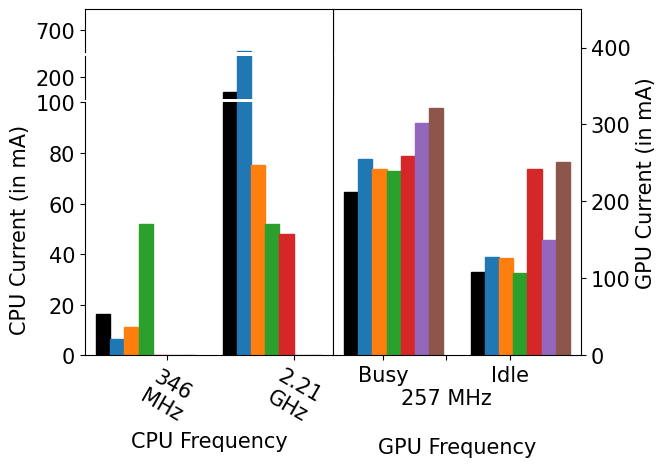
\includegraphics[width=\textwidth]{figures/002_Pixel2_1_nano_equations.png}
         \label{fig:nano_equations_p2}
         \vspace{-0.25in}
         \caption{Pixel 2: TPMD vs nano-SPMD coefficients}
     \end{subfigure}
    \begin{subfigure}[b]{0.32\textwidth}
         \centering
         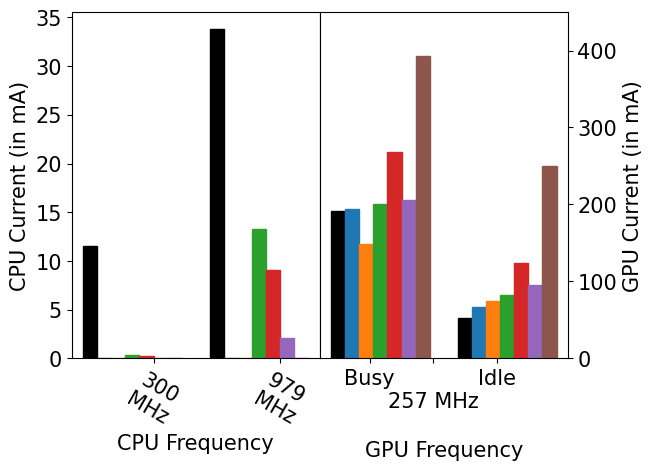
\includegraphics[width=\textwidth]{figures/003_MotoZ3_1_nano_equations.png}
         \label{fig:nano_equations_z3}
         \vspace{-0.25in}
         \caption{Moto Z3: TPMD vs nano-SPMD coefficients}
     \end{subfigure}
    \begin{subfigure}[b]{0.32\textwidth}
         \centering
         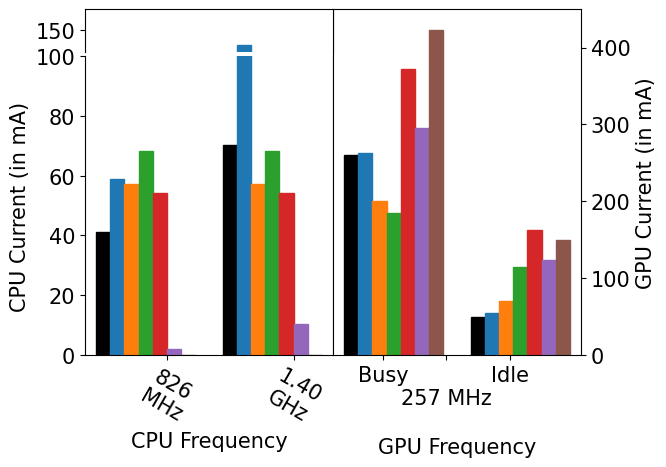
\includegraphics[width=\textwidth]{figures/004_Pixel4_1_nano_equations.png}
         \label{fig:nano_equations_p4}
         \vspace{-0.25in}
         \caption{Pixel 4: TPMD vs nano-SPMD coefficients}
     \end{subfigure}
     \hfill
     \vspace{+0.1in}
     \centering
     \begin{subfigure}[b]{0.31\textwidth}
        \centering
	    \caption{Pixel 2: TPMD vs nano-SPMD error}
	    \vspace{-0.05in}
    	{ \scriptsize
%    	\begin{tabular}{ | p{1.3cm} | p{.2cm} | p{.2cm} | p{.2cm} | p{.2cm} | p{.2cm} | p{.2cm} | }
        \begin{tabular}{ | p{1.8cm} | p{.2cm} | p{.2cm} | p{.2cm} | p{.2cm} | p{.2cm} | p{.2cm} | }
%    	\begin{tabular}{ | l | c | c | c | c | c | c | }
    		\hline
    		     & \multicolumn{6}{ c|}{Error for each App Sc. (\%)}\\
    		\cline{2-7}
                    Model & \rot{B. Menu} & \rot{B. Still} & \rot{C. Menu} & \rot{C. Still} & \rot{M. Menu} & \rot{M. Still}  \\
    		\hline
                Fix. F. Const.       & 4.3 & 3.8 & 12 & 9.1 & 13 & 16 \\
                TPMD                 & 19 & 30 & 23 & 22 & 22 & 31 \\
    		\hline
    	\end{tabular}
    	}
    	% \vspace{-0.05in}
	    % \caption{Pixel 2: TPMD vs nano-SPMD error}
    \end{subfigure}
    \hfill
    \begin{subfigure}[b]{0.31\textwidth}
        \centering
	    \caption{Moto Z3: TPMD vs nano-SPMD error}
	    \vspace{-0.05in}
    	{ \scriptsize
%    	\begin{tabular}{ | p{1.3cm} | p{.2cm} | p{.2cm} | p{.2cm} | p{.2cm} | p{.2cm} | p{.2cm} | }
        \begin{tabular}{ | p{1.8cm} | p{.2cm} | p{.2cm} | p{.2cm} | p{.2cm} | p{.2cm} | p{.2cm} | }
%    	\begin{tabular}{ | l | c | c | c | c | c | c | }
    		\hline
    		     & \multicolumn{6}{ c|}{Error for each App Sc. (\%)}\\
    		\cline{2-7}
                    Model & \rot{B. Menu} & \rot{B. Still} & \rot{C. Menu} & \rot{C. Still} & \rot{M. Menu} & \rot{M. Still}  \\
    		\hline
                Fix. F. Const.       & 14 & 14 & 7.3 & 14 & 21 & 7.8 \\
                TPMD                 & 42 & 18 & 39 & 27 & 41 & 41 \\
    		\hline
    	\end{tabular}
    	}
    	% \vspace{-0.05in}
	    % \caption{Moto Z3: TPMD vs nano-SPMD error}
    \end{subfigure}
    \hfill
    \begin{subfigure}[b]{0.31\textwidth}
        \centering
    	\caption{Pixel 4: TPMD vs nano-SPMD error}
    	\vspace{-0.05in}
    	{ \scriptsize
%    	\begin{tabular}{ | p{1.3cm} | p{.2cm} | p{.2cm} | p{.2cm} | p{.2cm} | p{.2cm} | p{.2cm} | }
        \begin{tabular}{ | p{1.8cm} | p{.2cm} | p{.2cm} | p{.2cm} | p{.2cm} | p{.2cm} | p{.2cm} | }
%    	\begin{tabular}{ | l | c | c | c | c | c | c | }
    		\hline
    		     & \multicolumn{6}{ c|}{Error for each App Sc. (\%)}\\
    		\cline{2-7}
                    Model & \rot{B. Menu} & \rot{B. Still} & \rot{C. Menu} & \rot{C. Still} & \rot{M. Menu} & \rot{M. Still}  \\
    		\hline
                Fix. F. Const.       & 13 & 11 & 16 & 27 & 21 & 26 \\
                TPMD                 & 38 & 50 & 23 & 42 & 29 & 34 \\
    		\hline
    	\end{tabular}
    	}
    	% \vspace{-0.05in}
    	% \caption{Pixel 4: TPMD vs nano-SPMD error}
    \end{subfigure}
    \hfill
    \caption{Model parameters derived by nano-scale SPMD. (Showing the top 2 CPU
        frequencies with high CPU utilization.)(The GPU parameter for the TPMD
        is represented by average over all app scenarios GPU parameters.) }
    \vspace{-0.1in}
    \label{fig:nano_equations}
\end{figure*}

\paragraph{Results.}
Figure~\ref{fig:nano_equations} shows the model parameters output of the 
Fix. F. Const. regression solver for the same 6 app scenarios.  We
observe that the model parameters derived from nano-scale SPMD are
also drastically different from the corresponding parameters derived
from the TPMD model.  In particular, 
(1) the power models output
by the solver have high LSF error,
between (3.75\%-16.40\%) for Pixel 2,
between (7.29\%-20.61\%) for Moto Z3,
and between (11.28\%-26.58\%) for Pixel 4;
% (2) For Pixel 4, out of the 6 app scenarios, the CPU parameters are zero for 2
%  scenarios and less than 50\% of the TPMD counterparts for 3
%  scenarios.  Similarly, the CPU parameters are zero for 2 scenarios and
%  less than 50\% of thei TPMD counterprts for 4 scenarios for
%  Moto Z3.  Finally, the CPU parameters are zero \comment{for all scenarios???} for Pixel 2.
(2) the power parameters are
0.0$\times$-2.76$\times$,
0.0$\times$-0.57$\times$,
0.0$\times$-1.62$\times$ of their
counterparts for CPU frequency respectively for the 3 phones; and
(3) the individual power parameters are
1.02$\times$-1.48$\times$,
0.78$\times$-1.92$\times$,
0.50$\times$-1.43$\times$ of their
counterparts for GPU Busy frequency and
0.72$\times$-2.08$\times$,
0.74$\times$-8.60$\times$,
1.09$\times$-21.60$\times$ of their
counterparts for GPU Idle frequency in the TPMD model for Pixel 2,
Moto Z3, and Pixel 4, respectively.
 
 \comment{so,do we reject these results? on what basis? need to echo section 3.4}
 
{\color{blue}We report the corresponding  $R^2$-measurement and F-test in Table~\ref{tab:nano_rank_singular}.--EXPLAIN THOSE VALUES-- Still SMPD does not give a reasonable valid modeling results.}
\dcomment{
We observe that the $R^2$ varies between 0.25-0.96, 0.34-0.95 and 0.63-0.93 for the
three phones respectively. Similar to micro, we observe that for some app scenarios the
curve\_fit fail \eg for Candy Crush Still on Pixel 4 has the lowest 
$R^2$ value of 0.63. It's has the highest average error of 27\%.
and having the minimum singular value was 0.39. 
Here the system's susceptibility to noise can be
estimated to be $0.39^{-1} \approx 2.6\times$ the measurement noise.
% From $\|\epsilon_m\|_2/\min\text{eig}(\mathbf{X})$, explained in
% \S\ref{subsec:contri} NEED TO CONCLUDE.
The the minimum singular values are between
0.20-0.77,
0.50-0.91
and
0.29-1.07 for the 3 phones respectively.
} 
 
\begin{table}[tb]
{\footnotesize
    \centering
    \caption{The 2 smallest singular values for the set of equations for nano-scale "Fix-Freq.-Constr. SPMD" for Pixel 4  for 16 equation system of equation.
    (Top 4 singular values are shown.)
    }
    \vspace{-0.1in}
    % \begin{tabular}{|c|p{9mm}|p{4.5mm}|p{4.5mm}|p{4mm}|p{4mm}|p{4mm}|c|}
    % \hline
    %     App & Scenario & Num. of Eqns. & Num. of Vars. &  \multicolumn{3}{c|}{Smallest Singular Values} & $R^{2}$ \\
    \begin{tabular}{|c|p{10.5mm}|p{7.5mm}|p{7.5mm}|c|c|c|}
    \hline
        App & Scenario & Num. & Num. &  \multicolumn{2}{c|}{Singular}  & $R^{2}$ \\
            &          &  of &   of &  \multicolumn{2}{c|}{Values}  &   \\
            &          & Eqns. & Vars. &  \multicolumn{2}{c|}{}  & \\
        \hline
        \multirow{2}{13mm}{Bricks Breaker} & Menu & 16 & 4  & 1.42  & 1.07 & 0.93 \\
         \cline{2-7}
         & Still & 16 & 4 & 1.31  & 1.01 & 0.87 \\
         \hline
        \multirow{2}{13mm}{Candy Crush S.} & Menu & 16 & 4  & 1.25 & 0.29 & 0.81 \\
        \cline{2-7}
	     & Still & 16 & 4 & 0.87  & 0.39 & 0.63 \\
	     \hline
         \multirow{2}{13mm}{Mini Golf 3D} & Menu & 16 & 5 & 1.68  & 0.51 & 0.73 \\
         \cline{2-7}
         & Still & 16 & 5 & 0.75 & 0.48 & 0.77 \\
         \hline
    \end{tabular}
    \label{tab:nano_rank_singular}
    \vspace{-0.1in}
}
\end{table}

\begin{table}[tb]
    \centering
    \caption{Equations for the 16.7 ms interval for Bricks Breaker Menu scenario on Moto Z3 for 16 equation set.}
    {\small
    \begin{tabular}{|c|c|c|c|c|}
        \hline
            Eqn & y(n) & \multicolumn{1}{c|}{CPU Utilization} & \multicolumn{2}{c|}{GPU Utilization} \\
        \cline{4-5}
            & (mA) & \multicolumn{1}{c|}{} & Busy & Idle \\
        \hline
               1 & 339.4 & 111\% & 100\% &   0\% \\
               2 & 326.3 & 124\% & 100\% &   0\% \\
               3 & 177.9 & 145\% &  94\% &   6\% \\
               4 & 156.0 & 190\% &   0\% & 100\% \\
               5 & 144.0 & 169\% &   0\% & 100\% \\
               6 & 159.6 & 118\% &   0\% & 100\% \\
               7 & 160.6 & 128\% &   0\% & 100\% \\
               8 & 169.6 & 164\% &   0\% & 100\% \\
               9 & 173.5 & 156\% &   0\% & 100\% \\
              10 & 161.3 & 100\% &   0\% & 100\% \\
              11 & 158.7 & 100\% &   0\% & 100\% \\
              12 & 165.5 & 114\% &   0\% & 100\% \\
              13 & 164.3 & 115\% &   0\% & 100\% \\
              14 & 163.3 & 193\% &   0\% & 100\% \\
              15 & 140.4 & 122\% &   0\% & 100\% \\
              16 & 146.8 & 116\% &   0\% & 100\% \\
        \hline
    \end{tabular}
    }
    \label{tab:equations_nano}
    \vspace{-0.1in}
\end{table}

% \paragraph{Analysis.}
% Table~\ref{tab:nano_rank_singular} shows the systems of equations are full rank and have reasonable singular values for Moto Z3. 

Finally, we looked into the individual equations to understand why
nano-scale SPMD cannot output accurate model parameters. % ither.
Table~\ref{tab:equations_nano} shows the 16 equations for the 16.7ms
interval for the Bricks Breaker Menu scenario on Moto Z3. We make two
observations.  (1) The equations fall into two groups, corresponding
to the GPU Busy state (\ie Eq.~1 and Eq.~2) and Idle state (\ie Eq.~4 to Eq.~16)
with Eq.~3 corresponding to the transition from Busy to Idle.
(2) Within each group, many equations contradict each other.
For example, the CPU utilization in the GPU Idle group, Eq.~8 are higher than
those in Eq.~9 yet the LHS energy values are the opposite. The same
happens for GPU Busy group, \eg between Eq.~1 and Eq.~2. These numbers
suggest that again the 16 equations \dcomment {\st{not only}} did not add {\color{blue}too much variation of CPU/GPU utilization}, but actually added noise to the equations making it hard
for the solver to output meaningful model parameters.

%% 6. Conclusion
To summarize, the above experiments and analysis suggest that nano-scale SMPD, \ie
creating equations at 1ms granularity, is also impractical to derive
meaningful model parameters.

{\color{blue}By comparing the $R^2$ values for different scales, we find an interesting phenomenon that the micro-scale is better than the nano-scale, and the nano-scale is better than the macro-scale. This phenomenon shows that a carefully-chosen granularity may helps to reduce the effect of noise and produce reliable modeling results.}

\begin{table*}[tb]
\centering
{\footnotesize
    \centering
    \caption{(This table will be remove and absorbed into singular value table.) The $R^{2}$ and ANOVA F one way test between y and $y_{pred}$.
    \dcomment{Should we remove F-test analysis?}
    }
    % \vspace{-0.1in}
    \begin{tabular}{|p{12mm}|p{9.5mm}|p{4mm}|p{9.5mm}|p{2.5mm}|p{4mm}|p{4mm}|p{4mm}|p{9.5mm}|p{2.5mm}|p{4mm}|p{4mm}|p{4mm}|p{9.5mm}|p{2.5mm}|p{4mm}|p{4mm}|}
    \hline
        App & Scenario & \multicolumn{15}{c|}{F-Test} \\
        \cline{3-17}
        & & \multicolumn{5}{c|}{Macro-SMPD} & \multicolumn{5}{c|}{Micro-SMPD} & \multicolumn{5}{c|}{Nano-SMPD} \\
        \cline{3-17}
        & & $R^{2}$ & F & p & $F_{C}$ & $F_{C}$ & $R^{2}$ & F & p & $F_{C}$ & $F_{C}$ & $R^{2}$ & F & p & $F_{C}$ & $F_{C}$ \\
        & & & & & \scriptsize{$\alpha=0.05$} & \scriptsize{$\alpha=0.10$} & & & & \scriptsize{$\alpha=0.05$} & \scriptsize{$\alpha=0.10$} & & & & \scriptsize{$\alpha=0.05$} & \scriptsize{$\alpha=0.10$} \\
        \hline
        \multirow{2}{13mm}{Bricks Breaker} & Menu & 0.68 & 7.8E-17 &  1.0 & \multirow{6}{2mm}{3.94} & \multirow{6}{2mm}{2.76}        & 0.99 & 1.4E-20 &  1.0 & \multirow{6}{2mm}{3.99} & \multirow{6}{2mm}{2.79}        & 0.93 & 5.4E-18 &  1.0 & \multirow{6}{2mm}{4.16} & \multirow{6}{2mm}{2.87}       \\
        \cline{2-5}
        \cline{8-10}
        \cline{13-15}
         & Still & 0.83 & 1.1E-17 &  1.0 &      &             & 1.00 & 3.8E-19 &  1.0 &      &             & 0.87 & 4.1E-19 &  1.0 &      &            \\
        \cline{1-5}
        \cline{8-10}
        \cline{13-15}
        \multirow{2}{13mm}{Candy Crush S.} & Menu & 0.73 & 4.9E-17 &  1.0 &      &             & 0.84 & 2.5E-18 &  1.0 &      &             & 0.81 & 5.0E-19 &  1.0 &      &            \\
        \cline{2-5}
        \cline{8-10}
        \cline{13-15}
	     & Still & 0.47 & 3.4E-17 &  1.0 &      &             & 0.65 & 4.4E-18 &  1.0 &      &             & 0.63 & 6.6E-18 &  1.0 &      &            \\
	    \cline{1-5}
        \cline{8-10}
        \cline{13-15}
        \multirow{2}{13mm}{Mini Golf 3D} & Menu & 0.80 & 3.6E-17 &  1.0 &      &             & 0.98 & 5.1E-19 &  1.0 &      &             & 0.73 & 2.8E-21 &  1.0 &      &            \\
        \cline{2-5}
        \cline{8-10}
        \cline{13-15}
         & Still & 0.89 & 4.4E-17 &  1.0 &      &             & 0.96 & 2.4E-19 &  1.0 &      &             & 0.77 & 1.8E-19 &  1.0 &      &            \\
        \hline
    \end{tabular}
    \label{tab:test_table}
    \vspace{-0.1in}
}
\end{table*}
\section{Related Work}
\label{sec:related}

The large amount of prior work on power modeling can be categorized along three dimensions: 
model type, using external power monitor or self-metering, and model derivation process.

\paragraph{Utilization-based vs. FSM-based power models.} 
The large number of power models for different components of
smartphones can be grouped into two categories based on the way they
capture two different types of phone component power draw behaviors.
The first category of power models known as utilization-based models
(\eg \cite{shye2009into,zhang2010accurate,hotpowermulticore}) captures
the synchronous power draw behavior of components; where a hardware
component enters a certain power state and draws power for the
duration when it is actively used in that state, \eg the CPU running
at 2 GHz
% and change of utilization is what triggers the power state change of that component. 
Consequently, these models use the utilization of a hardware component as an input to the power models.
% ``trigger'' in modeling power states and state transitions.  

% Such models thus do not capture power behavior of
% modern wireless components that do not lead to active utilization such
% as the promotion and tail power behavior of 3G and
% LTE~\cite{rrc:imc2010,4glte}, and thus can incur high modeling error.

The second category known as non-utilization-based power models captures the asynchronous power 
draw behavior of hardware components where an app’s usage of a phone component
triggers that component to enter some power state and continues even beyond the duration of the app usage.
Non-utilization-based models capture such power behavior using finite state machines (FSMs),
\eg \cite{arunabimc09,energybasedRA,aro,whatsup:mobicom12,pathak:eurosys12,ding:sigmetrics13}
for WiFi, 3G and~\cite{4glte} for 4G/LTE. 
To derive such models, the built-in state machine of such hardware components, \eg the RRC states and
transitions in the LTE radio, is reverse-engineered and represented in an FSM
annotated with app utilization, \eg either packet-level traces~\cite{rrc:imc2010,4glte} or
networking system calls~\cite{pathak:eurosys12}, as the triggers for the state transitions.

\paragraph{Using external power monitor vs. self-metering.}
Deriving the power models of a mobile device 
requires ground-truth power draw measurement, whether it is for one component as in case of TPMD or for several components as a whole as in case of SPMD. This can be done using an external power monitor such as Monsoon~\cite{powermonitor} or
using energy information from the built-in battery interface. 

PowerBooter~\cite{powerbooter:2010} proposed to use battery
State-of-Charge (SoD) readings to infer the average power draw which has a
very long generation time.
%
Sesame~\cite{sesame:2011} uses drop in the battery capacity during a
sampling interval to infer the average power draw but it shows a high
error at 0.1 Hz.
% 
V-edge~\cite{vedge:2013} exploits the correlation between change in
current and voltage to extrapolate power draw (relative to a baseline)
using only voltage readings.  DevScope~\cite{devscope:2012} studies
the approach to overcome the coarse granularity of current sensor
readings to derive power models for a single component at a time.
%
Since Android 6, Android phones provided interfaces for power and
energy readings which however come with limited accuracy as discussed
in \S\ref{subsec:modelling_sensor}.



\paragraph{TPMD vs. SPMD.}
The third dimension of power modeling is whether to derive the model of one phone component state at a time by isolating the measured power for each of the component state as in case of TPMD, or 
to derive the model for all the component states by solving a system of equations as in case of SPMD, as already discussed in \S\ref{subsec:back}.

\section{Conclusion}
\label{sec:conc}

In this paper, we performed an in-depth study of the feasibility of
self-constructive per-component power model derivation (SPMD) on
modern smartphones. {\color{blue}Although our experiment results show that SMPD cannot always produce reasonable modeling results due the existence of noise, we show a detailed process of implementing SMPD on modern smartphones. Meanwhile, we also provide useful guidance to improve the performance of SMPD by choosing suitable granularity to exploit the variation of the utilization level of CPU/GPU.}
\st{Using three representative phones, we identified the
equation diversity as the primary challenge of SPMD and explored
diverse time-scales in trying to create equations that exhibit high
diversity.  Our experiments and analysis have shown that it is
extremely difficult to create a system of equations with sufficient diversity for
the regression solver to generate meaningful per-component power model
parameters.  Our feasibility study debunked a myth about the
applicability of SPMD at the per-component level of modern smartphones.}

\bibliographystyle{abbrv}
% \bibliography{ref}
\bibliography{mobile}

% \section*{Appendix: Results for Nexus 6 }
%%%%%%%%%%%%%%%% Micro scale

The GPU in Nexus 6 can run at 5 different frequencies and three power states; Active, Init and Nap. Init corresponds to Aware and Nap corresponds to Slumber of Moto Z3.

Since Nexus 6 has a weaker GPU, Boat Racing ran with average GPU utilization close to 100\%
% 95.6\%
and barely entering the GPU Idle state.
Thus we used Bricks Breaker and Candy Crush Saga for Nexus 6 experiments 
which had an average GPU utilization of 77.01\% and 61.82\% respectively.

For Nexus 6, the game apps run with high GPU utilization causing the phone temperature to increase. 
To prevent the phone from switching off cores during app runs due to thermal throttling,
we performed SPMD modeling on Nexus 6 with only 2 CPU cores turned on.


\paragraph{Freq-constrained SPMD} 
For Nexus 6, when we model the core power as a polynomial of frequency, 
we found the fitted exponent $n$ for 1, 2 and 4 cores to be {1.85, 2.04 and 2.25, respectively}. 
Therefore we model the Nexus 6 core as a second-order polynomial of CPU frequency.
\comment{which exponent?}

\subsection*{A1. GPU Power Model is App Dependent for Nexus 6}
\begin{table*}[tp]
{\footnotesize
    \centering
    \caption{Nexus 6 GPU power model (active-busy and active-idle power per frequency) with the CPU fixed at 1.037 GHz.}
    \vspace{-0.1in}
    \begin{tabular}{|p{15mm}|p{9mm}|c|c|c|c|c|c|c|c|c|c|}
    \hline
    App & Scenario & \multicolumn{10}{c|}{GPU Frequency} \\
    \cline{3-12}
     &  & \multicolumn{2}{c|}{240 MHz} & \multicolumn{2}{c|}{300 MHz} & \multicolumn{2}{c|}{389 MHz} & \multicolumn{2}{c|}{500 MHz} & \multicolumn{2}{c|}{600 MHz} \\
     \cline{3-12}
     & & Busy & Idle & Busy & Idle & Busy & Idle & Busy & Idle & Busy & Idle \\
    \hline
      \multirow{2}{15mm}{Candy Crush Saga}  & Intro & 387.4 & 378.9 & 520.3 & 390.9 & 640.0 & 432.9 & 880.3 & 408.3 & 1387.2 & 378.9 \\
      \cline{2-12}
         & Tutorial & 625.4 & 747.0 & 375.0 & 908.2 & 790.8 & 523.4 & 1022.0 & 493.4 & 1211.4 & 602.4 \\
         \hline
        \multirow{2}{13mm}{Bricks Breaker}  & Into & 411.2 & 261.0 & 498.2 & 193.6 & 596.9 & 254.7 & 817.2 & 298.7 & 1181.3 & 410.7 \\
        \cline{2-12}
         & Still & 387.7 & 348.6 & 635.5 & 373.3 & 553.9 & 260.5 & 757.4 & 292.5 & 994.2 & 420.7 \\
         \hline
    \end{tabular}
    \label{tab:gpumodel_nexus6}
    \vspace{-0.1in}
    }
\end{table*}

\subsection*{A2. Model Parameters by Macro-scale SPMD for Nexus 6}
\begin{table*}[tp]
\caption{Model parameters derived by macro-scale SPMD for Nexus 6. The classic models for GPU are from Table~\ref{tab:gpumodel_nexus6}. (Only model parameters for 3 CPU frequencies with highest utilization are shown due to space constraint.)}
\vspace{-0.1in}
{\footnotesize
    \begin{tabular}{|c|c|c|c|c|c|c|c|c|c|}
    \hline
        Model & Base & \multicolumn{3}{c|}{CPU Frequency} & \multicolumn{4}{c|}{GPU Frequency} & Error \\
    \cline{3-9}
        & & \multicolumn{3}{c|}{} & Busy & Idle & Busy & Idle & (\%) \\
    \hline
    \multicolumn{10}{|c|}{\bf Candy Crush Saga Intro Scenario} \\
        \hline
        &  & 730 MHz & 1.27 GHz & 1.57 GHz & \multicolumn{2}{c|}{240 MHz} & \multicolumn{2}{c|}{300 MHz} & \\
        \hline
        Unconstr. SPMD & -134.6 & 3.46 & 81.70 & 232.8 & 545.5 & 325.5 & 933.9 & 150.5 & 0.92 \\
        Constr. SPMD & 0.00 & 39.52 & 111.3 & 228.3 & 544.8 & 5.79 & 698.9 & 5.79 & 1.17 \\
        Freq-Constr. SPMD& 3.62 & 46.73 & 141.0 & 217.6 & 524.7 & 0.00 & 819.8 & 0.00 & 1.55 \\
        \hline
        Classical & 20.16 & 53.35 & 138.0 & 186.5 & 387.4 & 378.9 & 520.3 & 390.9 & 43.50 \\
        \hline

    \multicolumn{10}{|c|}{\bf Candy Crush Saga Tutorial Scenario} \\
        \hline
        &  & 730 MHz & 960 MHz & 1.27 GHz & \multicolumn{2}{c|}{240 MHz} & \multicolumn{2}{c|}{300 MHz} & \\
        \hline
        Unconstr. SPMD & 17209948.0 & 339.8 & 550.3 & 246.5 & -17209018.0 & -17209618.0 & -17209370.3 & -17209132.4 & 4.76 \\
        Constr. SPMD & 258.0 & 53.48 & 53.48 & 53.48 & 143.0 & 103.8 & 168.3 & 129.2 & 4.97 \\
        Freq-Constr. SPMD& 517.6 & 0.00 & 0.00 & 0.00 & 23.18 & 23.18 & 36.22 & 36.22 & 4.96 \\
        \hline
        Classical & 20.16 & 53.35 & 107.1 & 138.0 & 625.4 & 747.0 & 375.0 & 908.2 & 158.4 \\
        \hline

        
    \multicolumn{10}{|c|}{\bf Break Breakers Into Scenario} \\
        \hline
        &  & 960 MHz & 1.27 GHz & 1.57 GHz & \multicolumn{2}{c|}{240 MHz} & \multicolumn{2}{c|}{300 MHz} & \\
        \hline
        Unconstr. SPMD & -57.12 & -607.1 & -55.5 & -1444.0 & 356.4 & 937.5 & 469.6 & 774.4 & 2.63 \\
        Constr. SPMD & 358.2 & 15.69 & 15.69 & 15.69 & 0.36 & 0.36 & 75.24 & 0.36 & 2.78 \\
        Freq-Constr. SPMD& 274.9 & 0.00 & 0.00 & 0.00 & 90.44 & 90.44 & 141.3 & 141.3 & 2.81 \\
        \hline
        Classical & 20.16 & 107.1 & 138.0 & 186.5 & 411.2 & 261.0 & 498.2 & 193.6 & 22.66 \\
        \hline

    \multicolumn{10}{|c|}{\bf Break Breakers Still Scenario} \\
        \hline
        &  & 1.04 GHz & 1.27 GHz & 1.57 GHz & \multicolumn{2}{c|}{240 MHz} & \multicolumn{2}{c|}{-} & \\
       \hline
        Unconstr. SPMD & 366.2 & 216.2 & 201.0 & 236.5 & -0.13 & -23.17 & - & - & 0.55 \\
        Constr. SPMD & 70.35 & 161.5 & 161.5 & 282.9 & 263.1 & 212.6 & - & - & 0.63 \\
        Freq-Constr. SPMD& 222.3 & 101.6 & 151.8 & 234.3 & 77.45 & 61.03 & - & - & 0.72 \\
        \hline
        Classical & 20.16 & 114.4 & 138.0 & 186.5 & 387.7 & 348.6 & - & - & 34.65 \\
        \hline

\end{tabular}
}
\label{tab:nexus6macro}
\vspace{-0.1in}
\end{table*}

\begin{table*}[tp]
% \questionaj{Also add rank of freq-constrained case}
{\small
    \centering
    \caption{The rank and singular values for the set of equations for macro-scale SPMD for Nexus 6.}
    \vspace{-0.1in}
    \begin{tabular}{|c|c|c|c|c|c|c|c|c|c|c|c|c|c|c|c|}
    \hline
        App & Scenario & \# of Eqns. & \# of Vars. & Rank &  \multicolumn{11}{c|}{Singular Values} \\
        \hline
        \multirow{2}{15mm}{Candy Crush Saga} & Into & 100 & 17 & 16 & 13.00  & 1.86  & 0.75  & 0.62  & 0.59  & 0.50  & 0.49  & 0.44  & 0.37  & 0.32  & 0.30 \\
        \cline{2-16}
	     & Tutorial &  100 & 18 & 18 & 28.76  & 1.74  & 1.23  & 0.69  & 0.47  & 0.32  & 0.28  & 0.24  & 0.22  & 0.20  & 0.16\\
	     \hline
	     \multirow{2}{15mm}{Bricks Breaker} & Into & 100 & 15 & 13 & 13.98  & 1.89  & 0.65  & 0.51  & 0.45  & 0.29  & 0.17  & 0.12  & 0.08  & 0.04  & 0.04 \\
         \cline{2-16}
         & Still & 100 & 15 & 14 & 14.26  & 1.06  & 0.48  & 0.35  & 0.30  & 0.22  & 0.18  & 0.11  & 0.06  & 0.05  & 0.05 \\
         \hline
    \end{tabular}
    \label{tab:macro_singularvalues_nexus6}
    \vspace{-0.1in}
}
\end{table*}

\subsection*{A3. Model Parameters by Micro-scale SPMD for Nexus 6}
The solution for Micro-scale SPMD for Nexus 6 is shown in Table~\ref{tab:nexus6micro}.
\begin{table*}[tp]
\caption{Model parameters derived by micro-scale SPMD For Nexus 6.}
\vspace{-0.1in}
{\footnotesize
    \begin{tabular}{|c|c|c|c|c|p{5.4mm}|}
    \hline
        Model & Base & \multicolumn{1}{c|}{CPU Frequency} & \multicolumn{2}{c|}{GPU Frequency} & Error \\
    \cline{3-5}
        & & \multicolumn{1}{c|}{} & Busy & Idle & (in\%) \\
    \hline
    \multicolumn{6}{|c|}{\textbf{Candy Crush Saga Intro Scenario}} \\
        \hline
        &  & 1.19 GHz & \multicolumn{2}{c|}{240 MHz} & \\
        \hline
        % Unconstrained & 200.45 & -3.53 & 446.33 & 426.98 & 0.16 \\
        % Constrained & 623.96 & 0.00 & 21.54 & 0.00 & 0.15 \\
        Freq-Constr. & 419.2 & 0.00 & 226.3 & 204.8 & 0.15 \\
        \hline
        Classical & 20.16 & 130.5 & 387.4 & 378.9 & 23.31 \\
        \hline

    \multicolumn{6}{|c|}{\textbf{Candy Crush Saga Tutorial Scenario}} \\
        \hline
        &  & 422 MHz & \multicolumn{2}{c|}{240 MHz} & \\
        \hline
        % Unconstrained & 98.24 & -60.52 & 462.65 & 352.91 & 13.22 \\
        % Constrained & 45.50 & 0.00 & 467.24 & 367.76 & 14.64 \\
        Freq-Constr. & 413.3 & 0.00 & 99.48 & 0.00 & 14.64 \\
        \hline
        Classical & 20.16 & 32.17 & 625.4 & 747.0 & 64.32 \\
        \hline

    \multicolumn{6}{|c|}{\textbf{Brick Breakers Intro Scenario}} \\
        \hline
        &  & 422 MHz & \multicolumn{2}{c|}{240 MHz} & \\
        \hline
        % Unconstrained & 579.53 & 56.86 & -291.08 & -377.19 & 3.52 \\
        % Constrained & 0.06 & 56.86 & 288.39 & 202.28 & 3.52 \\
        Freq-Constr. & 145.2 & 56.86 & 143.3 & 57.19 & 3.52 \\
        \hline
        Classical & 20.16 & 32.17 & 411.2 & 261.0 & 25.58 \\
        \hline

    \multicolumn{6}{|c|}{\textbf{Brick Breakers Still Scenario}} \\
        \hline
        &  & 422 MHz & \multicolumn{2}{c|}{240 MHz} & \\
        \hline
        % Unconstrained & -125.55 & 8.21 & 428.48 & 426.29 & 3.53 \\
        % Constrained & 200.87 & 8.21 & 102.07 & 99.87 & 3.53 \\
        Freq-Constr. & 300.7 & 8.21 & 2.20 & 0.00 & 3.53 \\
        \hline
        Classical & 20.16 & 32.17 & 387.7 & 348.6 & 37.10 \\
        \hline

\end{tabular}
}
\label{tab:nexus6micro}
\vspace{-0.1in}
\end{table*}

\begin{table*}[tp]
{\footnotesize
    \centering
    \caption{The rank and singular values for the set of equations for micro-scale SPMD for Nexus 6.}
    \vspace{-0.1in}
    \begin{tabular}{|c|p{9mm}|p{4.5mm}|p{4.5mm}|p{4mm}|p{4mm}|p{4mm}|p{4mm}|p{4mm}|}
    \hline
        App & Scenario & Num. of Eqns. & Num. of Vars. & Rank &  \multicolumn{4}{c|}{Singular Values} \\
        \hline
        \multirow{2}{13mm}{Candy Crush Saga} & Into & 4 & 4 & 3 & 2.77  & 1.30  & 0.10  & 0.00 \\
        \cline{2-9}
	     & Tutorial & 4 & 4 & 3 & 2.84  & 1.41  & 0.41  & 0.00 \\
	     \hline
         \multirow{2}{13mm}{Bricks Breaker} & Into & 4 & 4 & 3 & 3.39  & 1.42  & 0.05  & 0.00 \\
         \cline{2-9}
         & Still & 4 & 4 & 3 & 3.45  & 1.40  & 0.24  & 0.00 \\
         \hline
    \end{tabular}
    \label{tab:micro-rank_nexus6}
    \vspace{-0.1in}
}
\end{table*}

\subsection*{A4. Model Parameters by Nano-scale SPMD for Nexus 6}
\begin{table*}[tp]
\caption{Model parameters derived by Nano-scale SPMD for Nexus 6.}
\vspace{-0.1in}
{\footnotesize
\begin{tabular}{|c|c|c|c|c|p{5.4mm}|}
    \hline
        Model & Base & \multicolumn{1}{c|}{CPU Frequency} & \multicolumn{2}{c|}{GPU Frequency} & Error \\
     \cline{3-5}
            & & \multicolumn{1}{c|}{} & Busy & Idle & (in\%) \\
    \hline
    \multicolumn{6}{|c|}{\textbf{Candy Crush Saga Intro Scenario}} \\
        \hline
        &  & 1.50 GHz & \multicolumn{2}{c|}{240 MHz} & \\
        \hline
        % Unconstrained & 428.97 & -105.79 & 59.79 & -23.67 & 14.14 \\
        % Constrained & 1.65 & 0.00 & 365.91 & 365.91 & 19.61 \\
        Freq-Constr. & 367.6 & 0.00 & 0.00 & 0.00 & 19.61 \\
        Fix-Freq-Constr. & 20.16 & 0.00 & 347.4 & 347.4 & 19.61 \\
        \hline
        Classical & 20.16 & 166.3 & 387.4 & 378.9 & 62.93 \\
        \hline

    \multicolumn{6}{|c|}{\textbf{Candy Crush Saga Tutorial Scenario}} \\
        \hline
        &  & 1.96 GHz & \multicolumn{2}{c|}{240 MHz} & \\
        \hline
        % Unconstrained & -1915.95 & 746.61 & 976.22 & 741.52 & 15.27 \\
        % Constrained & 0.00 & 252.18 & 58.73 & 0.00 & 17.27 \\
        Freq-Constr. & 0.00 & 252.2 & 58.73 & 0.00 & 17.27 \\
        Fix-Freq-Constr. & 20.16 & 243.7 & 55.70 & 0.00 & 17.32 \\
        \hline
        Classical & 20.16 & 245.5 & 625.4 & 747.0 & 111.5 \\
        \hline


    \multicolumn{6}{|c|}{\textbf{Bricks Breaker Intro Scenario}} \\
        \hline
        &  & 422 MHz & \multicolumn{2}{c|}{240 MHz} & \\
        \hline
        % Unconstrained & 446.23 & -21.18 & -72.12 & -132.84 & 36.29 \\
        % Constrained & 284.61 & 0.00 & 69.00 & 0.56 & 36.12 \\
        Freq-Constr. & 78.74 & 0.00 & 274.9 & 206.4 & 36.12 \\
        Fix-Freq-Constr. & 20.16 & 0.00 & 333.5 & 265.0 & 36.12 \\
        \hline
        Classical & 20.16 & 32.17 & 411.2 & 261.0 & 49.17 \\
        \hline

    \multicolumn{6}{|c|}{\textbf{Bricks Breaker Still Scenario}} \\
        \hline
        &  & 422 MHz & \multicolumn{2}{c|}{240 MHz} & \\
        \hline
        % Unconstrained & -216.04 & 81.08 & 430.76 & 423.06 & 26.90 \\
        % Constrained & 204.36 & 81.08 & 10.36 & 2.67 & 26.90 \\
        Freq-Constr. & 169.4 & 81.08 & 45.28 & 37.59 & 26.90 \\
        Fix-Freq-Constr. & 20.16 & 81.08 & 194.6 & 186.9 & 26.90 \\
        \hline
        Classical & 20.16 & 32.17 & 387.7 & 348.6 & 57.65 \\
        \hline
\end{tabular}
\label{tab:nano_nexus6}
}
\vspace{-0.1in}
\end{table*}

\begin{table*}[tp]
{\footnotesize
    \centering
    \caption{The rank and singular values for the set of equations for nano-scale SPMD for Nexus 6.}
    \vspace{-0.1in}
    \begin{tabular}{|c|p{9mm}|p{4.5mm}|p{4.5mm}|p{4mm}|p{4mm}|p{4mm}|p{4mm}|p{4mm}|}
    \hline
        App & Scenario & Num. of Eqns. & Num. of Vars. & Rank &  \multicolumn{4}{c|}{Singular Values} \\
        \hline
        \multirow{2}{13mm}{Candy Crush Saga} & Into & 16 & 4 & 3 & 6.00  & 2.83  & 1.02  & 0.00 \\
        \cline{2-9}
	     & Tutorial & 16 & 4 & 3 & 9.83  & 1.18  & 0.13  & 0.00 \\
	     \hline
         \multirow{2}{13mm}{Bricks Breaker} & Into & 16 & 4 & 3 & 6.70  & 2.78  & 1.01  & 0.00 \\
         \cline{2-9}
         & Still & 16 & 4 & 3 & 6.88  & 2.21  & 1.00  & 0.00 \\
         \hline
    \end{tabular}
    \label{tab:nano-rank_nexus6}
    \vspace{-0.1in}
}
\end{table*}



















\if 0
\subsection*{A.1 Results for Per-Component SPMD with Power Monitor:Micro-Scale}
Table~\ref{tab:micro} and table~\ref{tab:nexus6micro} are the solution estimated from SPMD
for Moto Z3 and Nexus 6 respectively from macro-scale.

\begin{table}[]
\caption{Model parameters derived by Micro-scale SPMD for Moto Z3}
\vspace{-0.1in}
{\footnotesize
    \begin{tabular}{|c|c|c|c|c|p{5.4mm}|}
    \hline
    \multicolumn{6}{|c|}{Boat Racing Into Scenario} \\
        \hline
         Model & Base & \multicolumn{1}{c|}{CPU Frequency} & \multicolumn{2}{c|}{GPU Frequency} & Error \\
        \cline{3-5}
        &  & 346 MHz & \multicolumn{2}{c|}{342 MHz} & (in\%)\\
        \cline{3-5}
                & & \multicolumn{1}{|c|}{} & Busy & Idle & \\
        \hline
        Unconstrained & -499.67 & 10.86 & 700.28 & 738.70 & 3.89 \\
        Constrained & 8.46 & 43.81 & 126.02 & 126.02 & 6.02 \\
        Freq-Constr. & 93.31 & 43.81 & 41.17 & 41.17 & 6.02 \\
        \hline
        Classical & 27.86 & 13.77 & 253.74 & 67.25 & 42.32 \\
        \hline

    \multicolumn{6}{|c|}{Boat Racing Still Scenario} \\
        \hline
        Model & Base & \multicolumn{1}{c|}{CPU Frequency} & \multicolumn{2}{c|}{GPU Frequency} & Error \\
        \cline{3-5}
        &  & 499 MHz & \multicolumn{2}{c|}{342 MHz} & (in\%) \\
        \cline{3-5}
                & & \multicolumn{1}{|c|}{} & Busy & Idle & \\
        \hline
        Unconstrained & 800.65 & 10.33 & -470.88 & -644.35 & 0.06 \\
        Constrained & 0.00 & 10.33 & 329.77 & 156.30 & 0.06 \\
        Freq-Constr. & 152.98 & 10.33 & 176.80 & 3.32 & 0.06 \\
        \hline
        Classical & 27.86 & 18.65 & 357.96 & 57.00 & 25.19 \\
        \hline


    \multicolumn{6}{|c|}{Candy Crush Saga Intro Scenario} \\
        \hline
        Model & Base & \multicolumn{1}{c|}{CPU Frequency} & \multicolumn{2}{c|}{GPU Frequency} & Error \\
        \cline{3-5}
        &  & 422 MHz & \multicolumn{2}{c|}{257 MHz} & (in\%)\\
        \cline{3-5}
                & & \multicolumn{1}{|c|}{} & Busy & Idle & \\
        \hline
        Unconstrained & 208.63 & -9.86 & 46.81 & -70.63 & 1.60 \\
        Constrained & 0.16 & 0.00 & 243.92 & 124.38 & 2.06 \\
        Freq-Constr. & 101.50 & 0.00 & 142.59 & 23.04 & 2.06 \\
        \hline
        Classical & 27.86 & 16.01 & 227.99 & 83.88 & 9.98 \\
        \hline
        
    \multicolumn{6}{|c|}{Candy Crush Saga Tutorial Scenario} \\
        \hline
        Model & Base & \multicolumn{1}{c|}{CPU Frequency} & \multicolumn{2}{c|}{GPU Frequency} & Error \\
        \cline{3-5}
        &  & 576 MHz & \multicolumn{2}{c|}{257 MHz} & (in\%) \\
        \cline{3-5}
                & & \multicolumn{1}{|c|}{} & Busy & Idle & \\
        \hline
        Unconstrained & 535.72 & 18.00 & -297.80 & -422.77 & 0.82 \\
        Constrained & 85.15 & 18.00 & 152.78 & 27.80 & 0.82 \\
        Freq-Constr. & 96.49 & 18.00 & 141.44 & 16.47 & 0.82 \\
        \hline
        Classical & 27.86 & 20.96 & 226.29 & 92.85 & 8.05 \\
        \hline
\end{tabular}
}
\label{tab:micro_a}
\vspace{-0.1in}
\end{table}

\begin{table}[]
\caption{Model parameters derived by Micro-scale SPMD For Nexus6}
\vspace{-0.1in}
{\footnotesize
    \begin{tabular}{|c|c|c|c|c|p{5.4mm}|}
    \hline
    \multicolumn{6}{|c|}{Candy Crush Saga Intro Scenario} \\
        \hline
        Model & Base & \multicolumn{1}{c|}{CPU Frequency} & \multicolumn{2}{c|}{GPU Frequency} & Error \\
        \cline{3-5}
        &  & 1.19 GHz & \multicolumn{2}{c|}{240 MHz} & (in\%)\\
        \cline{3-5}
                & & \multicolumn{1}{|c|}{} & Busy & Idle & \\
        \hline
        Unconstrained & 200.45 & -3.53 & 446.33 & 426.98 & 0.16 \\
        Constrained & 623.96 & 0.00 & 21.54 & 0.00 & 0.15 \\
        Freq-Constr. & 419.18 & 0.00 & 226.32 & 204.78 & 0.15 \\
        \hline
        Classical & 20.16 & 130.53 & 387.41 & 378.94 & 23.31 \\
        \hline

    \multicolumn{6}{|c|}{Candy Crush Saga Tutorial Scenario} \\
        \hline
        Model & Base & \multicolumn{1}{c|}{CPU Frequency} & \multicolumn{2}{c|}{GPU Frequency} & Error \\
        \cline{3-5}
        &  & 422 MHz & \multicolumn{2}{c|}{240 MHz} & (in\%)\\
        \cline{3-5}
                & & \multicolumn{1}{|c|}{} & Busy & Idle & \\
        \hline
        Unconstrained & 98.24 & -60.52 & 462.65 & 352.91 & 13.22 \\
        Constrained & 45.50 & 0.00 & 467.24 & 367.76 & 14.64 \\
        Freq-Constr. & 413.27 & 0.00 & 99.48 & 0.00 & 14.64 \\
        \hline
        Classical & 20.16 & 32.17 & 625.40 & 747.00 & 64.32 \\
        \hline

    \multicolumn{6}{|c|}{Brick Breakers Intro Scenario} \\
        \hline
        Model & Base & \multicolumn{1}{c|}{CPU Frequency} & \multicolumn{2}{c|}{GPU Frequency} & Error \\
        \cline{3-5}
        &  & 422 MHz & \multicolumn{2}{c|}{240 MHz} & (in\%) \\
        \cline{3-5}
                & & \multicolumn{1}{|c|}{} & Busy & Idle & \\
        \hline
        Unconstrained & 579.53 & 56.86 & -291.08 & -377.19 & 3.52 \\
        Constrained & 0.06 & 56.86 & 288.39 & 202.28 & 3.52 \\
        Freq-Constr. & 145.15 & 56.86 & 143.30 & 57.19 & 3.52 \\
        \hline
        Classical & 20.16 & 32.17 & 411.24 & 261.02 & 25.58 \\
        \hline

    \multicolumn{6}{|c|}{Brick Breakers Still Scenario} \\
        \hline
        Model & Base & \multicolumn{1}{c|}{CPU Frequency} & \multicolumn{2}{c|}{GPU Frequency} & Error \\
        \cline{3-5}
        &  & 422 MHz & \multicolumn{2}{c|}{240 MHz} & (in\%) \\
        \cline{3-5}
                & & \multicolumn{1}{|c|}{} & Busy & Idle & \\
        \hline
        Unconstrained & -125.55 & 8.21 & 428.48 & 426.29 & 3.53 \\
        Constrained & 200.87 & 8.21 & 102.07 & 99.87 & 3.53 \\
        Freq-Constr. & 300.74 & 8.21 & 2.20 & 0.00 & 3.53 \\
        \hline
        Classical & 20.16 & 32.17 & 387.74 & 348.64 & 37.10 \\
        \hline

\end{tabular}
}
\label{tab:nexus6micro_a}
\vspace{-0.1in}
\end{table}

%%%%%%%%%%%%%%%%%%%%%% Nano Scale
\subsection*{A2. Results for Per-Component SPMD with Power Monitor:Nano-Scale}

Table~\ref{tab:nano} and table~\ref{tab:nexus6nano} are the solution estimated from SPMD
for Moto Z3 and Nexus 6 respectively from nano-scale.

\begin{table}[]
\caption{Model parameters derived by Nano-scale SPMD for Moto Z3}
\vspace{-0.1in}
{\footnotesize
\begin{tabular}{|c|c|c|c|c|c|}
    \hline
%    \multicolumn{2}{|c|}{CPU Model} & \multicolumn{2}{c|}{GPU Model} & & \\
%    \hline
    % Model & Base & CPU Frequency & \multicolumn{2}{c|}{GPU Frequency} & Error (in\%) \\
    % \cline{3-5}
    %  & & 806.4 MHz &  \multicolumn{2}{c|}{257 MHz} & \\
    % \cline{3-5}
    %         & & \multicolumn{1}{|c|}{} & Busy & Idle & \\
    % \hline
    \multicolumn{6}{|c|}{Boat Racing Into Scenario} \\
        \hline
        Model & Base & \multicolumn{1}{c|}{CPU Frequency} & \multicolumn{2}{c|}{GPU Frequency} & Error \\
        \cline{3-5}
        &  & 422 MHz & \multicolumn{2}{c|}{342 MHz} & (in\%) \\
        \cline{3-5}
                & & \multicolumn{1}{|c|}{} & Busy & Idle & \\
        \hline
        Unconstrained & 221.75 & 20.97 & -35.24 & -24.77 & 17.57 \\
        Constrained & 0.17 & 22.26 & 186.79 & 186.79 & 18.15 \\
        Freq-Constr. & 174.63 & 22.26 & 12.32 & 12.32 & 18.15 \\
        Fix-Freq-Constr. & 27.86 & 22.26 & 159.10 & 159.10 & 18.15 \\
        \hline
        Classical & 27.86 & 16.01 & 253.74 & 67.25 & 45.95 \\
        \hline

    \multicolumn{6}{|c|}{Boat Racing Still Scenario} \\
        \hline
        Model & Base & \multicolumn{1}{c|}{CPU Frequency} & \multicolumn{2}{c|}{GPU Frequency} & Error \\
        \cline{3-5}
        &  & 1.06 GHz & \multicolumn{2}{c|}{342 MHz} & (in\%) \\
        \cline{3-5}
                & & \multicolumn{1}{|c|}{} & Busy & Idle & \\
        \hline
        Unconstrained & -145.33 & -14.83 & 543.17 & 329.22 & 7.84 \\
        Constrained & 167.21 & 0.00 & 209.02 & 0.72 & 8.82 \\
        Freq-Constr. & 5.25 & 0.00 & 370.98 & 162.69 & 8.82 \\
        Fix-Freq-Constr. & 27.86 & 0.00 & 348.38 & 140.08 & 8.82 \\
        \hline
        Classical & 27.86 & 36.62 & 357.96 & 57.00 & 21.78 \\
        \hline

    \multicolumn{6}{|c|}{Candy Crush Saga Intro Scenario} \\
        \hline
        Model & Base & \multicolumn{1}{c|}{CPU Frequency} & \multicolumn{2}{c|}{GPU Frequency} & Error \\
        \cline{3-5}
        &  & 1.57 GHz & \multicolumn{2}{c|}{257 MHz} & (in\%) \\
        \cline{3-5}
                & & \multicolumn{1}{|c|}{} & Busy & Idle & \\
        \hline
        Unconstrained & -48.45 & 21.13 & 142.57 & 230.79 & 15.98 \\
        Constrained & 0.12 & 42.02 & 119.60 & 119.60 & 26.94 \\
        Freq-Constr. & 115.46 & 42.02 & 4.26 & 4.26 & 26.94 \\
        Fix-Freq-Constr. & 27.86 & 42.02 & 91.87 & 91.87 & 26.94 \\
        \hline
        Classical & 27.86 & 70.82 & 227.99 & 83.88 & 90.30 \\
        \hline

    \multicolumn{6}{|c|}{Candy Crush Saga Tutorial Scenario} \\
        \hline
        Model & Base & \multicolumn{1}{c|}{CPU Frequency} & \multicolumn{2}{c|}{GPU Frequency} & Error \\
        \cline{3-5}
        &  & 653 MHz & \multicolumn{2}{c|}{257 MHz} & (in\%) \\
        \cline{3-5}
                & & \multicolumn{1}{|c|}{} & Busy & Idle & \\
        \hline
        Unconstrained & 13.17 & -19.26 & 278.01 & 140.77 & 7.18 \\
        Constrained & 0.56 & 0.00 & 268.33 & 130.81 & 7.98 \\
        Freq-Constr. & 131.27 & 0.00 & 137.62 & 0.09 & 7.98 \\
        Fix-Freq-Constr. & 27.86 & 0.00 & 241.03 & 103.51 & 7.98 \\
        \hline
        Classical & 27.86 & 23.77 & 226.29 & 92.85 & 12.01 \\
        \hline

\end{tabular}
\label{tab:nano_a}
}
\vspace{-0.1in}
\end{table}

\begin{table}[]
\caption{Model parameters derived by Nano-scale SPMD for Nexus 6}
\vspace{-0.1in}
{\footnotesize
\begin{tabular}{|c|c|c|c|c|c|}
    \hline
    \multicolumn{6}{|c|}{Candy Crush Saga Intro Scenario} \\
        \hline
        Model & Base & \multicolumn{1}{c|}{CPU Frequency} & \multicolumn{2}{c|}{GPU Frequency} & Error \\
        \cline{3-5}
        &  & 1.50 GHz & \multicolumn{2}{c|}{240 MHz} & (in\%) \\
        \cline{3-5}
                & & \multicolumn{1}{|c|}{} & Busy & Idle & \\
        \hline
        Unconstrained & 428.97 & -105.79 & 59.79 & -23.67 & 14.14 \\
        Constrained & 1.65 & 0.00 & 365.91 & 365.91 & 19.61 \\
        Freq-Constr. & 367.56 & 0.00 & 0.00 & 0.00 & 19.61 \\
        Fix-Freq-Constr. & 20.16 & 0.00 & 347.40 & 347.40 & 19.61 \\
        \hline
        Classical & 20.16 & 166.36 & 387.41 & 378.94 & 62.93 \\
        \hline

    \multicolumn{6}{|c|}{Candy Crush Saga Tutorial Scenario} \\
        \hline
        Model & Base & \multicolumn{1}{c|}{CPU Frequency} & \multicolumn{2}{c|}{GPU Frequency} & Error \\
        \cline{3-5}
        &  & 1.96 GHz & \multicolumn{2}{c|}{240 MHz} & (in\%) \\
        \cline{3-5}
                & & \multicolumn{1}{|c|}{} & Busy & Idle & \\
        \hline
        Unconstrained & -1915.95 & 746.61 & 976.22 & 741.52 & 15.27 \\
        Constrained & 0.00 & 252.18 & 58.73 & 0.00 & 17.27 \\
        Freq-Constr. & 0.00 & 252.18 & 58.73 & 0.00 & 17.27 \\
        Fix-Freq-Constr. & 20.16 & 243.69 & 55.70 & 0.00 & 17.32 \\
        \hline
        Classical & 20.16 & 245.48 & 625.40 & 747.00 & 111.45 \\
        \hline


    \multicolumn{6}{|c|}{Bricks Breaker Intro Scenario} \\
        \hline
        Model & Base & \multicolumn{1}{c|}{CPU Frequency} & \multicolumn{2}{c|}{GPU Frequency} & Error \\
        \cline{3-5}
        &  & 422 MHz & \multicolumn{2}{c|}{240 MHz} & (in\%) \\
        \cline{3-5}
                & & \multicolumn{1}{|c|}{} & Busy & Idle & \\
        \hline
        Unconstrained & 446.23 & -21.18 & -72.12 & -132.84 & 36.29 \\
        Constrained & 284.61 & 0.00 & 69.00 & 0.56 & 36.12 \\
        Freq-Constr. & 78.74 & 0.00 & 274.87 & 206.43 & 36.12 \\
        Fix-Freq-Constr. & 20.16 & 0.00 & 333.45 & 265.02 & 36.12 \\
        \hline
        Classical & 20.16 & 32.17 & 411.24 & 261.02 & 49.17 \\
        \hline

    \multicolumn{6}{|c|}{Bricks Breaker Still Scenario} \\
        \hline
        Model & Base & \multicolumn{1}{c|}{CPU Frequency} & \multicolumn{2}{c|}{GPU Frequency} & Error \\
        \cline{3-5}
        &  & 422 MHz & \multicolumn{2}{c|}{240 MHz} & (in\%) \\
        \cline{3-5}
                & & \multicolumn{1}{|c|}{} & Busy & Idle & \\
        \hline
        Unconstrained & -216.04 & 81.08 & 430.76 & 423.06 & 26.90 \\
        Constrained & 204.36 & 81.08 & 10.36 & 2.67 & 26.90 \\
        Freq-Constr. & 169.44 & 81.08 & 45.28 & 37.59 & 26.90 \\
        Fix-Freq-Constr. & 20.16 & 81.08 & 194.56 & 186.86 & 26.90 \\
        \hline
        Classical & 20.16 & 32.17 & 387.74 & 348.64 & 57.65 \\
        \hline
\end{tabular}
\label{tab:nexus6nano_a}
}
\vspace{-0.1in}
\end{table}
\fi

\end{document}
